\documentclass[11pt]{article}

%\usepackage{mathpazo}
\usepackage[utf8]{inputenc}
\usepackage{NSFProposal}
%
\usepackage{url}
\usepackage{amsfonts,amsmath,amssymb,amsbsy}
\usepackage{latexsym}

\usepackage{bm}
\usepackage{comment}
%\usepackage{upgreek}
\usepackage{graphics,graphicx}
\usepackage{psfrag}
\usepackage{epsfig}
\usepackage{wrapfig}
\usepackage{mathrsfs}

\usepackage{pgfgantt}
\usepackage{subfigure}

\usepackage[square,numbers,comma,sort&compress]{natbib}
\usepackage{hyperref}

\newcommand{\todo}[1]{%
  {\bfseries\color{red} XXX TODO: #1}
}

\usepackage[margin=30pt,font=small,labelfont=bf,
  labelsep=period,skip=10pt]{caption}

\newcommand{\diff}{\mathrm{d}}
\newcommand{\intd}{\,\mathrm{d}}



\newcommand{\kBT}{$\mathrm{k}_{\mathrm{B}}\mathrm{T}$}
\newcommand{\KB}{k_{\mathrm{B}}}
\newcommand{\KG}{k_{\mathrm{G}}}
\newcommand{\KT}{k_{\mathrm{T}}}
\newcommand{\KTH}{k_{\theta}}
\newcommand{\KA}{k_{\mathrm{A}}}
\newcommand{\eg}{{\it e.g.~}}
\newcommand{\ie}{{\it i.e.~}}
\DeclareMathOperator{\Div}{div}
\DeclareMathOperator{\Curl}{curl}


\begin{document}


\newpage
\pagenumbering{arabic}
%\documentclass[10pt]{article}
\usepackage[utf8]{inputenc}
\usepackage{fullpage}
\pagestyle{empty}
\linespread{1.05}
\begin{document}
\section*{Summary}


\subsection*{Overview}
\vspace{-0.1in}
This proposal aims to advance mathematical modeling, analysis, and
numerical simulations of collective dynamics and self-assembly arising
from attractive interactions between dipolar/nematic particles in a
suspension. Physicists model such a self-assembly using particles
possessing a biphasic material label on either half, with one more
hydrophobic than the other. Hydrophobic surfaces experience a
non-additive long-range attraction called the hydrophobic force. This
force is a major source of nonspecific interactions in biology and soft
matter. Despite its ubiquity, theoretical developments explaining its
basic underlying principles have come relatively late. Motivated by its
broad applicability, the PIs recently developed a novel and intuitive
mathematical model, called the hydrophobic attraction potential model,
based on the linear response of water to surface perturbations. This
model was used to show, for the first time, self-assembly of such
bipolar particles into vesicle-like structures using moving domain
elliptic partial differential equations (PDEs).

%This proposal aims to advance mathematical modeling and analysis of
%collective dynamics of amphiphilic self-assembly. Amphiphilic particles
%such as lipid molecules possess both hydrophobic and hydrophilic
%surfaces and self-assemble into meso/macroscopic structures such as
%micelles and bilayers of lipids. Experimentalists model self-assembly
%using Janus particles—spherical particles possessing a biphasic material
%label on either hemisphere. Janus particles have been widely used in
%soft matter physics as a model amphiphilic colloid and can be designed
%for catalytic activity or stimuli-responsive smart materials.

%Hydrophobic surfaces experience a nonadditive long-range attraction
%called the hydrophobic force. This force is a major source of
%nonspecific interactions in biology and soft matter. Despite its
%ubiquity, theoretical developments explaining its basic underlying
%principles have come relatively late. Motivated by its broad
%applicability, the PIs recently developed a novel and intuitive
%mathematical model, called the hydrophobic attraction potential model,
%based on the linear response of water to surface perturbations. This
%model was used to show, for the first time, self-assembly of Janus
%particles into vesicle-like structures using a partial differential
%equation-based particle interaction.

The PIs propose to analyze the elliptic PDEs, develop fast and accurate
numerical algorithms, and apply their hydrophobic attraction potential
model to more general self-organization dynamics. They aim to generalize
the linear-response model to a wider class of hydrophobic interactions,
and numerically implement these interactions using integral equation
formulations. Finally, they will develop a coarse-grained model based on
the kinetic theory to investigate the rheological properties of the
assembly of particles with tunable hydrophobicity. The unifying aspects
of the project will establish a platform for efficiently simulating
the collective dynamics of large numbers of particles, and focus on
rigorous, mathematical analysis of the underlying model equations in
complex geometries. The project supports undergraduate and graduate
student collaborators.

\subsection*{Intellectual Merit}
\vspace{-0.1in}
This collaborative project focuses on modeling, simulation, and analysis
of self-assembly and collective dynamics of granules. The main
ingredient is a nonlocal interaction through the solution of an moving
domain elliptic PDE that encompasses long-range amphiphilic and
short-range steric interactions. The PIs have validated this
coarse-grained model against well-known vesicle hydrodynamics. The
technical research tasks include quantifying collective properties of
amphiphilic ensembles, improving on mathematical models, efficient,
high-order numerical algorithms for large-scale two- and
three-dimensional simulations with confinement, and developing a kinetic
theory for the collective dynamics.

%The purpose of this research is to reach interesting physical phenomena
%with less computational cost than molecular dynamics, and account for
%more general features that continuum theory misses. The main ingredient
%is defining a nonlocal interaction through the solution of an elliptic
%boundary value problem that has the phenomenological characteristics of
%long-range hydrophobic attraction. This minimal model, while intuitive,
%is quite a general description of amphiphiles in solvent and gives rise
%to rich phenomena from Janus particle aggregates to correctly predicting
%elastic properties of bilayer. The technical research tasks include
%quantifying collective properties of amphiphilic ensembles, improving on
%mathematical models, efficient, high-order numerical algorithms for
%large-scale simulations, and incorporating external fields through
%electric charge.

\subsection*{Broader Impacts}
\vspace{-0.1in}
This project aims to advance the mathematical modeling of collective
dynamics of amphiphilic granules. The framework uses a new PDE-based
formulation that accounts for important and complex systems in soft
matter. These complex systems include optimal shape design in
metamaterials and fusion and fission of amphiphilic bilayer membranes.
The simulations will be performed with computational tools designed to
solve the governing PDEs both efficiently and with high-order accuracy.
The models describing granular systems could be transformative in
biomedicine and material science. The research draws from expertise in
scientific computing, physics of fluids, and mathematics. The
mathematical component incorporates leading variational techniques and
offers insight into fundamentals of self-organization and collective
dynamics. The project brings socially consequential research into the
classroom and offers undergraduates the opportunity to train alongside
faculty and graduate students. With its unique combination of
mathematical modeling, analysis, and scientific computing, the project
highlights the potential advancement of STEM from applied mathematics.


\end{document}




\noindent
{\bf Collaborative Research: Mathematical modeling and simulation of
self-assembling amphiphilic particles in solvent} \\
%{\bf {Collaborative Research: Mathematical modeling and
%coarse-grained simulations of self-assembly of amphiphilic Janus particles in a solvent}}\\
{\em Rolf Ryham (lead PI, Fordham University),
Bryan Quaife (PI, Florida State University), and
Yuan-Nan Young (PI, New Jersey Institute of Technology)}

\section{Background}
\label{sec:background}
The goal of this collaborative proposal is to use mathematical modeling
and numerical simulations to investigate the dynamic self-assembly of
amphiphilic particles interacting via hydrophobic forces
in solvent. Amphiphilic particles such as lipid molecules possess
both hydrophobic and hydrophilic structures. In a viscous solvent they
self-assemble into meso-/macroscopic structures such as micelles and
bilayers of lipids to shield their hydrophobic surfaces from contact with
the solvent, e.g. water,  molecules.
%
%\subsection{Hydrophobic Forces}
%\label{sec:hydrophobicforce}
%
Such self-assembly of amphiphiles via hydrophobic forces is ubiquitous
in biology and biophysics \cite{Israelachvili1954},
%The hydrophobic force is a ubiquitous molecular interaction in biology
%\cite{Israelachvili1954}, 
and has been a major source of nonspecific interactions between
nanoparticles in soft matter
\cite{Sanchez-IglesiasEtAl2012_ACSNano,AltantzisEtAl2013_PSC,XieYangLuEtAl2020_COCIS}. 
%The proposed research aims to provide fundamental understanding of the
%self-assembly dynamics of amphiphilic particles so to design smart
%materials of desirable properties by
%tuning the geometry and properties of the amphiphilic particles. 

%The hydrophobic force arises when polar solvent molecules come in
%contact with a non-polar substance, such as hydrocarbon or vapor.
%In a polar solvent (like water), the dipole-dipole interaction between
%solvent molecules form a loosely structured hydrogen-bond network where
%each solvent molecule shares bonds with neighboring molecules at any
%given time \cite{Israelachvili1954}. In the presence of  a non-polar
%solvent molecule loses the ability to form hydrogen bonds
%in one direction. 
%The decrease in the number of hydrogen bonds causes a reorientation,
%or structural change, in the surrounding water that is energetically
%very unfavorable \cite{Bjorneholm2016}.


The substantial free energy for placing hydrophobic surfaces in
contact with water is roughly proportional to the surface area of the
contact region \cite{Bjorneholm2016}.  
%As a result, hydrocarbon solutes have a large interfacial tension 
%and try to minimize their surface area when in water. 
At the microscopic level, however, there is long-range interaction  
between hydrophobic surfaces. Two hydrophobic surfaces, in particular,
separated by water over some distance, experience an attractive force
called the hydrophobic force 
\cite{Lum1999,Meyer2006,Hammer2010}. Measurements show that the
hydrophobic force decays exponentially with a decay length on the order
of 1--10 nm
\cite{Israelachvili1984, Marcelja1977,Christenson2001,Lin2005}.
The attraction is identical for
all hydrophobic surfaces with identical solute conditions.
Additionally, the interaction is not pairwise additive, meaning that
the force between any two hydrophobic objects is altered by the presence
of a third object, hydrophobic or otherwise \cite{SilveraBatista1242477}. 

Recently, PIs RR and YNY developed a mathematical model, called the
hydrophobic attraction potential (HAP) model \cite{Fu2018_SIAM}, that is based
on the linear response of water to surface perturbations.
%This model addresses the major
%shortcomings of molecular dynamics (MD) and continuum approaches.
Based
on preliminary results (\S\ref{sec:preliminary_work}), the PIs propose to
extend this HAP model to offer a general modeling methodology that
leads to new mathematical ideas and is computationally practical.

\subsection{Hydrophobic attraction}
\begin{wrapfigure}[16]{r}{0.35\textwidth}
\centerline{
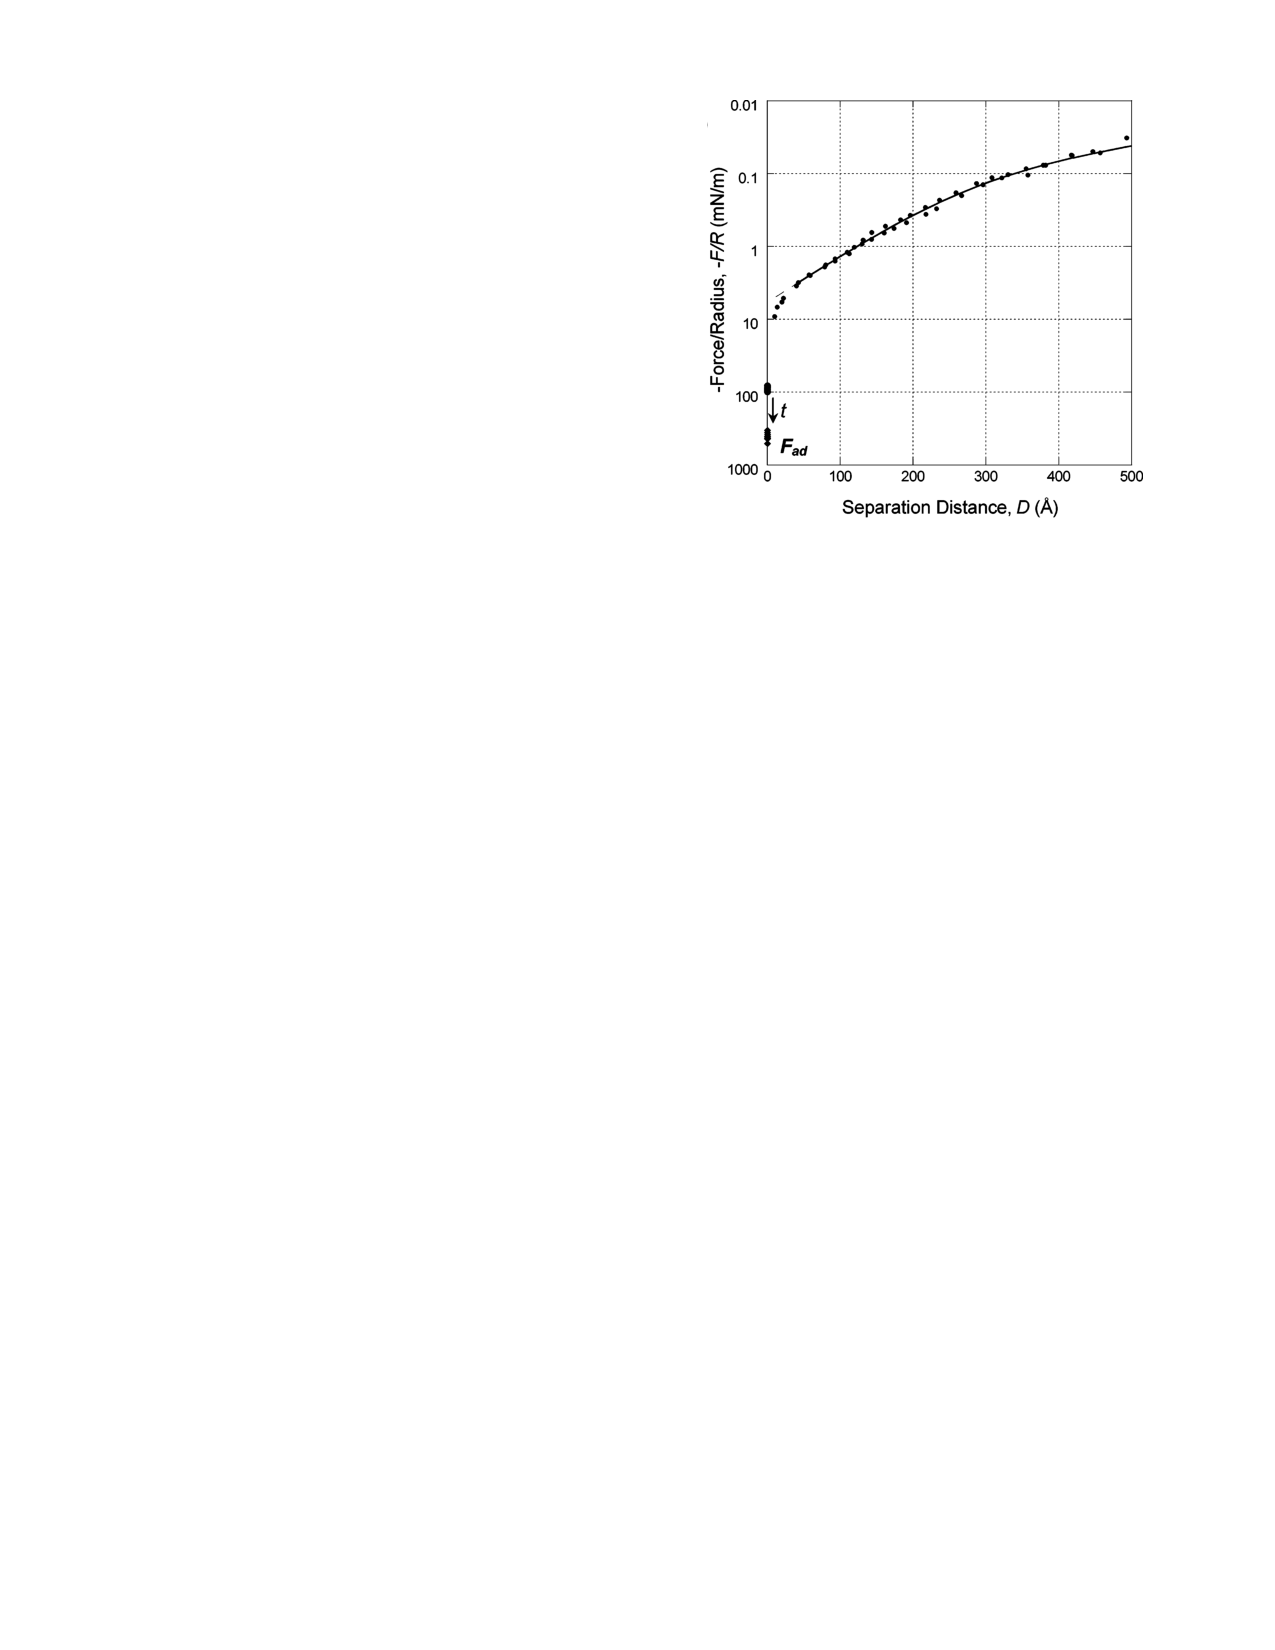
\includegraphics[width=0.35\textwidth]{figures/Background/LongRangeForce.pdf}
}
\caption{Force-distance curves for surfactant monolayers adsorbed on mica
reveal a lon-range attraction 
\cite{Lin2005}.
}
\label{fig:chandler_weeks}
\end{wrapfigure}
The hydrophobic attraction theory concerns the 
self-organization of hydrophobic particles in a viscous solvent.  
It is a phenomenological model mimicking 
the linear-response of water to surface perturbations
and was first proposed by applied mathematician 
Stjepan Mar\v{c}elja from the Australian National University in 1976.  
To explain certain repulsion measurements between lecithin bilayers,
Mar\v{c}elja and coworkers devised a mathematical
model using a Landau expansion of the free energy density 
of an order parameter for the orientation of water
\cite{LeRaPa77, MaRa76, LANDAULIFSHITZ5}.   
Their truncated free energy lead to a boundary value problem 
readily solved in terms of hyperbolic trigonometric functions
and ready 

Although simplistic, the model was general enough to 
explain a number of physical effects. 
For one, the mean orientations of water 
being opposite at the two interfaces yielded a
free energy that decreases with distance of separation
thus explaining the repulsion data for lecithin bilayers.  
Later, \cite{ClCh88,RaDe88} showed there was a 
long-range attractive force 
between hydrocarbon coated mica sheets 
following an exponential curve
and measurable up to 100 nm.  
\cite{ErLjCl89} applied the Mar\v{c}elja theory to this problem 
for an order parameter representing the excess number of
hydrogen bonds per water molecule.  

\begin{wrapfigure}[10]{r}{0.3\textwidth}
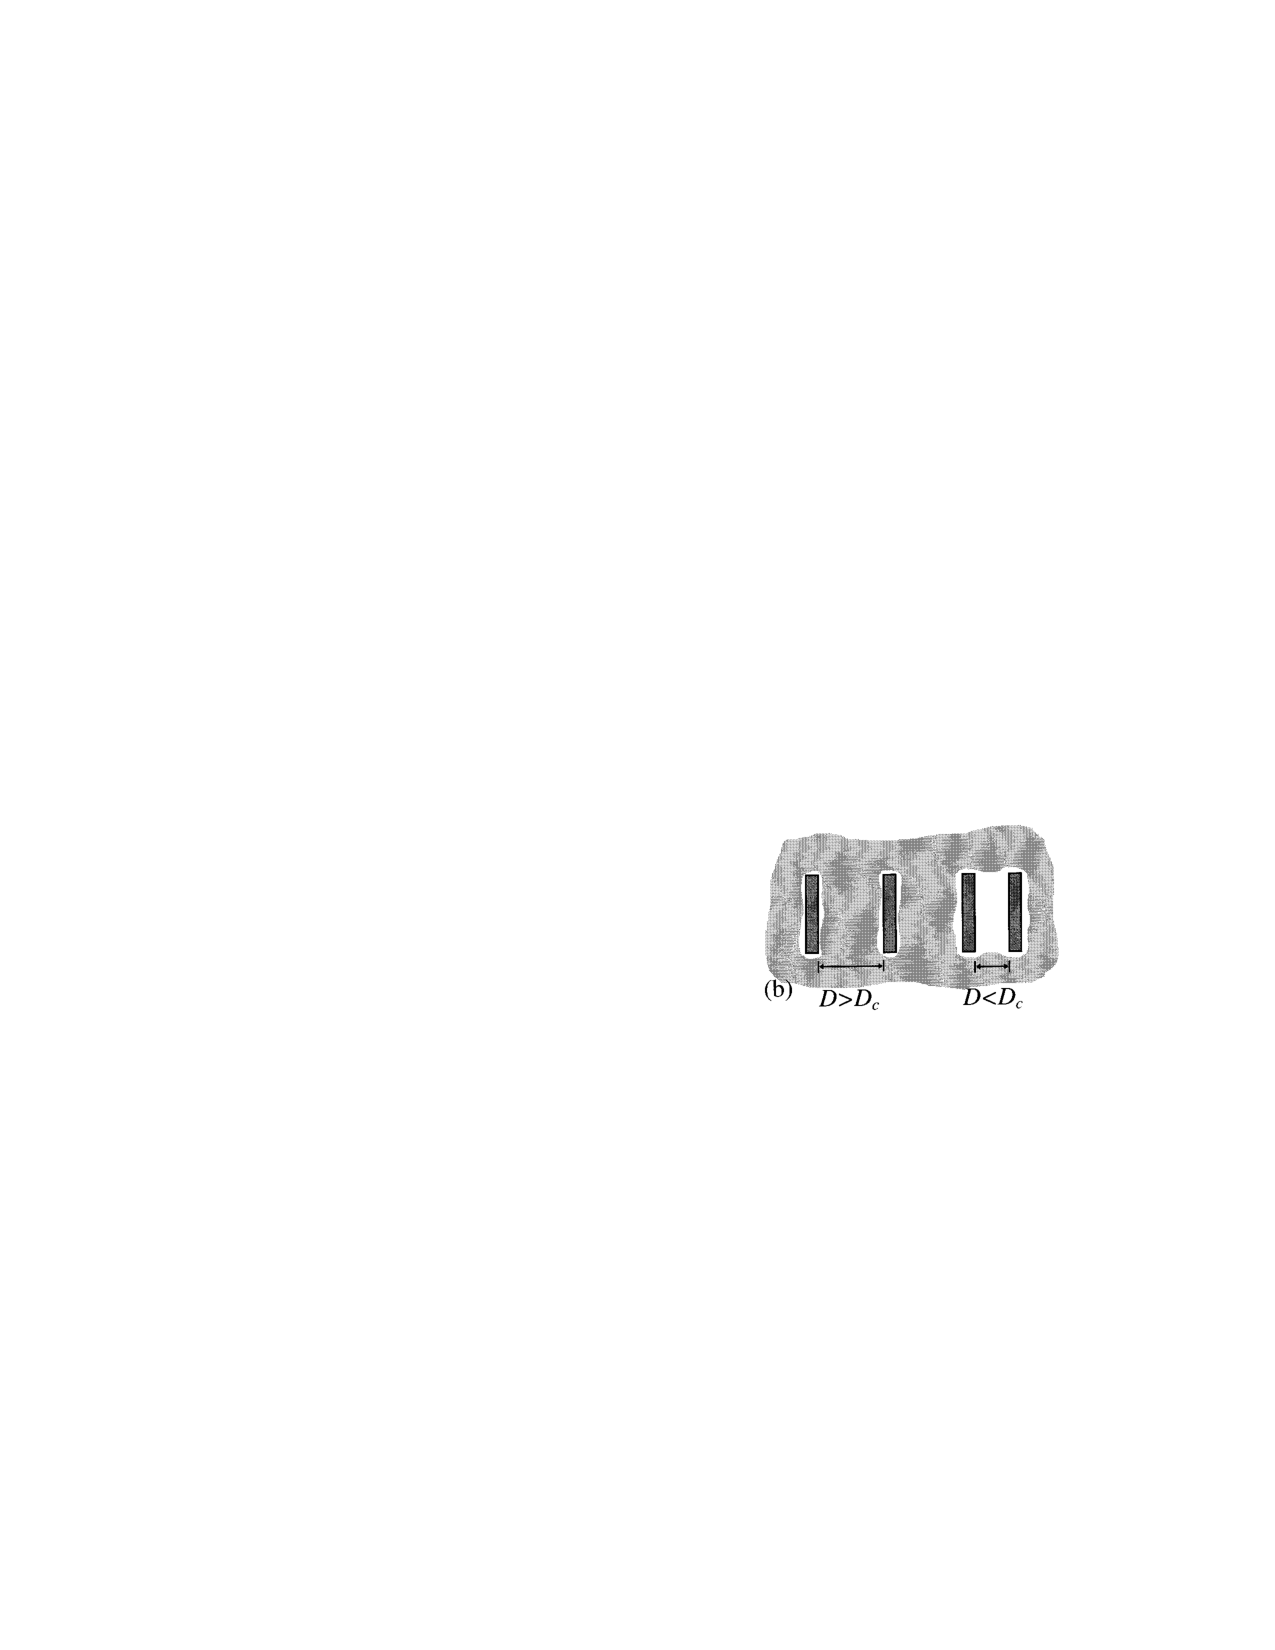
\includegraphics[width=0.3\textwidth]{figures/Background/ChandlerWeeks.pdf}
\caption{ Other theories explain hydrophobic attraction in
terms of the free energy of voids \cite{Lum1999}.
}
\label{fig:chandler_weeks}
\end{wrapfigure}
Analogues of Mar\v{c}elja's phenomenological theory 
show up in other areas related to biological self-assembly,
such as interaction of membrane-bound proteins 
\cite{KoNa15, Nagle17, KUZMIN2005}
and P. G. de Gennes's theory for the
interaction of polymer beads in mixed solvents \cite{deGe76}.
In the latter, the free energy corresponds to the
Ornstein-Zernike form of the order parameter correlation function.  
On the down side, it applies a continuum theory to
distances of a few molecular diameters, the association of
order parameter is arbitrary, it predicts monotonic forces,
and finally measured attractive forces amplify at distances below
10 nm and this feature is not accounted for by the theory
\cite{Ni80}.


\begin{wrapfigure}[22]{l}{0.3\textwidth}
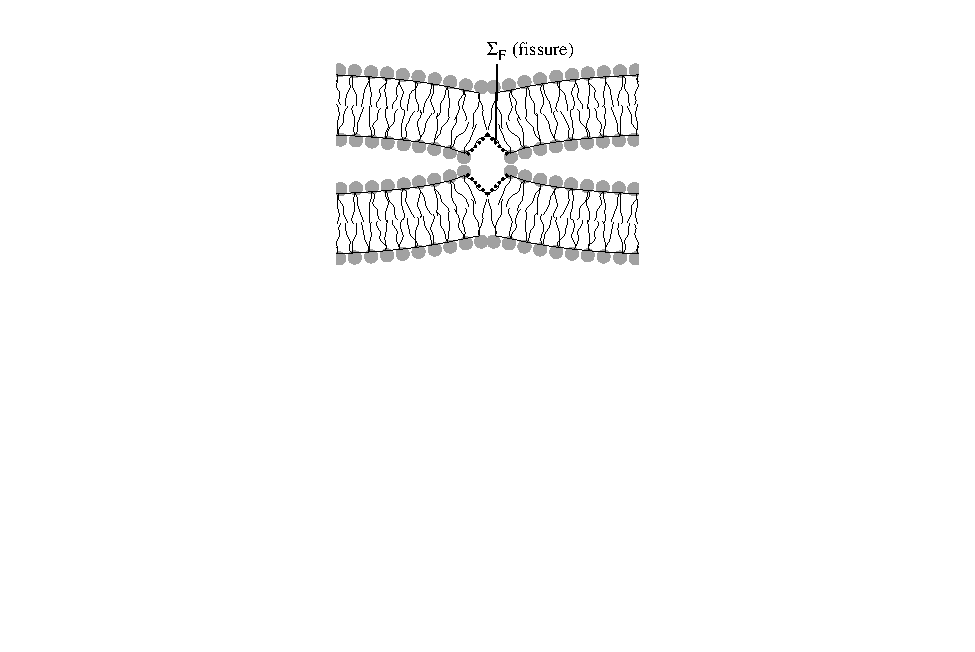
\includegraphics[width=0.3\textwidth]{figures/Background/Fissure.pdf}
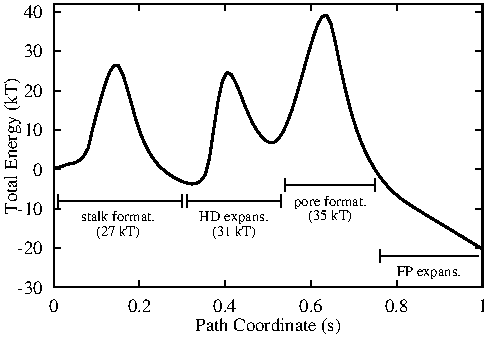
\includegraphics[width=0.3\textwidth]{figures/Background/Landscape.pdf}
\caption{
In fusion, fissures in the phospholipid monolayers expose hydrocarbon to water (top).
The energy of fissures dominates first and third stages of fusion (bottom).
}
\label{fig:fissure}
\end{wrapfigure}
Still, no single theory has beenable to account, either qualitatively or quantitatively,
for hydrophobic interaction over the full distance regime \cite{Lin2005, Meyer2006,Ducker2016}.
Despite the ubiquity of the phenomenon, theoretical developments explaining
the basic underlying principles of the hydrophobic effect have
come relatively late \cite{Ch05}. For example, studies of the partitioning of
hydrophobic solutes between water and nonpolar solvents provide
estimates for the energy cost of creating 
hydrophobic-water contacts that is a factor of three lower than
the value derived from interfacial tension measurements. Only
recently was an explanation for this discrepancy provided
\cite{Jackson2016}.

Whatever the case may be, the continuum approaches to water
structure that we present here are a conceptual advance 
that are further justified a posteriori from 
the agreement between theory and experimental surface force
curves. Researchers have used  Mar\v{c}elja's theory to calculate
energies of pore formation and fusion
\cite{Gletal88, Aketal17, RyKlYaCo16}. 
When open, the attraction between apposing hydrophobic surfaces
causes the fissure to collapse.
PI RR calculated energy barriers
of fusion using a modified form of the Helfrich
energy to include Mar\v{c}elja's free energy for the structure of 
water separating the fissures \cite{RyKlYaCo16}.
This value was later experimentally corroborated 
(Figure \ref{fig:fissure}, \cite{FrRoPi17}).

In summary, the consensus is that despite its apparent simplicity,
the predictions of the hydrophobic attraction theory are compatible
with experimental measurements and may closely reproduce the reality
of the physical process at a molecular scale \cite{FrRoPi17, Fretal21}.

In terms of applications, the approach resolves 
certain issue in soft matter modeling.
For example, the Helfrich hamiltonian from membrane biophysics
assumes a rod-like continuum but makes no use of the
amphiphilic character or lipids
\cite{Hamm2000, TerziDeserno17, PhysRevE.102.042406}.  
By coarse-graining lipids as Janus particles, we
derive the bilayer structure and elastic energies
from the amphiphilic character of constituent particles.
Moreover, the granularity of proteins and topological changes e.g.
protein induced curvature, fission, fusion, are
critical to understanding mechanical properties of membranes. 
These processes can be
modeled by standard continuum methods only with great difficulty and
excessive grid refinement.
%Assuming the location of pore nucleation,
%for example, is required in traditional continuum but is yet another
%output of our model. 
Finally, the methodology allows evolutions equations to be
computed using integral equation
methods that when optimized have near-linear in the particle number. 
%For comparison, that is the same computational cost as a finite element
%analysis of a two-dimensional membrane that ignores water.

%%%%%%%%%%%%%%%%%%%%%%%%%%%%%%
%
% The following commented out on Nov 6, 2021
%
%%%%%%%%%%%%%%%%%%%%%%%%%%%%%%%
%\section{Background}
%\label{sec:background}
%The goal of this collaborative proposal is to use mathematical modeling
%and numerical simulations to investigate the dynamic self-assembly of
%amphiphilic particles interacting via hydrophobic forces
%in solvent. Amphiphilic particles (such as lipid molecules) possess
%both hydrophobic and hydrophilic structures. In a viscous solvent they
%self-assemble into meso-/macroscopic structures (such as micelles and
%bilayers of lipids) to shield their hydrophobic parts from contact with
%the solvent (water) molecules.
%%
%%\subsection{Hydrophobic Forces}
%%\label{sec:hydrophobicforce}
%%
%Such self-assembly of amphiphiles via hydrophobic forces is ubiquitous in biology and biophysics \cite{Israelachvili1954},
%%The hydrophobic force is a ubiquitous molecular interaction in biology \cite{Israelachvili1954}, 
%and has been a major source of nonspecific interactions between
%nanoparticles in soft matter
%\cite{Sanchez-IglesiasEtAl2012_ACSNano,AltantzisEtAl2013_PSC,XieYangLuEtAl2020_COCIS}. 
%%The proposed research aims to provide fundamental understanding of the self-assembly dynamics of amphiphilic particles so to design smart materials of desirable properties by
%%tuning the geometry and properties of the amphiphilic particles. 
%
%%The hydrophobic force arises when polar solvent molecules come in contact with a non-polar substance, such as hydrocarbon or vapor.
%%In a polar solvent (like water), the dipole-dipole interaction between solvent molecules form a loosely structured hydrogen-bond network where
%%each solvent molecule shares bonds with neighboring molecules at any given time 
%%\cite{Israelachvili1954}. In the presence of  a non-polar solvent molecule loses the ability to form hydrogen bonds
%%in one direction. 
%%The decrease in the number of hydrogen bonds causes a reorientation, or structural
%%change, in the surrounding water that is energetically very unfavorable \cite{Bjorneholm2016}.
%
%
%The substantial free energy for placing hydrophobic substances in contact with water 
%is roughly proportional to the surface area of the contact region \cite{Bjorneholm2016}.  
%%As a result, hydrocarbon solutes have a large interfacial tension 
%%and try to minimize their surface area when in water. 
%At the microscopic level, the hydrophobic force is a long-range, surface
%interaction. This means that two hydrophobic surfaces, separated by
%water over some distance, experience an attractive force
%\cite{Lum1999,Meyer2006,Hammer2010}. Measurements show that the
%hydrophobic force decays exponentially with a decay length on the order of 1 nm
%\cite{Israelachvili1984, Marcelja1977,Christenson2001,Lin2005}. 
%Additionally, the interaction is not pairwise additive, meaning that
%the force between any two hydrophobic objects is altered by the presence
%of a third object, hydrophobic or otherwise \cite{SilveraBatista1242477}. 
%
%Recently, PIs RR and YNY developed a mathematical model, called the
%hydrophobic attraction potential (HAP) model \cite{Fu2018_SIAM}, that is based
%on the physical origin of hydrophobicity. This model addresses the major
%shortcomings of molecular dynamics (MD) and continuum approaches. Based
%on preliminary results (\S\ref{sec:preliminary_work}), the PIs propose to
%extend this HAP model to offer an alternative modeling methodology that
%leads to new mathematical ideas and is both physically accurate and
%computationally practical.
%%
%%
%%The word hydrophobic (water fearing) derives from the low solubility of oil (hydrocarbon solute) in water and vice versa. 
%%It causes hydrophobic moieties to aggregate and cluster,
%%is responsible for the adhesion between hydrophobic surfaces \cite{Ducker2016}, large contact angles on a 
%%dewetting surface \cite{Arenas2019,Sandre1999}, accumulation of particles along interfaces \cite{Lee2013,Lee2014}, 
%%formation of micelles and bilayers \cite{Israelachvili80}, and protein folding and membrane insertion \cite{Kabelka2018}.
%%
%%Lipids are amphiphilic molecules whose  structure possesses
%%both hydrophobic and hydrophilic parts. 
%%The amphiphilic property is what allows lipids to form the membranes and 
%%compartments of living cells \cite{Israelachvili80}. 
%%More specifically, a lipid consists of 
%%an elongated hydrocarbon tail that is hydrophobic, attached to a polar head that is hydrophilic.
%%To shield the hydrophobic tails from water, lipids self-assemble into micelles and bilayers. 
%%A micelle is a spherical arrangement of lipids with tails terminating at the micelle center. 
%%A bilayer consists of two layers of lipids called monolayers, where the lipid tails point 
%%from the monolayer surface into the bilayer core. 
%%
%%The mathematical modeling of a biological membrane is a challenging problem in applied mathematics. 
%%Bilayers are elastic and resist deformations like bending, twisting, and stretching.
%%Their elastic deformations are well described by the theory of liquid crystals \cite{ANDRIENKO2018520}.
%%Lipid bilayer membranes can also be fluidic, and the lateral translation of lipids (or any membrane bound
%%proteins) couples nonlocaly to the motion of the aqueous environment \cite{MerkelSackmannEvans1989,StoneAjdari1998_JFM,OppenheimerDiamant2009_BJ,OppenheimerDiamant2011_PRL}. 
%%%Finally, the membranes of cellular 
%%%compartments are constantly merging and pinching as part of intracellular trafficking. 
%%%Therefore monolayer surfaces undergo discontinuous deformations. 
%%
%%There are two prevailing approaches in membrane modeling, and each has its advantages
%%and disadvantages. Molecular dynamics (MD) is to date the only tool capable of resolving granular biological details
%%The computational cost of MD, however, grows with the sixth power of the sample diameter and 
%%so simulations are severely limited to 
%%small system sizes and short time scales \cite{DiCarlo2019}.
%%The other approach, continuum mechanics, assumes smooth surfaces and can therefore model 
%%realistic systems over physical times. 
%%But continuum description of a biological membrane ignores the granularity of lipid molecules, and thus requires some assumptions when a
%%membrane ruptures or when two membranes fuse \cite{ChKo08}. 
%%%
%%%mechanics presumes, rather than predicts, the nucleation of discontinuities. 
%%%
%%
%The proposed research aims to provide fundamental insight into the
%self-assembly dynamics of amphiphilic particles. These results will
%facilitate optimal design of smart materials by tuning the geometry and
%properties of the amphiphilic particles.
%
%
%\begin{wrapfigure}[9]{r}{0.24\textwidth}
%  \vspace{-20pt}
%\centerline{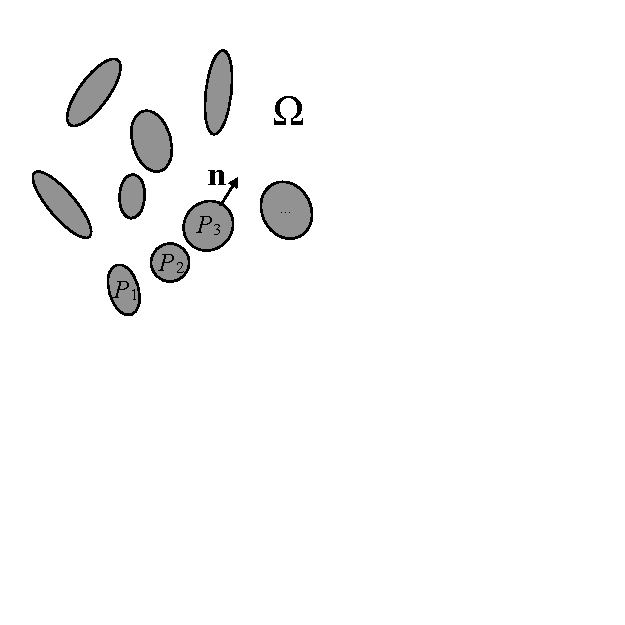
\includegraphics[width=0.23\textwidth]{figures/BG_fig1.pdf}}
%\caption{ \footnotesize
%A collection of rigid particles: $P_1,$ $P_2,$ $P_3, \ldots$. The
%exterior domain $\Omega$ represents the solvent.}
%  \label{fig:domain}
%\end{wrapfigure}
%\subsection{Hydrophobic Attraction Potential (HAP)}
%\label{sec:HAP}
%%Based on the physical origin of hydrophobicity,  we have devised a
%%functional, called the hydrophobic attraction potential (HAP), to model
%%hydrophobic forces~\cite{Fu2018_SIAM}. 
%The motivation for the HAP concept stemmed from PI RR's work concerning
%energy barriers in membrane
%fusion~\cite{RyKlYaCo16,Chetal16}. By applying a mathematical, squared-gradient
%theory for hydrophobic attraction between planar
%surfaces~\cite{Eriksson1989,Lum1999,Menshikov2017,Marcelja1977}, PI RR
%and collaborators resolved the long-standing issue of accounting for the
%energy of a monolayer fissure surface during topological transitions.
%Based on PI RR and YNY's coarse-grained membrane modeling
%work~\cite{Fu2017}, the investigators devised a gradient theory for
%arbitrary collections of hydrophobic and
%amphiphilic particles. As a new method, HAP eliminates the costly calculation
%of water by treating the solvent implicitly, is capable of representing
%biologically-relevant morphologies, and avoids complicated
%re-meshing schemes of continuum approaches by utilizing a particle-based
%representation.
%
%To define HAP, consider a collection of particles suspended in a
%solvent. The region $\Omega \subset \mathbb{R}^3$ models the solvent
%phase (Figure \ref{fig:domain}).
%%The HAP must be an energy of the shape of the region because hydrophobic
%%attraction is non-additive.
%The boundary of the region is the union of water-particle interfaces
%with unit normal $\boldsymbol{\nu}$. Some parts of this interface are
%hydrophobic while others are hydrophilic. Hydrophobic interfaces disturb
%the hydrogen bond structure of water~\cite{Luzar1987, Jonsson2006,
%Varilly2011} and this disturbance comes with an energetic penalty that
%is proportional to interfacial area. There is an additional decay
%length, due to rapid fluctuation in the hydrogen bond network,
%describing how far the restructuring extends into bulk water.
%
%The above considerations motivate the following definition for HAP:
%\begin{align}
%\label{HAP}
%  \Phi = \gamma \int_{\Omega} \rho |\nabla u|^2 + \rho^{-1}u^2 \,\dif V. 
%\end{align}
%The integrand contains
%the decay length $\rho$
%and a dimensionless scalar function $u(\mathbf{x})$ called the water activity.
%The integrand has units of an inverse length, so
%the volume integral has units of area. Multiplication by interfacial tension
%$\gamma$ makes $\Phi$ an energy. 
%
%To establish an attraction between interfaces, the water activity is not
%arbitrary but rather is the solution of the screened Laplace
%equation boundary value problem 
%\begin{equation}
%  \label{SL}
%  -\rho^2 \Delta u + u = 0, \mbox{ } \mathbf{x} \in \Omega, \qquad
%  u = f,  \mbox{ } \mathbf{x} \in \partial \Omega, \qquad 
%  u(\mathbf{x}) \to 0, \mbox{ as } |\mathbf{x}| \to \infty.
%\end{equation}
%The boundary values $f$ define the degree of hydrophobicity of the
%water-particle interface: $f=1$ describes a hydrophobic interface, and
%$f=0$ describes a hydrophilic interface. Thus, $f$ encodes information
%about the particles, and the parameters $\rho$ and $\gamma$ encode
%information about the quality of the solvent~\cite{Israelachvili1954,
%Discher2002}.
%In the figures throughout the proposal, red is for $u = 1$ and blue is for $u = 0$.
%In practice, we integrate~\eqref{HAP} by parts and
%use~\eqref{SL} to obtain
%\begin{equation}
%\label{eq:HAP_easy}
%\Phi = -\gamma \int_{\partial \Omega} \rho u \nabla u \cdot \boldsymbol{\nu} \,\dif S,
%\end{equation}
%thereby avoiding volume integral calculations.
%
%The equations~\eqref{HAP} and~\eqref{SL} possess a number of
%mathematical properties that mirror the phenomenological characteristics
%of hydrophobic attraction. Specifically, solutions of~\eqref{SL} yield
%an attractive force between hydrophobic bodies separated by water, and
%this attraction decreases exponentially with the distance of
%separation~\cite{Eriksson1989}. Using boundary layer analysis, the HAP
%converges to a surface energy in the zero-decay length
%limit~\cite{Lee2018, Lin2015, Shibata2004}. Finally, we have
%demonstrated that the forces derived from HAP theory are
%non-additive~\cite{Meyer2006, Fu2018_SIAM}. 
%%The hydrophobic force has been implicated in the directed folding of proteins, 
%%adhesion between biological membranes, but it is still unanswered as to whether
%%the hydrophobic force of the form (\ref{HAP}--\ref{SL}) exists between small molecules. 
%
%%As a summary of its mathematical properties,  the hydrophobic force
%%is a non-additive, exponentially decaying surface force 
%%that possesses a separation of length scales. These properties suggest 
%%a boundary value problem formulation of the hydrophobic force.  
%%The non-additivity of the hydrophobic force has to do with the fact that there is no superposition
%%principle for including subdomains in boundary value problems. 
%%The exponential decay is a property of a second order elliptic partial differential equation (PDE). 
%%Finally, the separation of scales come from boundary layers, 
%%where the energy of the boundary layer in the zero-thickness limit corresponds to macroscopic interfacial tension.
%%Overlapping boundary layers correspond to microscopic hydrophobic attraction, 
%%and the boundary layer thickness corresponds to the decay length of attraction.
%%
%%
%%\section{Previous Results by the PIs}
%%\label{sec:results}
%%
%%%In our paper \cite{Fu2018_SIAM}, 
%%PIs RR and YNY developed the HAP model (\ref{HAP}--\ref{SL})
%%to quantify the macroscopic assembly and mechanics of a lipid bilayer membrane in solvents \cite{Fu2018_SIAM}.
%%%We formulated the boundary value problem as a second-kind
%%%integral equation (SKIE), presented in the Section (). 
%%%The simulated fluid-particle systems exhibit a variety of multiscale behaviors over both time and length.
%%%Over short time scales, the numerical results showed self-assembly for model lipid particles. 
%%%For large system simulations, the particles formed realistic configurations like micelles and bilayers. 
%%%Our collections showed that these amphiphilic particle bilayers  possessed mechanical properties of a 
%%%lipid  bilayer  membrane  that  are  consistent  with other results in the literature.   
%To define the particle dynamics, let $P_1$, $P_2$, \ldots, $P_N$ be a
%finite collection of disjoint, rigid, and closed particles each with
%a Lipschitz boundary. Assume that the label $f$ is an element of the
%Sobolev space $H^1(\Omega)$. The functional~\eqref{HAP} has a minimizer
%among all functions $u$ equaling $f$ on the boundary in the sense of
%trace. Conversely, from maximum principles and energy estimates, the
%solution of~\eqref{SL} is unique and minimizes~\eqref{HAP}. Taking the
%first variation of~\eqref{HAP}, i.e.~the derivative with respect to the
%domain~\cite{Bandle2015, Schiffer1954, Grinfeld2010}, yields a
%symmetric, rank-two tensor called the hydrophobic stress (equation (2.3)
%in~\cite{Fu2018_SIAM}):
%\begin{align}
%  \label{stress}
%\boldsymbol{\sigma}_{\text{hydro}} = \gamma \rho^{-1} u^2 I + 2\rho
%  \gamma \left(\frac{1}{2}|\nabla u|^2I - \nabla u \nabla u^T\right).
%\end{align}
%%
%%To obtain \eqref{stress}, we observe that the potential $\Phi$ is a function of the particle position and orientations.
%%This is because the particle configuration defines the shape of $\Omega$ and the boundary data $f.$ 
%%Taking the derivative of \eqref{HAP} with respect to particle configurations, and using the boundary value problem \eqref{SL}
%%in a critical way leads to the surface term \eqref{stress}.  
%%
%Integrating the hydrophobic stress over the surface of particle $P_i$
%reveals the hydrophobic force, and torque on each particle 
%\begin{align}
%  \label{forceandtorque}
%  \mathbf{F}_{\text{hydro},i} = \int_{\partial P_i} \boldsymbol{\sigma}_{\text{hydro}}
%  \cdot \boldsymbol{\nu} \,\dif S,\quad
%  \mathbf{G}_{\text{hydro},i} = \int_{\partial P_i} (\mathbf{x}-\mathbf{a}_i) \times
%  (\boldsymbol{\sigma}_{\text{hydro}} \cdot \boldsymbol{\nu}) \,\dif S,
%\end{align}
%relative to the center of mass $\mathbf{a}_i$. This system is force- and
%torque-free (\S\ref{subsec:specific_aim_2}). To avoid particle
%collisions, we define an excluded volume potential $\Phi_{\text{repul}}$
%that diverges whenever tubular neighborhoods of adjacent particles
%overlap. The total potential, force, and torque are then
%\begin{equation}
%\label{eq:total_poten}
%\Phi = \Phi_{\text{hydro}} + \Phi_{\text{repul}},\quad
%\mathbf{F}_{i} = \mathbf{F}_{\text{hydro},i} + \mathbf{F}_{\text{repul},i},\quad
%\mathbf{G}_{i} = \mathbf{G}_{\text{hydro},i} + \mathbf{G}_{\text{repul},i}.
%\end{equation}
%
%To supply viscous dissipation, we incorporate the mobility problem
%flow for a rigid body suspension in Stokes flow:
%\begin{equation}
%\label{eq:stokes}
%\begin{aligned}
%  &-\mu \Delta \mathbf{u} + \nabla p = 0, \quad \mathbf{x} \in \Omega, \qquad 
%  \nabla \cdot \mathbf{u} = 0,  \quad \mathbf{x} \in \Omega,\\
%  &{\bf u}(\mathbf{x}) \to 0 \quad \text{as}\ |\mathbf{x}|\to \infty,\qquad 
%  \mathbf{u}(\mathbf{x})|_{\partial P_i} = \mathbf{v}_i +
%\boldsymbol{\omega}_i\times(\mathbf{x} - \mathbf{a}_i),\\
%&\int_{\partial P_i}\boldsymbol{\sigma}\cdot {\bf n} \dif S=-{\bf F}_i, \quad
%\int_{\partial P_i} (\mathbf{x} - \mathbf{a}_i)\times (\boldsymbol{\sigma} \cdot \mathbf{n}) \dif S =-{\bf G}_i.
%\end{aligned}
%\end{equation}
%Here, $\mu$ is the fluid viscosity; the first two equations state that
%the fluid motion is a divergence-free Stokes flow; the third equation
%specifies that the fluid velocity vanishes at infinity; the fourth
%equation enforces a rigid body motion on each particle, where
%$\mathbf{v}_i$ and $\boldsymbol{\omega}_i$ are unknown translation and
%angular velocities; and the last two equations state that the net
%viscous forces and torques with fluid shear stress $\boldsymbol{\sigma}$
%balance \eqref{eq:total_poten}.
%
%
%The time integration of particle configurations goes as follows:
%\textbf{(i)} solve the BVP~\eqref{SL} for the screened Laplace equation,
%\textbf{(ii)} determine the rigid body forces and
%torques~\eqref{forceandtorque}, \textbf{(iii)} solve the Stokes mobility
%problem~\eqref{eq:stokes} for the rigid body motions, and \textbf{(iv)}
%update the particle configuration.  Numerical challenges and how these
%challenges are overcome are described in \S\ref{subsec:specific_aim_2}.
%
%%%(2YY: 
%%We have intentionally ignored  latency in the variational 
%%calculations. At issue is that any change in the particle position involves the relaxation time 
%%of the hydrogen bond network. To remedy this, we could parametrize a path for the 
%%particles configuration as a function of physical time. Then the rate of change
%%of hydrophobic interaction includes the surface hydrophobic stress as calculated, but also a body term 
%%for time change of activity, assuming we model hydrogen bond relaxation by diffusion. 
%%The diffusion time, however, is extremely small since hydrogen bond lifetimes are on the order 
%%of $10^{-11}$ s \cite{Israelachvili1954}. This setup is analogous  to that of a Kelvin-Voigt material,
%%where viscoelastic deformations exponentially approach the purely elastic deformation.  
%%%)
%
%\begin{wrapfigure}[14]{l}{0.35\textwidth}
%\centerline{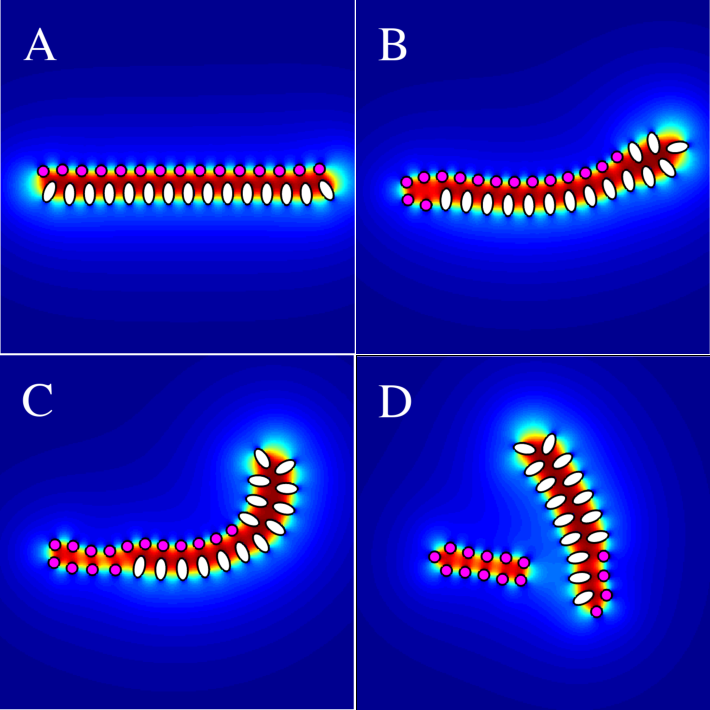
\includegraphics[width=0.34\textwidth]{figures/PW_fig2.pdf}}
%  \vspace{-8pt}
%  \caption{\label{fig:demixing} \footnotesize An initial assembly of
%  small and large particles spontaneously segregates into two smaller
%  bodies.}
%\end{wrapfigure}
%The HAP formulation is, to our knowledge, the first demonstration of
%bilayer self-assembly by a continuum-based interaction
%model~\cite{Noguchi2001, Farago2003, Brannigan2006, Brooks2009,
%Wang2013}. Our simulations use Janus particles to model lipid
%amphiphiles which are popular in material science and physics for
%creating functional materials~\cite{Lee2014, Lee2013}. Janus particles
%are typically spherical with a biphasic material label on either
%hemisphere, endowing the particle with
%a directional order. We model an
%elongated lipid by elliptical particles with the hydrophobic label
%defined along the ellipse's axis. 
%Under the hydrophobic force, with
%excluded volume, the Janus particles spontaneously merge and realign
%to form bilayers. This occurs only as a result of energy minimization
%and does not require artificial inputs.
%%
%
%%
%It is worth emphasizing that the HAP model uses only a few parameters:
%interfacial tension, decay length, repulsion strength, and particle
%shape. For example, an elastic modulus for stretching a vesicle from
%micropipette manipulation calibrates our interfacial tension
%parameter. This is in direct contrast with pair-potential-based
%approaches in MD simulations and coarse-grained models where many more
%parameters are required~\cite{Varilly2011, Wang2013}.
%%MD simulators have also made measurements and lately there is better and better agreement with reality. 
%%But even the simplest coarse grained models based on pair potentials for lipids has many more parameters \cite{Varilly2011,Wang2013} . 
%
%%As a proof of concept, our work has already tested for elastic energies
%%for bending, stretching, and tilt of the bilayer assembly. The elastic
%%coefficients derived from the HAP simulations show strikingly positive
%%agreement with experimentally determined values~\cite{Fu2018_SIAM}.
%%Encouraged by these results and the hydrodynamic simulations of
%%bilayer assembly, the PIs propose to extend the HAP model to make direct
%%comparisons with experimental results \S\ref{subsec:specific_aim_1} and to
%%establish that the HAP model has the capability to model
%%flow phenomena across length scales and time scales
%%\S\ref{subsec:specific_aim_2} using efficient, high-order numerical
%%methods \S\ref{subsec:specific_aim_3}.
%
%%\begin{wrapfigure}[14]{l}{0.35\textwidth}
%%\centerline{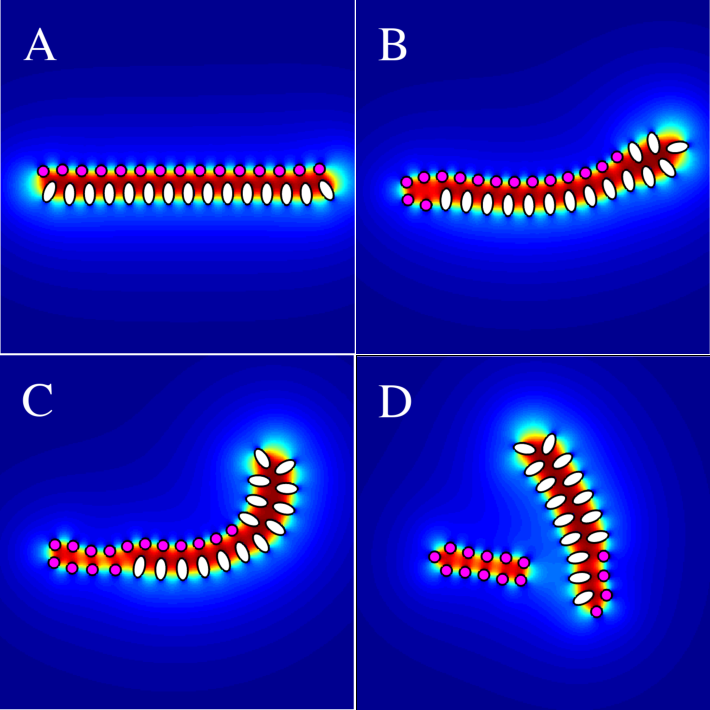
\includegraphics[width=0.35\textwidth]{figures/PW_fig2.pdf}}
%%  \vspace{-8pt}
%%  \caption{\label{fig:demixing} \footnotesize An initial assembly of
%%  small and large particles spontaneously segregates into two smaller
%%  bodies.}
%%\end{wrapfigure}
%Over the past decades, researchers have used a number of mathematical
%tools to simulate vesicles in a shear flow, including lattice
%Boltzmann~\cite{KaouiHartingMisbah2011_PRE}, coarse-grained Brownian
%dynamics~\cite{NoguchiTakasu2002_BJ}, phase
%field~\cite{DuLiuWang2004_JCP,BibenKassnerMisbah2005_PRE}, level
%set~\cite{DoyeuxGuyotChabannesEtAl2013_JCAM}, boundary
%integral~\cite{Shravan09,Rahimian15}, and immersed boundary
%approaches~\cite{KimLai2010_JCP,KimLai2012_PRE,HuLaiSeolEtAl2016_JCP}.
%Most of these approaches assume a mathematical surface, whether
%implicitly or explicitly, and define an elastic bending energy of the
%surface. These vesicle studies built off of numerical methods for
%calculating energy minimizing steady equilibrium shapes of lipid bilayer
%membranes, vesicles, and red blood cells. These approaches range from
%the finite element~\cite{Bartels,Peng13,RyKlYaCo16,Sinha15},
%phase field~\cite{Du05,QiangDu08,Lowengrub13}, and immersed
%boundary methods~\cite{Hu,Hu13, KimLai2010_JCP}. PI RR and collaborators
%led in part the development of phase field functionals of membrane
%elastic energy and approaches to coupling membrane elasticity to
%fluids~\cite{0951-7715-18-3-016,Du05,DuEuler,QiangDu09}.
%
%
%%The vesicle obeys fluid
%%transport and in turn the fluid balances shear stress with the vesicle's bending force. 
%
%Our HAP approach differs from these prior methods in a number of
%respects. First, we do not assume a surface. Rather, we 
%assume a collection of amphiphilic particles. The
%collection of amphiphiles minimize hydrophobic interactions by
%sequestering hydrophobic tails in the form of a bilayer, and the
%particles' excess free energy gives rise to an elastic bilayer energy.
%The second difference lies in the fluid-interface coupling. Here, the
%associated mobility problem~\eqref{eq:stokes} is more complicated than
%dealing with a stress boundary condition or diffusive surface force
%because the fluid velocities are for individual rigid body motions at each
%particle surfaces. Finally, the HAP model directly addresses the
%existence of multiple phases. We can vary lipid length, spontaneous
%curvature, and bending rigidity by introducing different particle shapes
%and hydrophobic boundary conditions (Figure~\ref{fig:demixing}). In
%contrast, continuum theory deals with multiple phases through additional
%surface densities that must satisfy specialized transport
%equations~\cite{Lowengrub07, MikuckiZhou17}. 
%
%
%\begin{wrapfigure}[6]{r}{0.35\textwidth}
%\centerline{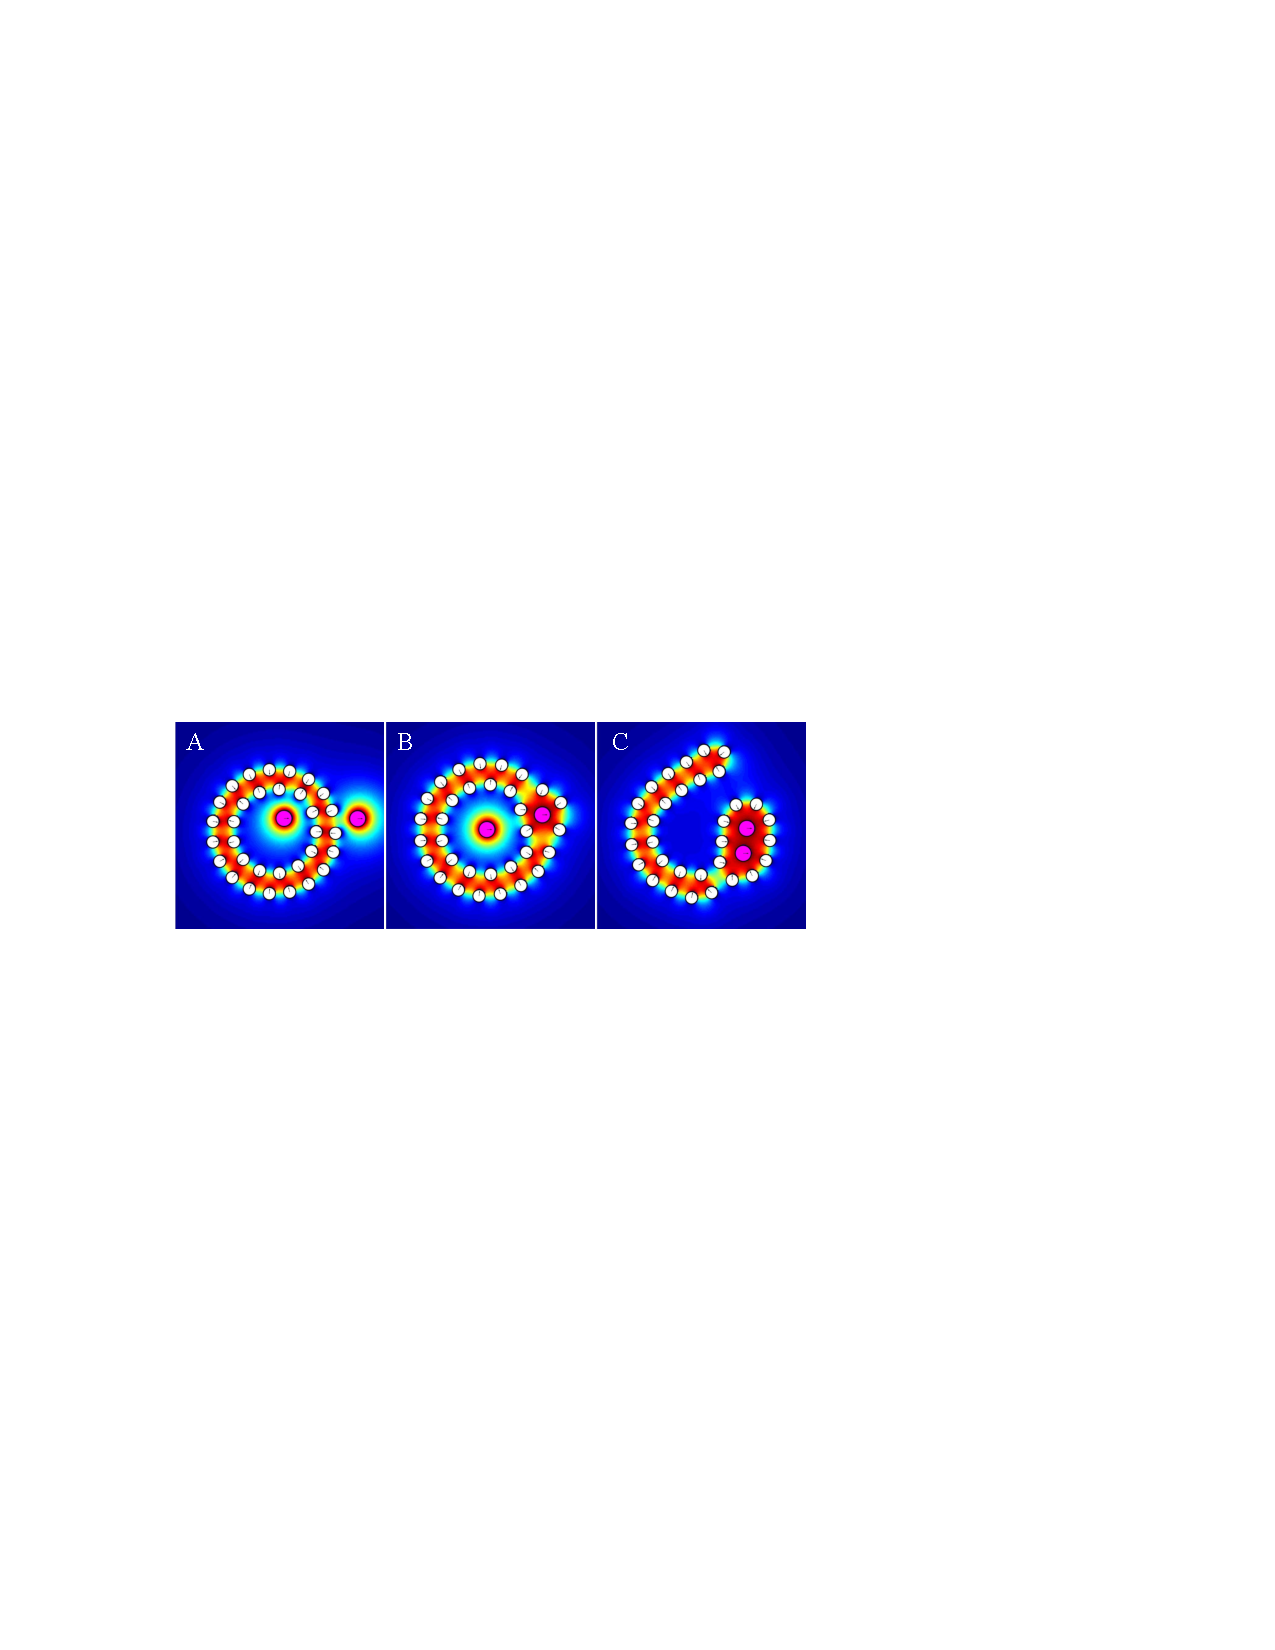
\includegraphics[width=0.34\textwidth]{figures/Lysis.pdf}}
%  \vspace{-8pt}
%  \caption{\label{fig:lysis} \footnotesize Two hydrophobic particles
%  enter and then lyse the circular bilayer.}
%\end{wrapfigure}
%The greatest strength of using the HAP to model a lipid bilayer membrane is
%the ability to form discontinuities (interfacial singularities) from first
%physical principles without any artificial manipulation to rearrange the
%interface (Figures~\ref{fig:demixing} and~\ref{fig:lysis}). For
%example, using the HAP model to simulate a vesicle under a shear flow
%that is strong enough to cause the vesicle membrane to rupture (see
%\S\ref{sec:preliminary_work}), we expect the HAP model to capture the
%reorganization of lipid molecules on the scales of membrane thickness
%($\sim 5$ nm), which is a nearly impossible task using phase-field or
%immersed boundary methods without extreme refinement around the membrane
%and artificial treatment of reconnection during the topological change
%of an interface \cite{doi:10.1063/5.0009734, LiAn-Chang16,
%doi:10.1098/rspa.2012.0505, doi:10.1137/130941432, Feetzl18,
%doi:10.1137/16M1108406}.
%
%%Some disadvantages are that the hydrophobic interaction does not constrain vesicle volume. 
%%Instead, changes in volume are rate limited by inter-particle spacing,
%%which may be undesirable in case of a mathematically strict volume constraint.
%%% set vesicle volume, as is done in the study of liposomes
%%%using auxiliary constraint equations for instance. 
%%%Also, the boundary integral method formulation
%%%relies on linearity of the Stokes equations. There has been some progress in
%%%boundary integral methods for the non-linear Navier-Stokes equations [ref].
%%%We point out that some non-Newtonian effects in polymers are a consequence of hydrophobic
%%%and steric molecular interactions like the ones presented in this proposal. 
%
%
%
%
%
%%
%%
%%The next few years provide the ideal window of opportunity for demonstrating the physical realism 
%%of the HAP model. 
%%
%%
%%
%%The definitions and calculations for fully three-dimensional bilayer elastic energies are described in greater
%%detail in Specific Aim 1. 
%%
%
%
%% 4.1 pN / nm = 4.1 pN nm / nm^2 = 4.1(1e-12)(1e-9) N m/(1e-18) m^2 = 4.1 (1e-3) J/m^2 = 4 mJ/m^2 
%% pN/nm = mJ / m^2 and 1 kT / nm = 4 mJ / m^2 so stretching 40 gives 40  
%% erg / cm^2 =  (1e-7) J/(1e-4) m^2 =   1e-3 J/m^2 =  mJ/m^2  
%% 120 mJ / m^2 
%% 10 erg / cm^2 = 10 pN nm / nm^2 = 2 kT / nm^2 
%%
%
%%\section{Proposed Research}
%%\label{sec:proposed-work}
%%The goal of the proposed research is to develop fast,
%%high-order-accurate, parallel numerical algorithms for large-scale
%%simulations of the collective hydrodynamics of janus particles in a solvent in both two- and three-dimensions.
%%First we summarize some basic formulation and preliminary results
%%\cite{Fu2018_SIAM} in \S~\ref{subsec:bie} and \S~\ref{subsec:3dbie}.
%%We then describe outstanding numerical issues that we propose to address  in \S~\ref{subsec:proposed_research}.
%
%%\section{Proposed Research}
%%\label{sec:proposed-work}
%%The goal of the proposed research is to develop fast,
%%high-order-accurate, parallel numerical algorithms for large-scale
%%simulations of the collective hydrodynamics of  amphiphilic particles in a viscous solvent.
%%%
%%Based on the integral formulation in \S~\ref{subsec:bie} and \S~\ref{subsec:3dbie}, we have demonstrated that 
%%our potential theory approach can efficiently simulate self-assembly of 
%%amphiphilic particles into two-dimensional micelles, bilayer membranes,
%%and vesicles \cite{Fu2018_SIAM}.
%%%
%%While these results show great potentials in simulating the collective hydrodynamics of amphiphilic particles and
%%reproducing mechanical properties of their bilayer assembly, 
%%several outstanding issues need to be addressed for such approach to be efficiently applied to three-dimensional 
%%collective hydrodynamics of amphiphilic particles.
%%
%%the two-dimensional hydrodynamics of amphiphilic particles 
%%
%%the two-dimensional results in \cite{Fu2018_SIAM} are in agreement with the 
%%
%%
%%First we summarize some basic formulation and preliminary results
%%\cite{Fu2018_SIAM} in \S~\ref{subsec:bie} and \S~\ref{subsec:3dbie}.
%%We then describe outstanding numerical issues that we propose to address  in \S~\ref{subsec:proposed_research}.
%% -----------------------------------------------------------------------------
%%\subsection{Proposed research: High-order discretization of surface integrals in three dimensions}\label{subsec:proposed_research}
%%% -----------------------------------------------------------------------------
%%% {{{
%%The practical application of integral equation methods requires the
%%accurate evaluation of boundary integrals with singular, weakly
%%singular or nearly singular kernels.  Historically, these issues have
%%been handled either by low-order product integration rules (computed
%%semi-analytically), by local modifications of a smooth
%%rule~(e.g.~\cite{alpert,kapur,sidi}), by singularity
%%subtraction/cancellation (e.g.~\cite{duffy,bruno1,bruno2,davis_1984,graglia_2008,hackbusch_sauter_1994, jarvenpaa_2003,khayat_2005,kress_boundary_1991,schwab_1992, ying_2006}), by kernel
%%regularization and asymptotic analysis (e.g.~\cite{beale1,beale2,goodman_1990, haroldson_1998, lowengrub_1993,schwab_1992}), or by the
%%construction of special purpose ``generalized Gaussian'' quadrature
%%rules (e.g.~\cite{ggq1,ggq2,ggq3}).
%%In the complex analytic case, additional methods
%%have been developed by \citet{helsing_2008a} for off-surface
%%evaluation. It should be noted that in the two-dimensional case,
%%several of these alternatives provide extremely effective schemes,
%%especially the kernel-splitting method developed by Johan Helsing
%%\cite{helsing_integral_2009,helsing_tutorial_2012,helsing_2008a} since
%%they all permit local adaptivity and high order accuracy.
%%
%%The high-order quadrature rules for the evaluation of surface integrals
%%in three dimensions are much less developed than the line integrals in two
%%dimensions. For example, there are no Gaussian quadratures for integraing
%%polynomials on a flat triangle, even though efficient quadratures
%%\cite{xiao2010cma,vioreanu2014} have been
%%developed recently for such purpose. For weakly singular or singular integrals,
%%\cite{bremer2012jcp,bremer2013jcp} constructed high-order quadratures
%%for surface integrals on a general triangle, while \cite{gimbutas2013sisc}
%%presented a fast algorithm for integrating $1/r$-type singular integrals
%%for surfaces that are homeomorphic to a sphere. We would like to propose
%%to study the so-called quadrature by expansion (QBX) scheme~\cite{klockner2013jcp,qbx2}
%%for the evaluation
%%of both singular and near-singular surface integrals encountered in the
%%discretization of BIEs in three dimensions. Conceptually, the idea of the QBX
%%to evaluate singular, hypersingular and near singular integrals
%%on smooth surfaces is more or less straightforward. That is, the surface is discretized
%%into smooth triangles and smooth high-order quadratures are applied to evaluate
%%the expansion coefficients
%%on all source triangles with the QBX expansion center placed at a point off the surface.
%%One may then form a suitable expansion (for example, a Taylor expansion) around that
%%center and evaluate this expansion back at the target point on the surface (or close
%%to the surface in the near singular case). Compared to the competing aforementioned
%%quadrature schemes, the QBX quadrature is attractive
%%because it offers a clear path for being extended to: \textbf{(1)}
%%handle any ambient and source dimensionality, \textbf{(2)} integrate
%%any kernel, and thereby be usable for a very large range of PDEs and
%%boundary conditions, \textbf{(3)} handle any singularity, including
%%hypersingular operators, \textbf{(4)} be usable with any high-order surface
%%discretization, \textbf{(5)} generate well-conditioned discrete
%%operators to which iterative methods such as GMRES~\cite{gmres} can be
%%applied in a black-box fashion, \textbf{(6)} be computationally
%%efficient enough to be applied on the fly (without the need to store
%%quadrature tables), \textbf{(7)} integrate well with fast algorithms
%%such as the Fast Multipole Method. 
%%
%%In practice, there are still many issues that need to be resolved.
%%For example, there are now many variants of QBX including global and local
%%QBX~\cite{klockner2013jcp,rachh2017jcp}, the target-specific QBX~\cite{siegel2018jcp},
%%kernel-independent QBX~\cite{abtin2018bit}, and
%%quadrature by two expansions~\cite{ding2019arxiv}. The coupling of the QBX
%%and the FMM may also lead to certain instability issues which may require
%%some changes in the fast multipole method~\cite{wala2018jcp}. Similar
%%to other quadrature methods, there have been an extensive study on the QBX
%%methods in two dimensions, while its three dimension
%%version~\cite{wala2019jcp,af2018sisc,siegel2018jcp,wala2019arxiv} has not been
%%fully studied and the implementation is even more scarce. We plan to investigate
%%the accuracy and the convergence order of the various QBX schemes mentioned above,
%%its coupling with the FMM, parallel implementation issues for large-scale
%%problems, and the application to our target problems.




\begin{figure}[!]
\begin{center}
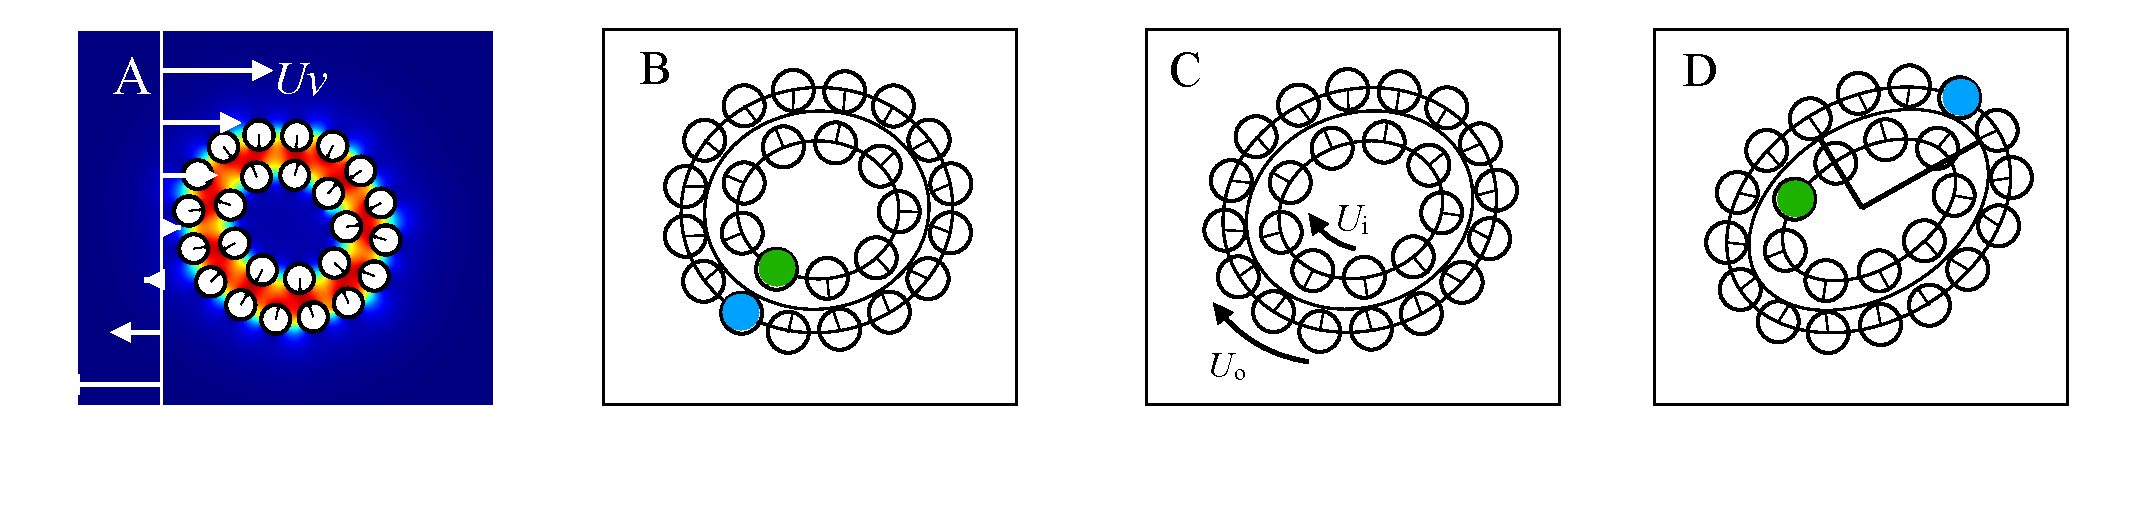
\includegraphics[width=1\textwidth]{figures/PW_fig1A-D.pdf}
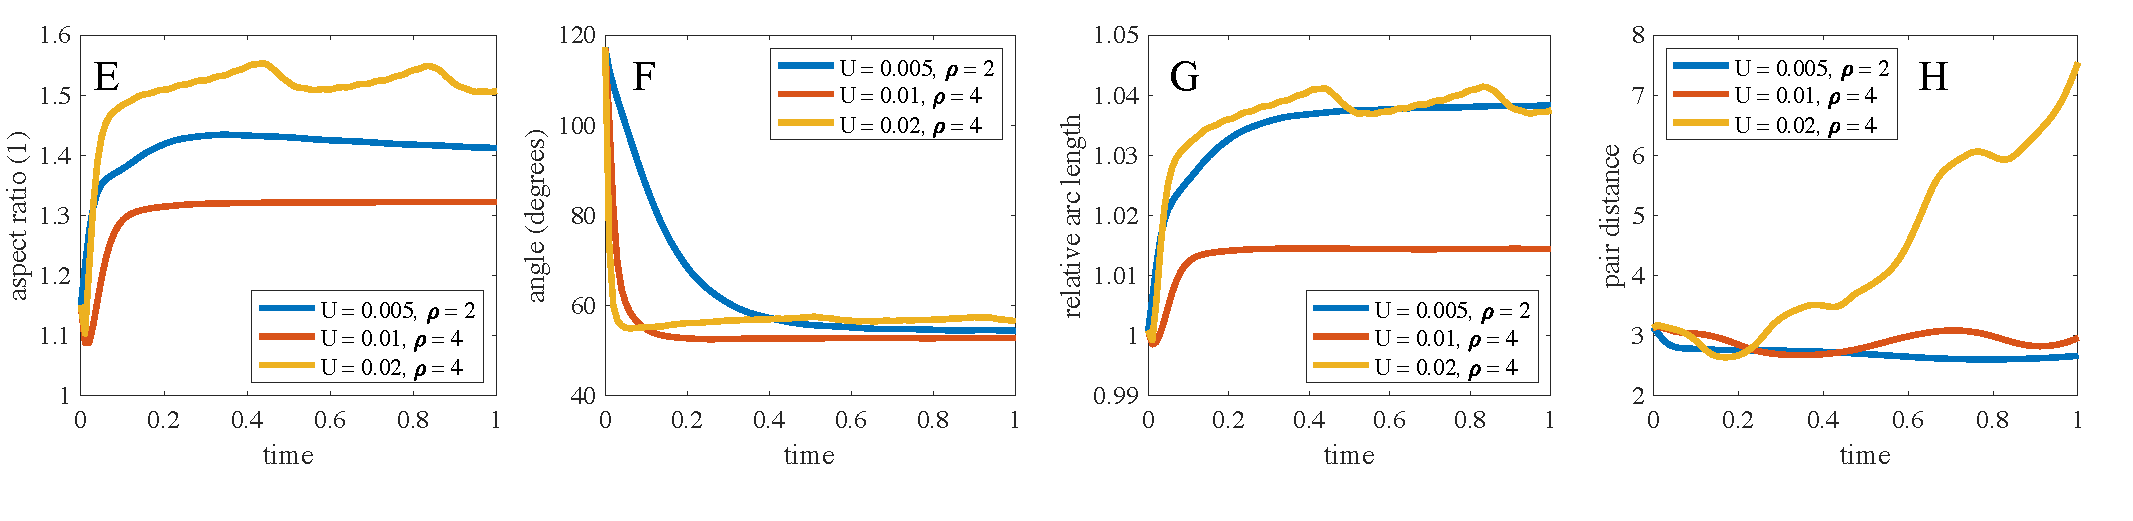
\includegraphics[width=1\textwidth]{figures/PW_fig1E-H.pdf}
\end{center}\vspace{-0.3in}
\caption{(A) A vesicle formed by amphiphilic particles in shear flow,
  and the tank-treading motion (B)--(D). The separation of particle
  pairs in (B) and (C) illustrate inter-leaflet slip.  (E)--(G)
  Tank-treading reaches a steady state in elliptical aspect ratio,
  major-axis angle, and circumference.}
\label{fig:tanktreading}
\end{figure}
\section{Preliminary Work on Two-dimensional Vesicle Hydrodynamics in Shear Flow\label{sec:preliminary_work}} 
%The motion of vesicles in shear flow is an important
%problem in the applied mathematics because simulations can reveal mechanical
%properties of membranes and lead to an enhanced understanding of 
%deformable particle laden flows \cite{Sinha15}. 
%
To implement a vesicle in shear flow in the context of hydrophobic potentials and mobility problem, 
we consider a shear flow in the far-field $\mathbf{u}_{\infty} = Uy\mathbf{i}_x$ in the direction of the $x$-axis
(Figure \ref{fig:tanktreading}A).
%
%This field satisfies the linear Stokes system but does not give rise to a rigid motion at the particle interfaces. 
%To have a rigid motion, we change variables $\mathbf{u} = \tilde{\mathbf{u}}+ \mathbf{u}_{\infty}$ and 
%for the new field $\tilde{\mathbf{u}}$ vanishing at infinity we let 
%$\tilde{\mathbf{u}}|_{\partial P_i} = \mathbf{v}_i + \boldsymbol{\omega}_i \times (\mathbf{x} - \mathbf{a}_i)$ 
%where $(\mathbf{v}_i,\boldsymbol{\omega}_i)$ are the unknown translation and angular velocities of the 
%$i$th particle $P_i.$  
%
%\begin{wrapfigure}[17]{l}{0.4\textwidth}
%\centerline{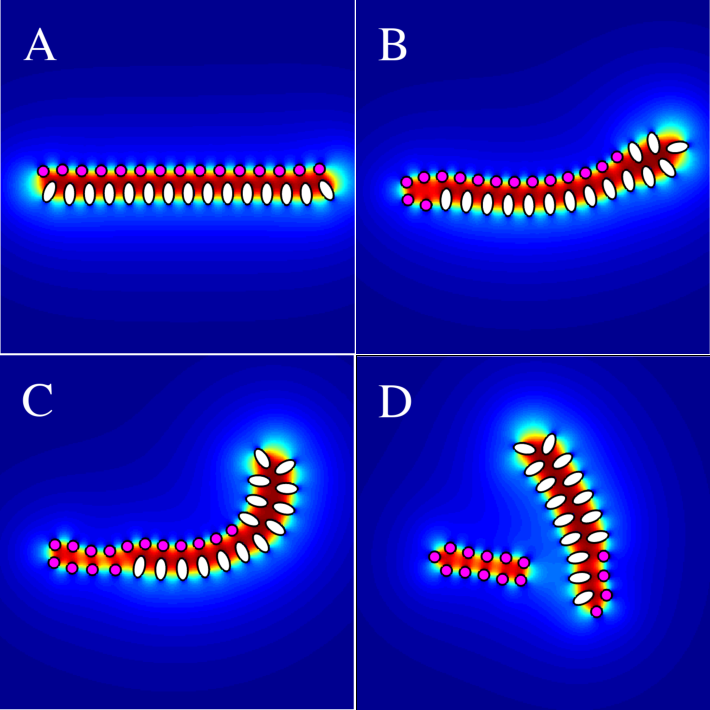
\includegraphics[width=0.4\textwidth]{figures/PW_fig2.pdf}}
%\caption{\label{fig:demixing} An initial assembly of small and 
%large particles spontaneous segregates into two smaller bodies. }
%\end{wrapfigure}
The HAP simulations show vesicle tank-treading. Under the external shear flow, the initially circular 
vesicle rotates in the clockwise direction. As the rate of rotation increases, the vesicle approaches
a steadily tank-treading ellipse. In Figure \ref{fig:tanktreading}B-D, the solid curves are ellipses fit to the particle centers
and midplane respectively. In the non-dimensionalized system, the particles have diameter 2, on the order of $\rho,$ 
and the vesicle diameter is about 14. 
%\todo[inline]{missing units. nm?}
%
\begin{wrapfigure}[12]{r}{0.2\textwidth}
\centerline{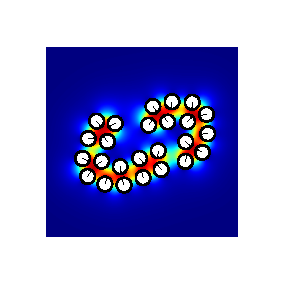
\includegraphics[width=0.2\textwidth]{figures/PW_fig5.pdf}}
\caption{\label{fig:rupture} Rupture of tank-treading vesicle under strong shear flow.}
\end{wrapfigure}
%
Figure~\ref{fig:tanktreading}E shows the aspect ratio of the major to minor axes reaching an equilibrium value in the 
red and blue curves, yet oscillating in the high-shear rate (yellow) curve.
The tank-treading vesicle elongates and becomes more horizontal 
with an increase in flow rate or 
with a decrease in stiffness (effected by decreasing $\rho = 4$ to $\rho = 2$). 


For large shear flow rates, there is an increase in arc length. Here arc length
refers to the the mid-plane circumference. Thus,
some of the external force is going into stretching the vesicle--the other
part is going into bending and viscous dissipation. From our experiments, 
we find that the vesicle ruptures once stretching exceeds about 5 \%
(see Figure \ref{fig:rupture}).
Finally, movies of the tank-treading motion show a slip velocity
between the outer and inner leaflets Figure \ref{fig:tanktreading}G. We have illustrated this 
by tracking the distance between two reference particles in the inner and outer leaflet
(Figure \ref{fig:tanktreading}B \& D, green and blue particles). 
With moderate shear rates or greater adhesion, the particle pair moves in tandem
(in Figure \ref{fig:tanktreading}H, blue and red curves, their distance is more or less constant). 
For a large shear rate, the particle separates as the two leaflets slide against one another. 



%\begin{wrapfigure}[12]{r}{0.2\textwidth}
%\centerline{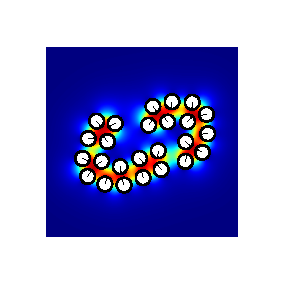
\includegraphics[width=0.2\textwidth]{figures/PW_fig5.pdf}}
%\caption{\label{fig:rupture} Rupture of tank-treading vesicle under strong shear flow.}
%\end{wrapfigure}
There are a number of advantages to using our particle based approach.
For one, the HAP theory automatically accounts for the existence of multiple phases. 
For example, we can vary lipid length, spontaneous curvature and bending rigidity 
by introducing differentiating particle shapes and hydrophobic boundary conditions (Figure \ref{fig:demixing}).
Continuum theory deals with multiple phases through additional surface densities that must
then satisfy specialized transport equations \cite{Lowengrub07,MikuckiZhou17}. 
As illustrated in Figure \ref{fig:tanktreading}, the particle
based approach supports inter-leaflet slip, and this can be used to determine inter-leaflet
and in-plane shear viscosities. 
%





\section{Proposed Research}
\label{sec:proposed-work}
%The proposed research develops fast,
%high-order-accurate, parallel numerical algorithms for large-scale
%simulations of the collective hydrodynamics of amphiphilic particles in a viscous solvent.
%%
We have demonstrated that our hydrophobic attraction with repulsion
potential (HAP) approach efficiently simulates self-assembly of
amphiphilic particles into two-dimensional micelles, bilayer membranes,
and vesicles \cite{Fu2018_SIAM} and recreates the tank-treading
phenomenon in external shear flows \cite{FuQuRyYo20}.
While the results show great promise in the field of collective body
hydrodynamics, several outstanding issues need to be addressed. These
include a thorough analysis of elastic properties of our coarse-grained
bilayers and efficiently simulating three-dimensional collective
hydrodynamics of amphiphilic particles.
We must also incorporate electric charge and account
for how external fields control particle self-assembly. 
%mathematically
%characterize the variational behavior of HARP under appropriate
%homogenized limits.

\subsection{Specific Aim 1: Measuring material properties of amphiphile self-assembly}
\label{subsec:specific_aim_1}

%\begin{figure}
%\begin{center}
%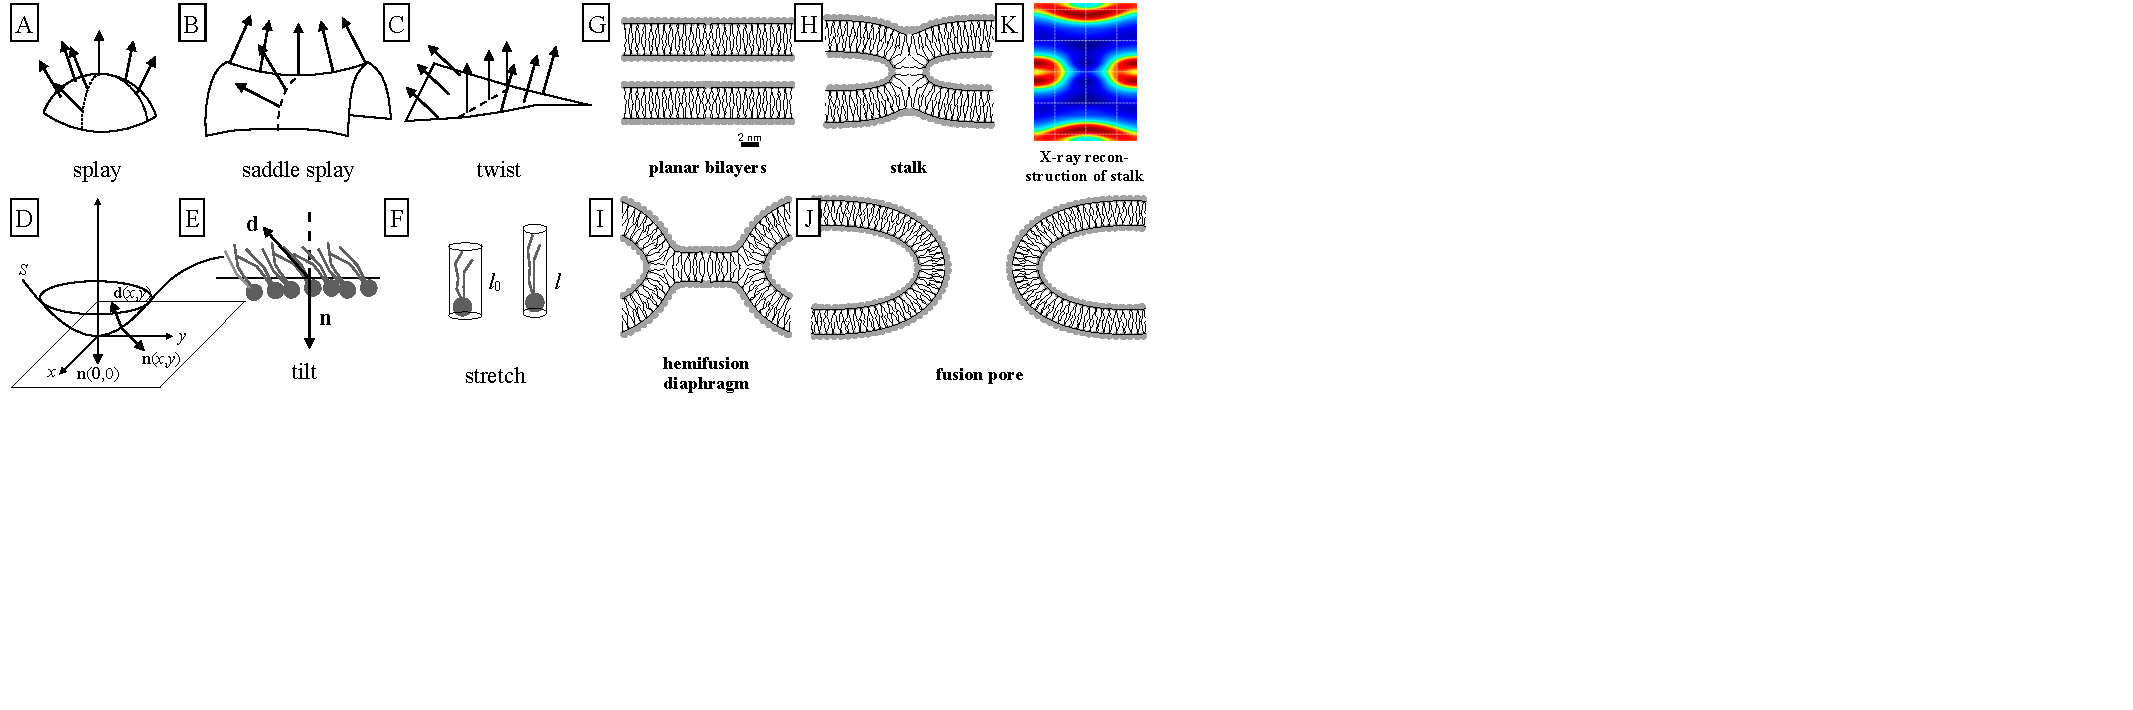
\includegraphics[width=0.9\textwidth]{figures/SA1_fig1.pdf}
%\end{center}
%\caption{\footnotesize (A--C) The splay ($\Div \mathbf{d}$), 
%saddle splay ($\det \mathsf{D}$) and twist ($\Curl \mathbf{d}$) elastic distortions of 
%a monolayer. (D) The monolayer neutral surface $\Sigma$,  
%director $\mathbf{d}$ and unit normal $\mathbf{n}$ in local coordinates.
%(E--F) Lipids are able to tilt from  the surface normal, and stretch.
%(H--J) Intermediates of membrane fusion and (K) experimental image of a stalk \cite{Aeffner2012}. }
%\label{fig:distortions}
%\end{figure}
The goal of Specific Aim 1 is to characterize the material properties of many-body, self-assembled amphiphiles.
For amphiphiles assembled into bilayers, these properties are described by membrane continuum mechanics.
Our goal is to map the parameters of the particle-based model onto the elastic moduli from continuum theory.
Results from this goal will facilitate simulators to use the hydrophobic attraction force calculations
to model bilayers with specific composition. These calculations have provably less computational complexity than
those of molecular dynamics simulations and possess the molecular granularity lacking from continuum models.

Hamm and Kozlov (HK) pioneered 
the modern theory of membrane continuum mechanics \cite{Hamm2000}, and their theory
%was pioneered by Hamm and Kozlov (HK) \cite{Hamm2000}. The theory 
is widely used to describe biological phenomena, including 
fission \cite{FrEsAkSh15, Maetal15, PhysRevE.79.031926},
fusion \cite{ChKo08, KoKo2002,Kuzmin7235,Aeffner2012},
poration \cite{Gaetal20}, phase boundaries, and interaction with inclusions
\cite{SeLeMaEg17,Saetal20, Pietal20}. These phenomena
require resolution of the internal structure of the membrane.  
Recently, there has been a revival in interest in the HK theory as the quadratic assumption
for the elasticity energy density has caused
researchers to question the applicability of the theory 
for large curvatures
\cite{PhysRevLett.117.188102, ARGUDO20161619}.
%
\begin{wrapfigure}[11]{l}{0.47\textwidth}
\centerline{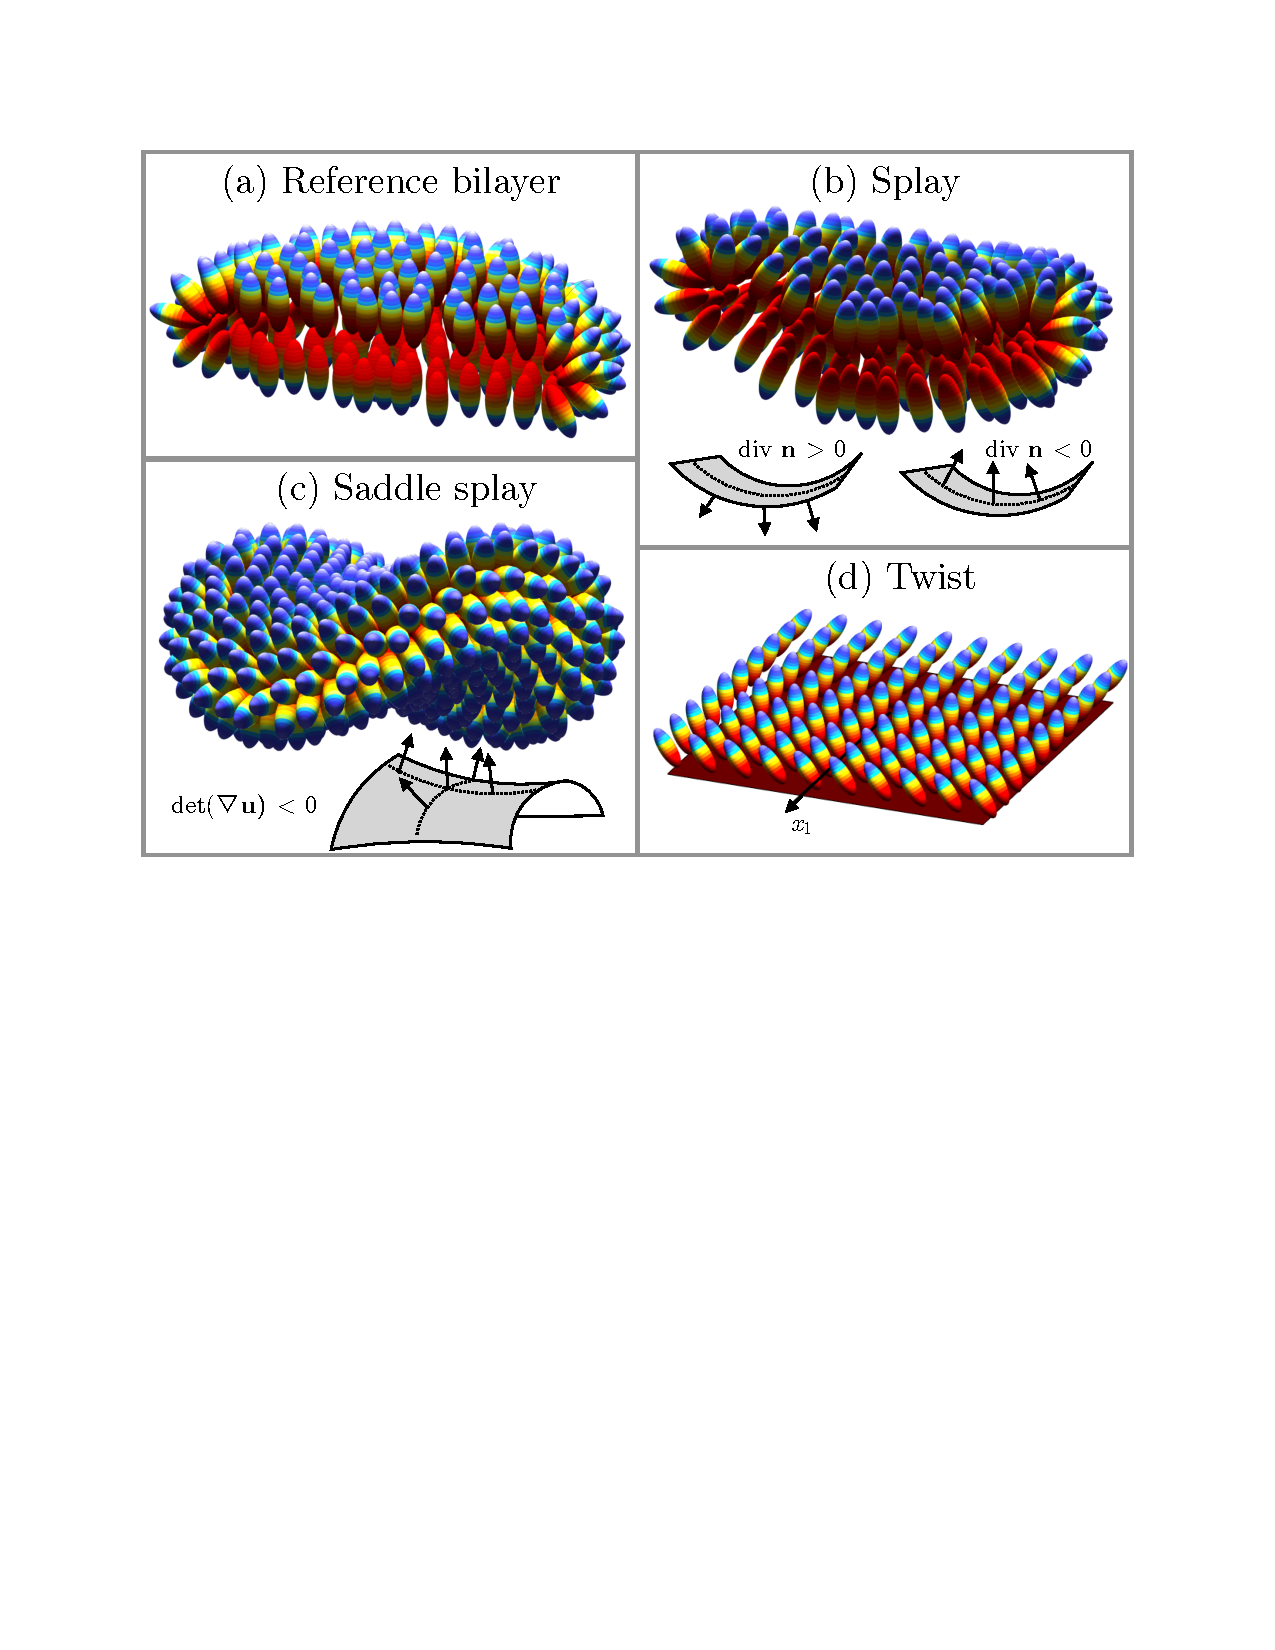
\includegraphics[width=0.47\textwidth]{Figures/Deformations.pdf}}
%  \centering{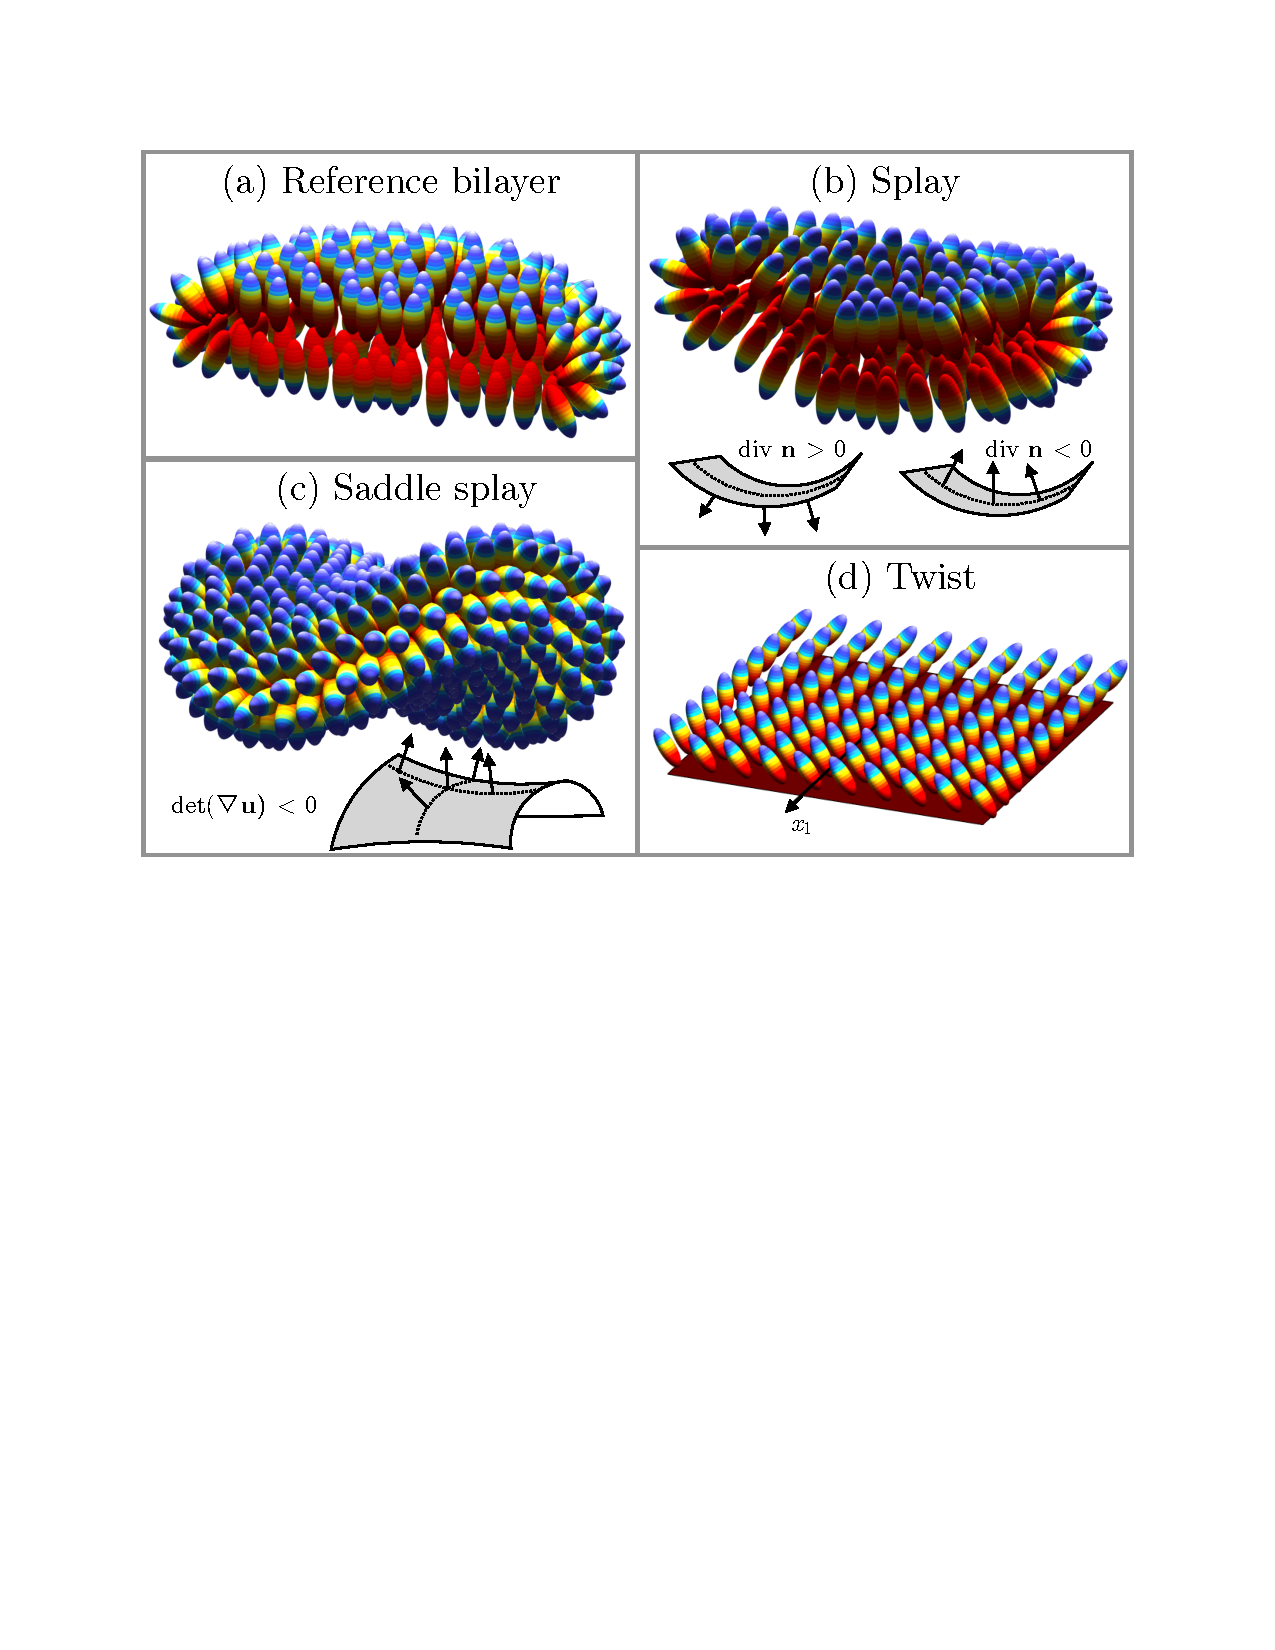
\includegraphics[width=0.80\textwidth]{Figures/Deformations.pdf}}
  \vspace{-5pt}
\caption{\label{fig:deformations} \footnotesize Sketch of the HK
 membrane model \cite{Hamm2000}.}
\end{wrapfigure}
%
This proposal will develop much-needed mathematical analysis to resolve
these controversies due to the assumptions in the HK theory. 
%Using the HK  model as a base,
%PI RR and collaborators calculated, for the first time in continuum theory, a least energy path for transitions between planar bilayers, a membrane stalk,
%hemifusion diaphragm and the fusion pore \cite{RyWaCo13,RyKlYaCo16},
%and the energies calculated by these continuum studies (Figure \ref{fig:barriers}A),
%are in agreement with barrier heights derived by molecular dynamics and experimental studies \cite{FrRoPi17}.  



%\begin{wrapfigure}[13]{l}{0.5\textwidth}
%\centerline{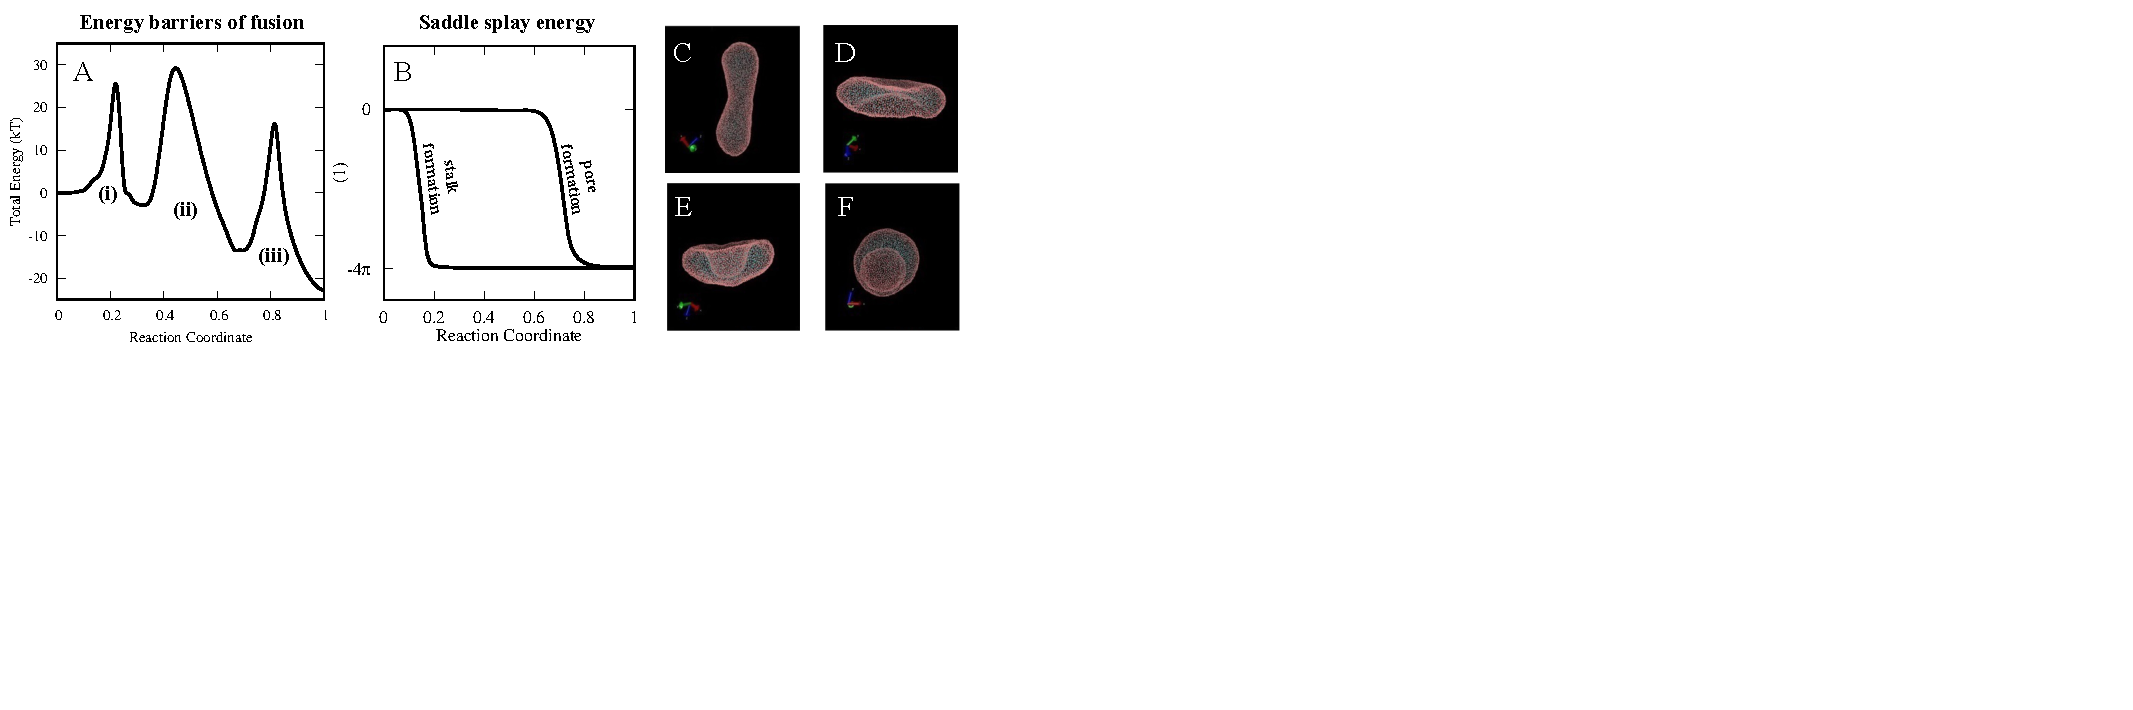
\includegraphics[width=0.5\textwidth]{figures/SA1_fig3.pdf}}
%\caption{{\footnotesize (A) Energy barriers for stalk formation (i), hemifusion
%diaphragm expansion (ii) and pore formation (iii). 
%(B) Saddle-splay energy for each change in \emph{monolayer} topology
%calculated in \cite{RyKlYaCo16}. (C)--(F): Shape transition of vesicle at different values of volume to area ratio from coarse-grained simulations of lipid bilayer membranes \cite{Fu16}.}}
%\label{fig:barriers}
%\end{wrapfigure}

The HK framework assumes a three-dimensional lipid monolayer where the internal structure
consists of straight fibers that represent elongated hydrocarbon chains.
The elastic energy density ${\cal W}$ is quadratic in the Green-Lagrange strain
tensor for this striated, internal structure.
%
%
%
%These fibers
%tilt and stretch with respect to the dividing surface--the surface formed lying between the hydrocarbon chains and polar heads of lipids.
%Accordingly, the deformation takes the form 
%\begin{equation}
%  \label{LMdeformation}
%{\bf x}(X_1, X_2, X_3) = {\bf x}_0(X_1, X_2) + \zeta(x_0(X_1, X_2), X_3) {\bf n}(x_0(X_1, X_2))
%\end{equation}
%where $(X_1,X_2,X_3)$ are points in a reference volume.
%The map $x_0$ parametrizes the dividing surface $\Sigma$, and the unit vector field ${\bf n}$ parametrizes the
%direction of the lipid tails in the deformed state \cite{doi:10.1021/jp075641w,KLAUDA20083074}.
%The parameter $X_3$ and the function $\zeta$ parametrizes the distance along the hydrocarbon chain in the reference state
%and the deformed state, respectively, and so $0 \leq X_3 \leq \delta$ where $\delta = $ 2.5 nm is a realistic monolayer thickness. 
%
%The elastic theory assumes an energy density that is quadratic in the Green-Lagrange strain tensor for ${\bf x}$. 
%The chains stretch and compress to satisfy incompressibility.
%Symmetries with respect to mirror reflection and in-plane rotation, the internal structure assumptions and incompressibility
%lead to an elastic surface energy over the dividing surface $\Sigma$. 
%
This energy density decomposes into four, fundamental, and independent
deformations (Figure~\ref{fig:deformations}): splay ($\Div {\bf n}$),
twist ($\Curl {\bf n}$), saddle splay ($\det \nabla {\bf n}$), and tilt
${\bf t}={\bf n}/({\bf N}\cdot {\bf n}) - {\bf N}$ where ${\bf N}$ is
the unit surface normal;
\begin{equation}
\label{ansatz3}
{\cal W} \equiv \int_{\Sigma} 
  \tfrac{1}{2}\KB\left[ \left( \Div {\bf n} + k_0\right)^2 - k_0^2\right] 
+ \tfrac{1}{2}\KT (\Curl {\bf n})^2 + \KG  \det \nabla {\bf n} + \tfrac{1}{2}\KTH |{\bf t}|^2 \,dA.
\end{equation}
Here, 
%$(\nabla {\bf n})_{ij} = \partial_{x_j}{\bf n} \cdot {\bf e}_i$ is the surface gradient with
%orthonormal tangent vectors $\{{\bf e}_1, {\bf e}_2\}$.
%%\todo[inline]{YNY and BQ: What do you call a coordinate system where the metric is the identity at one point?}
%Also, the surface divergence 
%$\Div {\bf n}$ is the trace, and the surface curl $\Curl {\bf n}$ is the anti-trace (sum of the off-diagonal elements), of $\nabla {\bf n}$ respectively.
%respectively (Figure \ref{fig:distortions}A--C).
the deformations come with elastic coefficients: the bending modulus
$\KB$, twist modulus $\KT$, saddle-splay modulus $\KG$, and tilt modulus
$\KTH$.
%HK define the tilt vector ${\bf t} = {\bf n}/({\bf N}\cdot {\bf n}) - {\bf N}$ where ${\bf N}$ is the unit surface normal.
%
The parameter $k_0$ is the spontaneous curvature and determines the
preferred lipid splay~\cite{RoLi15,Kozlov2007}.  
%As an illustration, the
%lipid DSPC has $k_0 = -0.1$ nm$^{-1}$ 
%%as a result of  %having a relatively long acyl chain. 
%and these lipids would preferentially line the upper monolayer in Figure \ref{fig:deformations}B  
%because the addition of a positive splay 
%to the negative spontaneous curvature leads to lower energy \cite{Kamal22245, C3SM51829A, RoLi15,FriedSeguin15}.
%The subtraction of $k_0^2$ makes the energy distortion free
%\cite{Helfrich73,PhysRevLett.113.248102,Hamm2000}.

Although the HK elastic theory assumes small deformations, 
Galimzyanov {\em et al.}~\cite{C9SM02079A} have shown that energies derived from
molecular dynamics and those derived from \eqref{ansatz3} are in agreement, even when curvatures are large.
Under spatial scales much larger than the
membrane thickness, membrane energy is well-characterized by the
Canham-Helfrich energy used throughout the fluid-structure literature
\cite{QiangDu09, Lowengrub07,KimLai2010_JCP, Hu, HuLaiSeolEtAl2016_JCP, qua-bir2014, qua-vee-you2019}.
%\todo[inline]{YNY: place your recent works here}
The Canham-Helfrich energy is actually a special case of
\eqref{ansatz3} obtained by setting ${\bf n} =  \pm {\bf N}$ (the $\pm$ depending on
orientation) and collapsing both monolayers onto the membrane midplane.
%There, splay $\Div n$ equal to twice the mean curvature, saddle splay
%$\det \nabla n$ equal to the Gauss curvature, and both twist and tilt
%are equal to zero. 

%\begin{figure}
%\begin{center}
%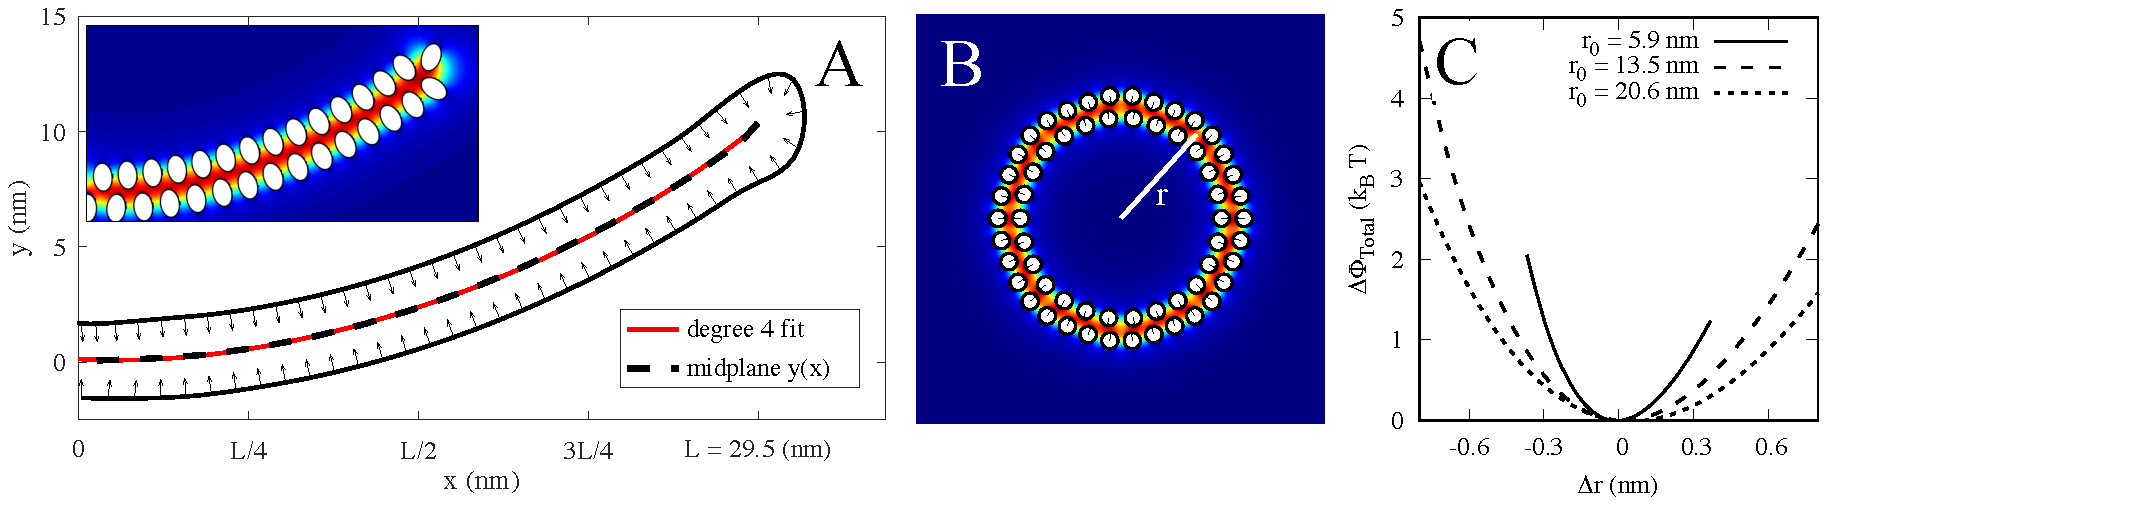
\includegraphics[width=\textwidth]{figures/SA1_fig2.pdf}
%\end{center}\vspace{-1.em}
%\caption{\footnotesize (A) A partially clamped bilayer with mid-plane (dashed curve) under uniform load.
%The quartic fit comes from continuum theory. 
%(B) A circular vesicle at equilibrium. (C) The area modulus derives
%from convexity in energy as a function of radius. 
%\label{fig:bend}}
%\end{figure}


% Proposers should address what they want to do,
% why they want to do it,
% how they plan to do it,
% how they will know if they succeed,
% and what benefits could accrue if the project is successful.
%\begin{center}
%Preliminary results
%\end{center}

%\begin{wrapfigure}[13]{l}{0.5\textwidth}
%\centerline{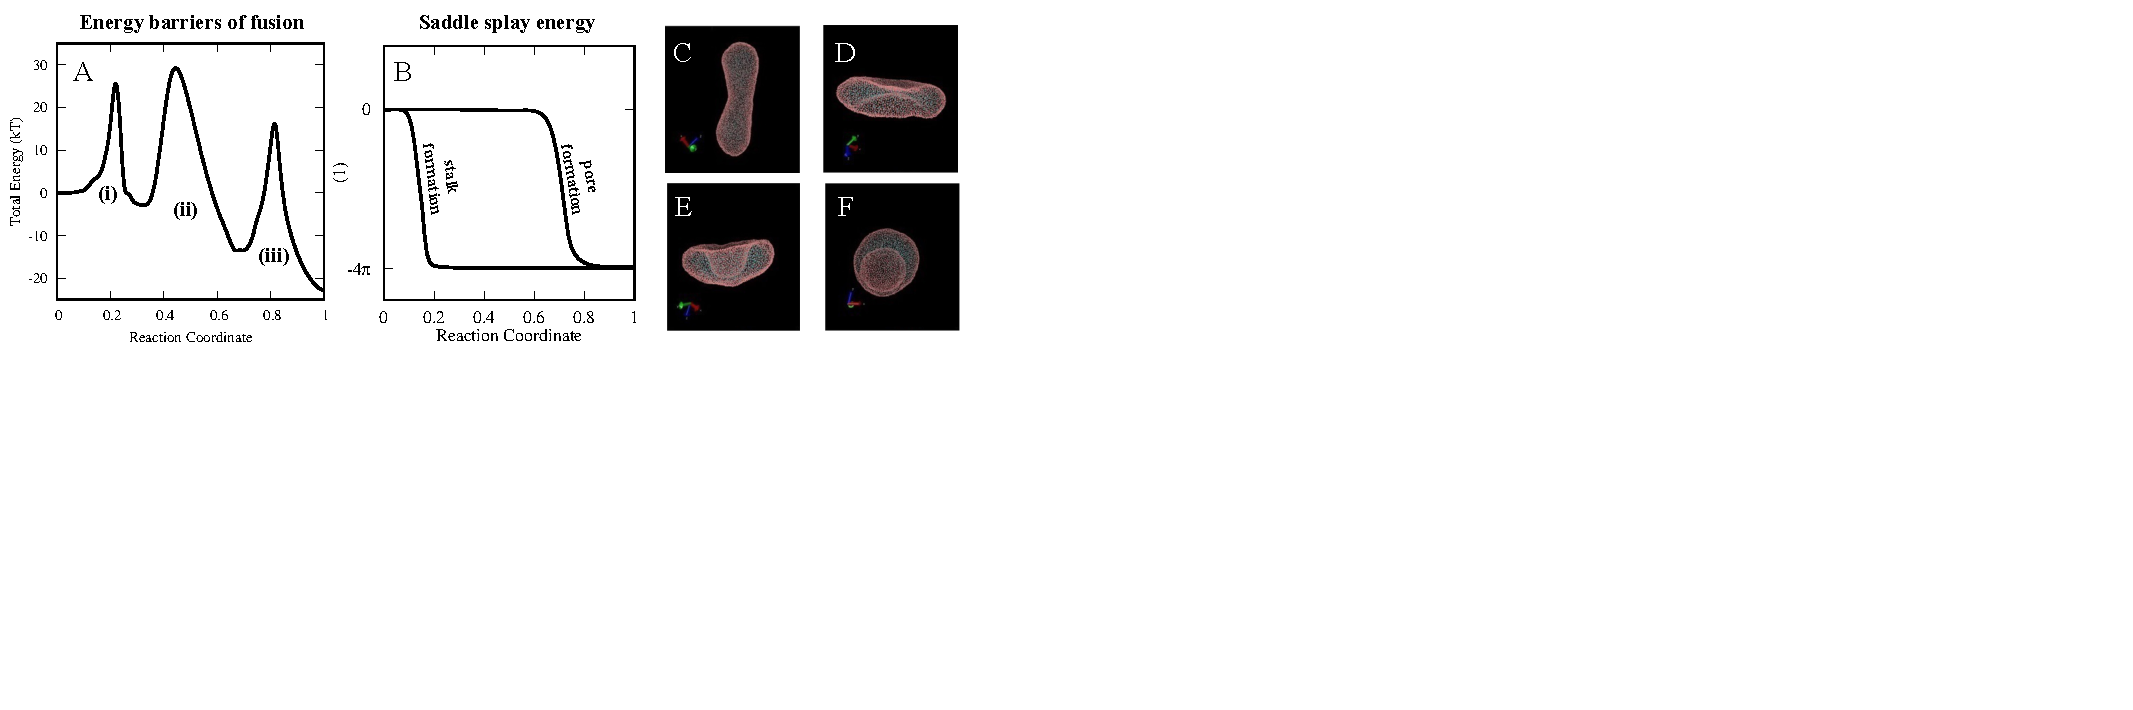
\includegraphics[width=0.5\textwidth]{figures/SA1_fig3.pdf}}
%\caption{{\footnotesize (A) Energy barriers for stalk formation (i), hemifusion
%diaphragm expansion (ii) and pore formation (iii). 
%(B) Saddle-splay energy for each change in \emph{monolayer} topology
%calculated in \cite{RyKlYaCo16}. (C)--(F): Shape transition of vesicle at different values of volume to area ratio from coarse-grained simulations of lipid bilayer membranes \cite{Fu16}.}}
%\label{fig:barriers}
%\end{wrapfigure}

%\begin{center}
%Anticipated model simulations
%\end{center}
\subsubsection{Simulations of the HARP model to estimate elastic moduli and energy}
%To characterize material properties of a bilayer, we compare the energies and forces generated by
%a collection of amphiphilic particles against the energies and forces of a continuum bilayer.
We propose to
%
%to examine conduct calculations similar to the example of figure~\ref{fig:flattening}
%for a wide range of particle parameters and physical parameters in HARP to 
%
%{\bf (i)} Assess whether the continuum energies \eqref{ansatz3} are the same
%as the corresponding energies in the particle system for all reasonable deformation.
%If this is the case we will 
%
{\bf (i)} determine the value of effective elastic moduli $\KB$,
$\KT$, $\KG$, and $\KTH$ and then {\bf (ii)} understand how the model parameters $\rho,$ $\gamma$, and
particle shape map onto elastic moduli. 
An accurate and robust way to measure material properties is to track the evolution of the bilayer as
%
\begin{wrapfigure}[10]{r}{0.4\textwidth}
\vspace{-0.3cm}
\centerline{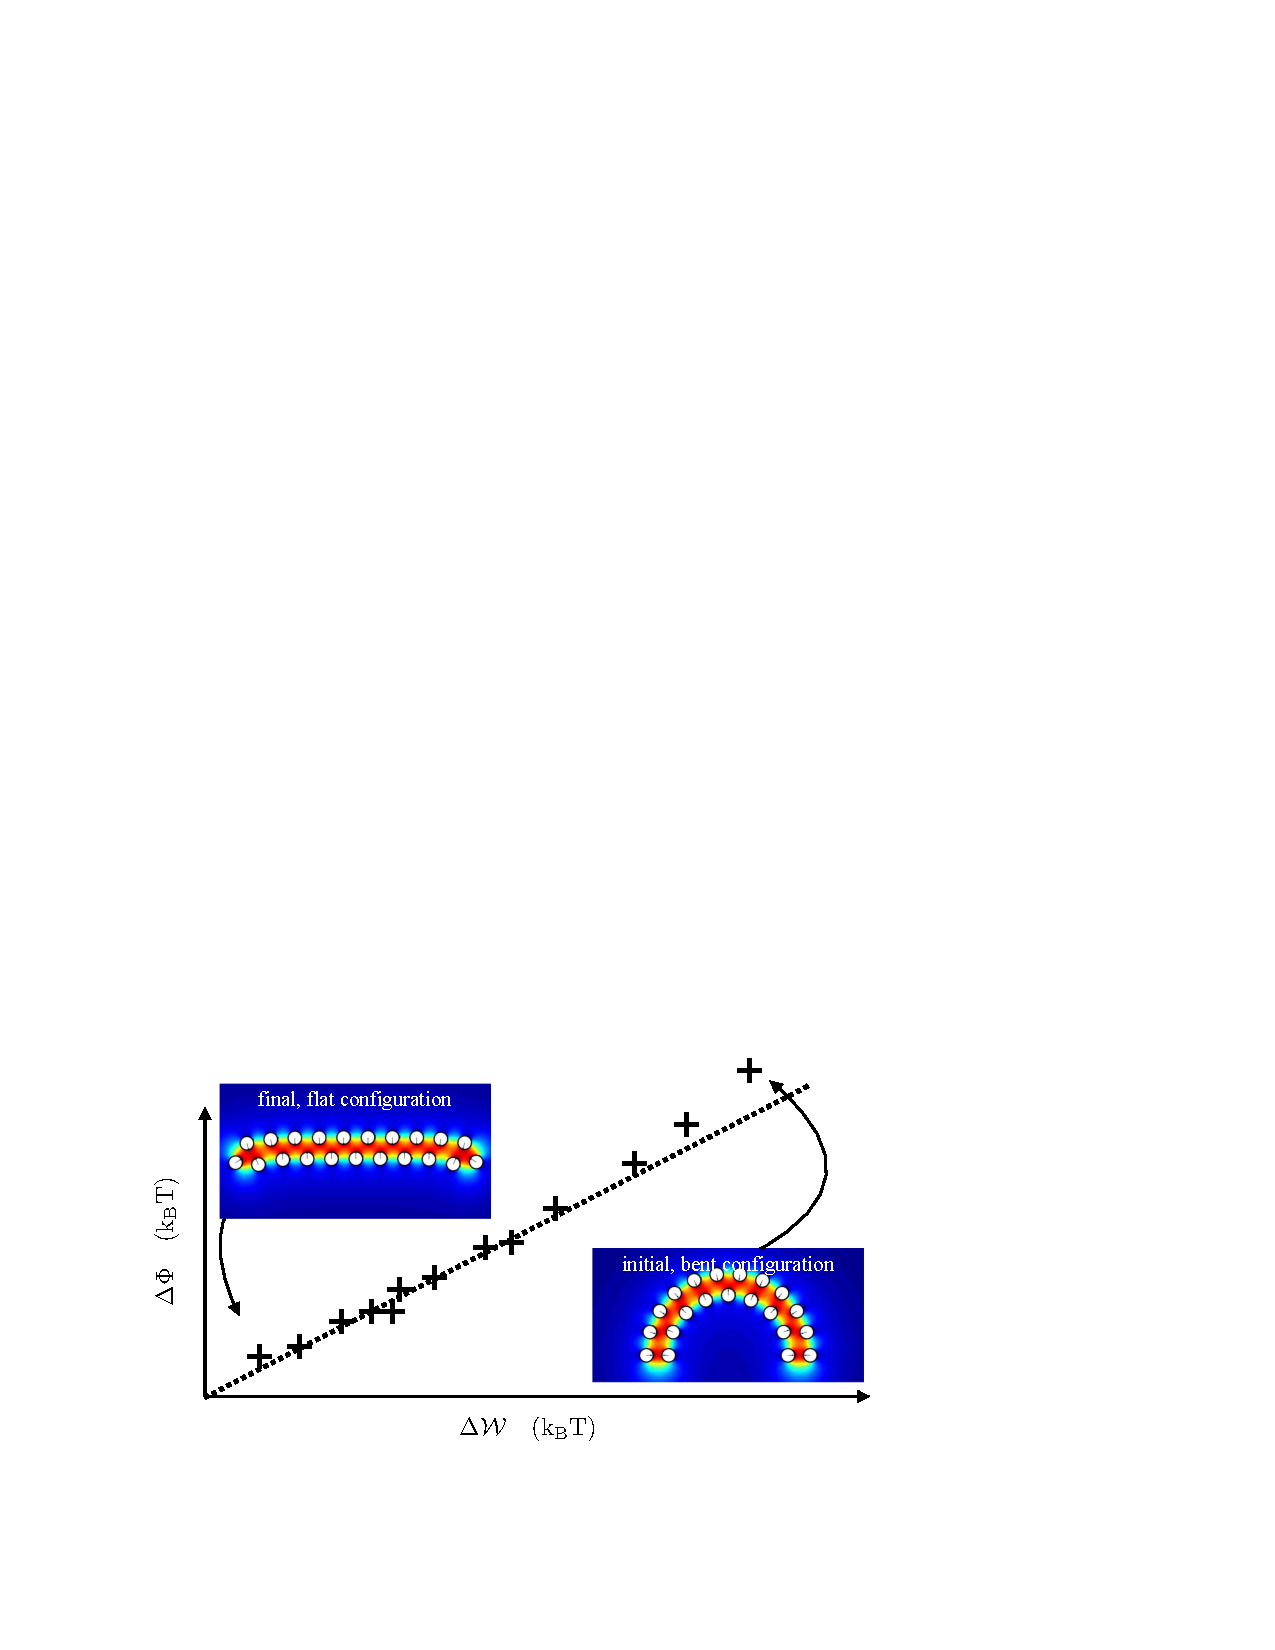
\includegraphics[width=0.4\textwidth]{Figures/Flattening.pdf}}
%  \centering{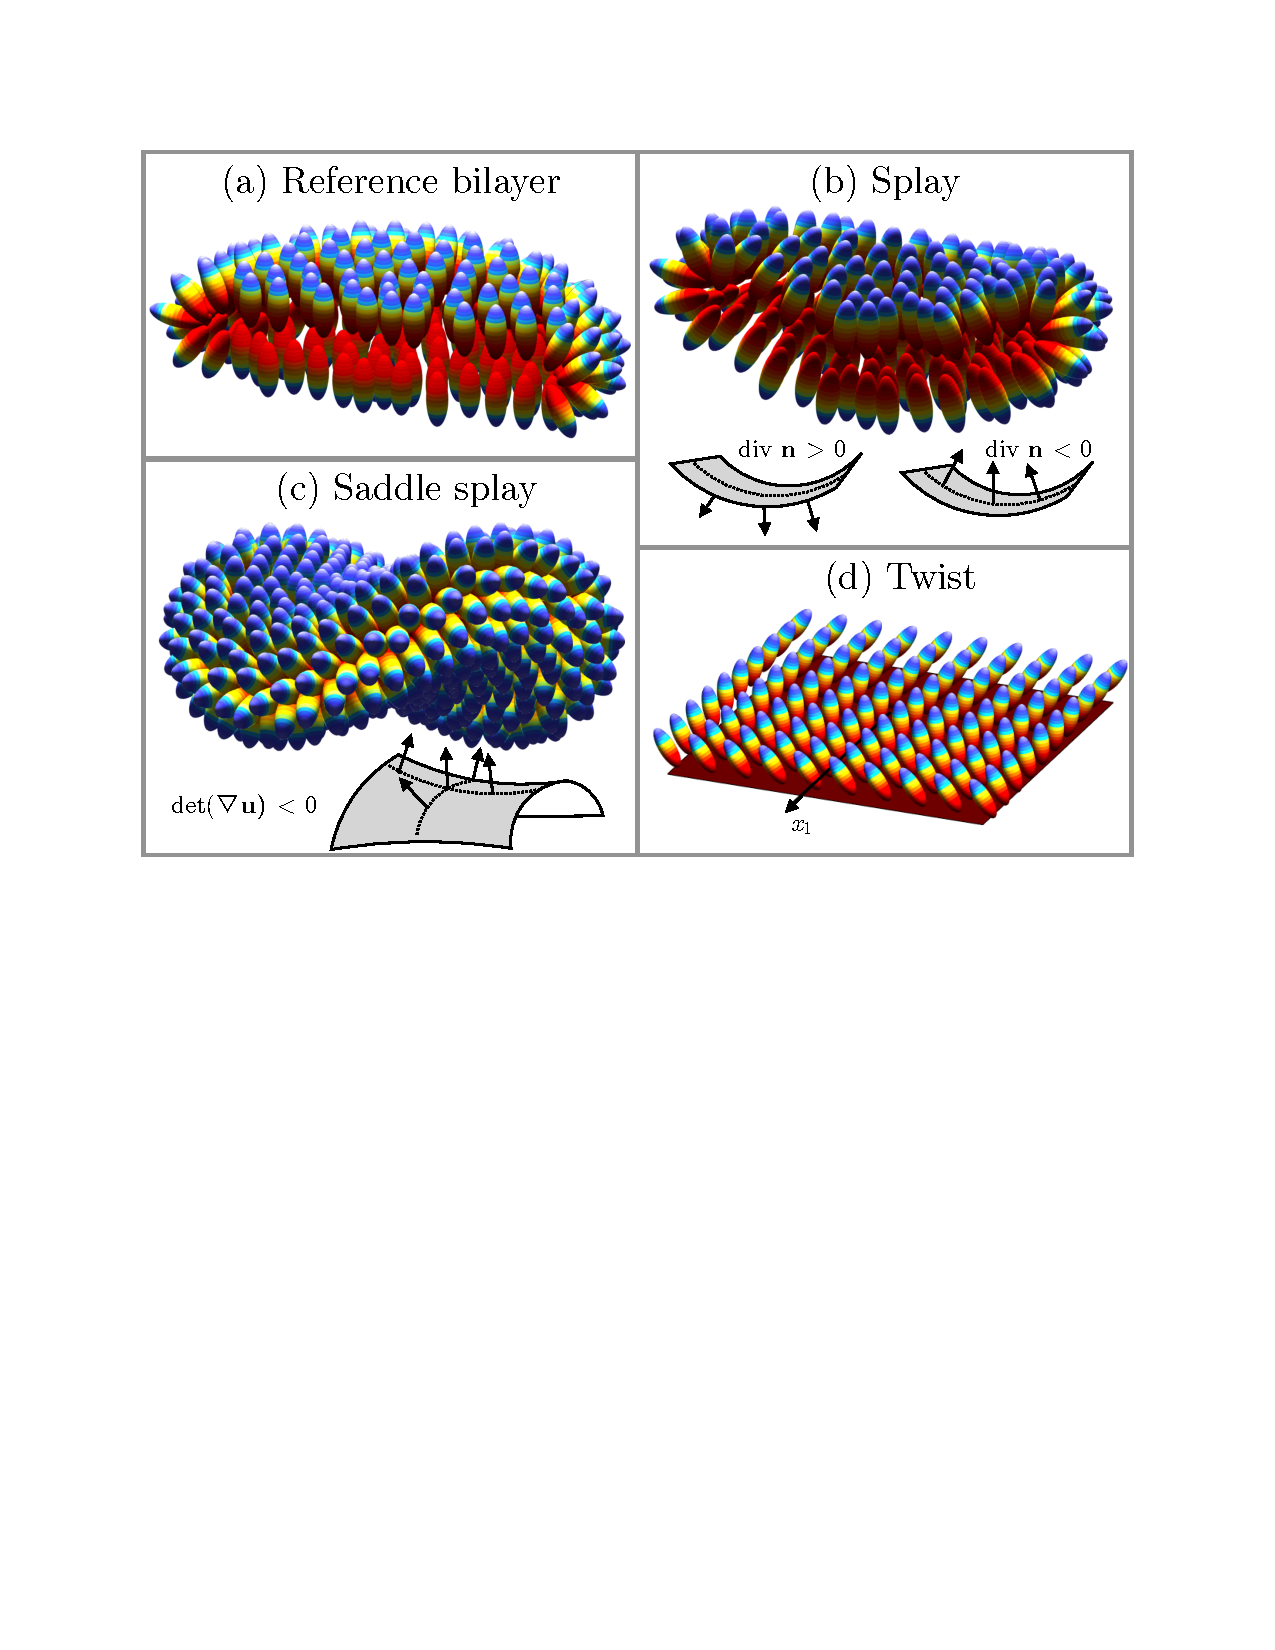
\includegraphics[width=0.80\textwidth]{Figures/Deformations.pdf}}
\vspace{-0.2cm}
\caption{\label{fig:flattening} \footnotesize Example of computing
  bending modulus of a lipid bilayer from particle simulation.}
\end{wrapfigure}
it relaxes from an initially non-equilibrium
configuration~\cite{PhysRevLett.117.188102}. Figure~\ref{fig:flattening}
shows an example where the initial configuration of a lipid bilayer
patch contains only splay deformation without any other components
(saddle splay, twist and tilt). As the bent membrane flattens, we find
that both the membrane self-interaction energy $\Phi$ and the elastic
energy ${\cal W}$ decrease, and because the saddle splay, twist, and
tilt stay zero, the slope gives the bending modulus in this case. 

%To characterize material properties of a bilayer, we compare the energies and forces generated by
%a collection of amphiphilic particles against the energies and forces of a continuum bilayer.
%We propose to first {\bf (i)} Assess whether the continuum energies \eqref{ansatz3} are the same
%as the corresponding energies in the particle system for all reasonable deformation.
%If this is the case we will {\bf (ii)} determine the value of the elastic $\KB$,
%$\KT$, $\KG$ and $\KTH$, and then {\bf (iii)} understand how the model parameters $\rho,$ $\gamma$, and particle shape map onto elastic moduli. 
%%
%%Motivated by our preliminary results \cite{Fu2018_SIAM}
%%we use realistic values for particle diameter $2$ nm \cite{Boal},
%%screening length $\rho = 2.5$ nm \cite{Eriksson1989,Lin2005,Parsegian,Israelachvili80,TerziDeserno17}
%%and interfacial tension $\gamma=4.1$ pN nm$^{-1}$ \cite{GarciaSaez, KUZMIN2005, Petelska2012, Jackson}
%%model parameters. The repulsion strength, repulsion length scale, particle shape (e.g. disks, ellipses), 
%%particle diameter and the hydrophobic boundary condition \eqref{SL}
%%are additional parameters defining the coarse-grained representation. 
%
%An accurate and robust way to measure material properties is to track the evolution of the bilayer. 

Here we start with a particle-based bilayer in a specific non-equilibrium shape that involves only one of the components of the displacement in Figure~\ref{fig:deformations}, and then evolve the particle system according to the time integration for \eqref{eq:stokes}.
Because elastic properties are independent of dissipation,
we can forgo solving for fluid velocity and set the translational
velocity and angular velocity directly proportional to force and torque. 
%bilayer by steepest gradient descent 
%with respect to the HARP functional:
%\begin{equation}
%\label{SGD}   
%\frac{\dif {\bf a}_i}{\dif t} = {\bf F}_i,    \quad  \frac{\dif {\bf R}_i}{\dif t}  = {\bf R}_i A({\bf w}_i),\quad i = 1, \dots, N.
%\end{equation}
%where that particle centers ${\bf a}_i$ and rotation matrices ${\bf R}_i$ determine the particle configuraton; %
%$A({\bf w}_i)$ is the skew-symmetric matrix with axial vector ${\bf w}_i$.
%We solve \eqref{SGD} numerically  using an Adams–Bashforth linear multistep method. 
%The procedure involves solving \eqref{SL} based off of the current particle configuration.
%We then use the solution $u$ to calculate the collection of forces and torques \eqref{forceandtorque}, and update the particle configuration
%through \eqref{SGD}.
%
\begin{wrapfigure}[11]{l}{0.32\textwidth}
\centerline{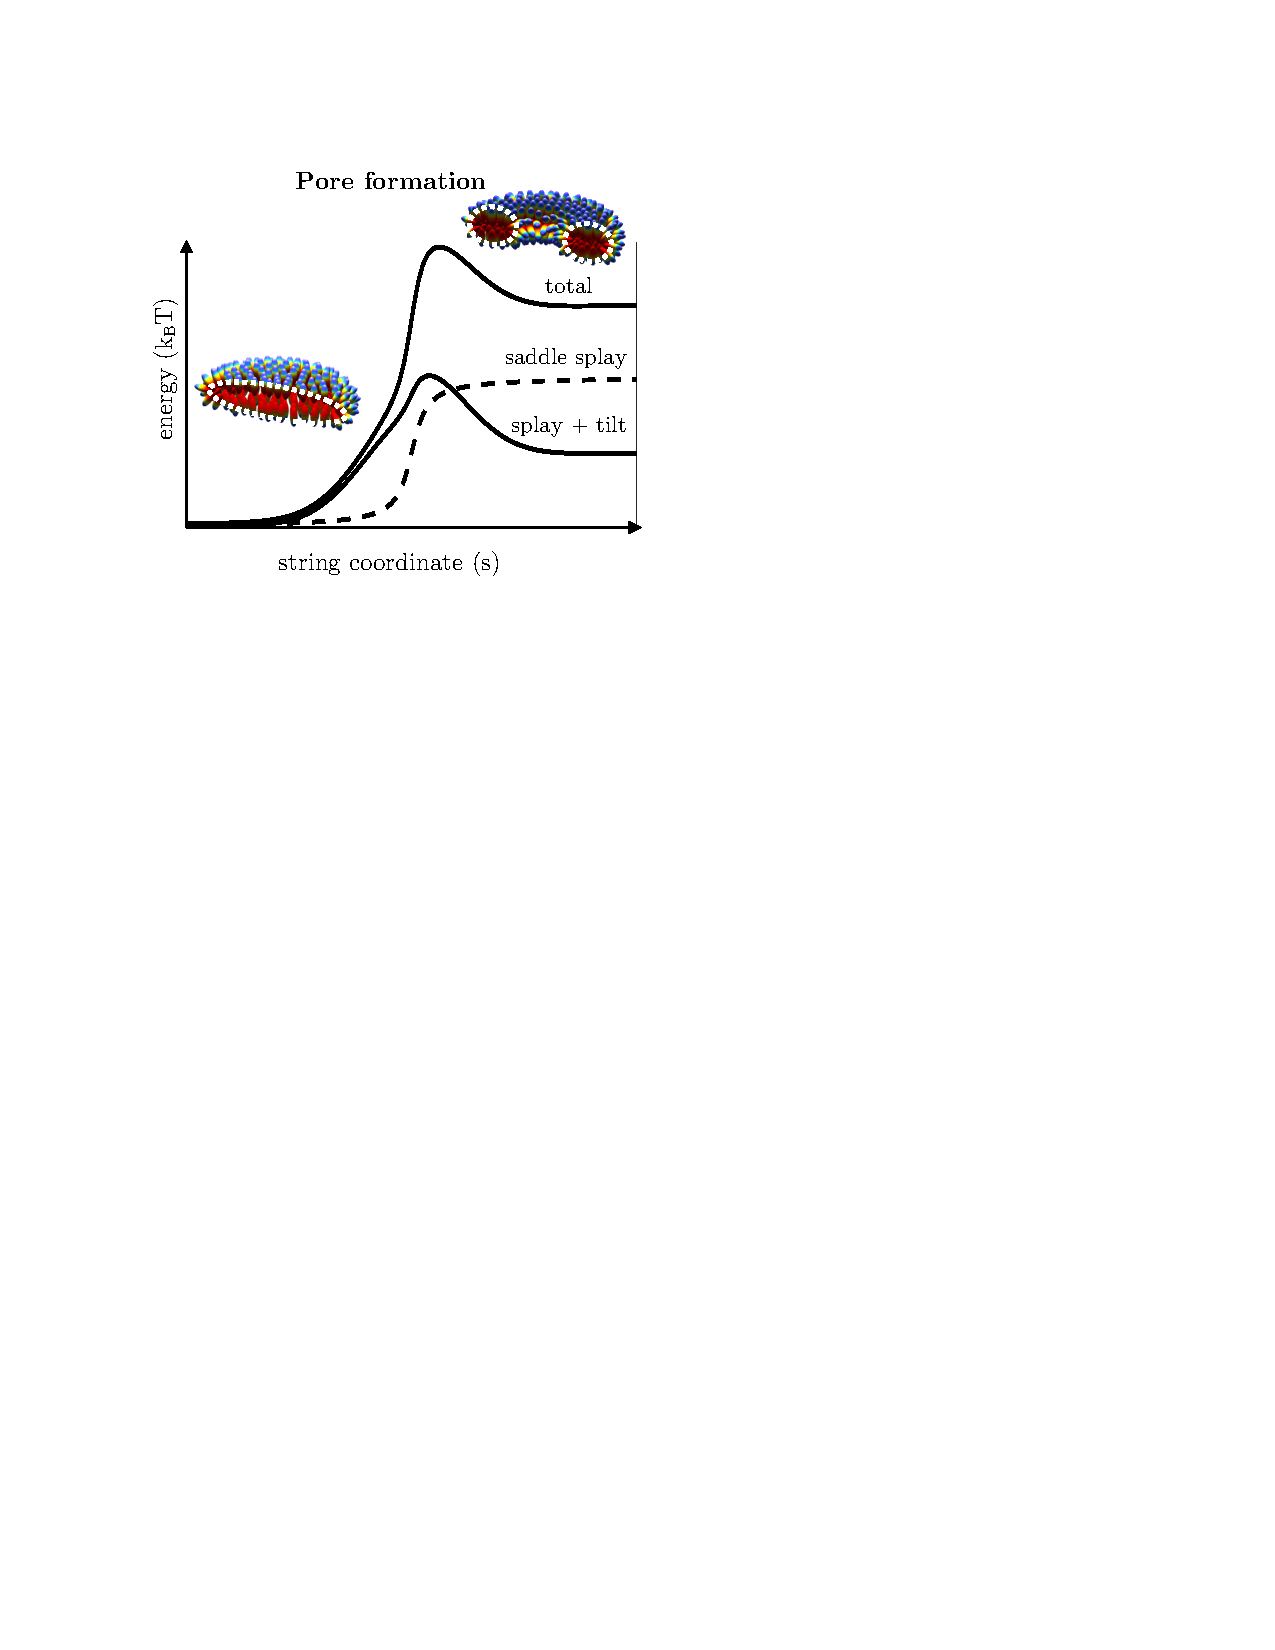
\includegraphics[width=0.32\textwidth]{Figures/SaddleSplayDiagram.pdf}}
  \vspace{-8pt}
\caption{\label{fig:saddle_splay} \footnotesize Example of determining the
  saddle splay modulus.}
\end{wrapfigure}
%
This yields a dissipation of the total potential \eqref{eq:total_poten}, which
stabilizes the evolving bilayer shape.
Therefore, we reconstruct an evolving monolayer dividing surface $\Sigma$ and director field ${\bf n}$ by
interpolating the particle centers and orientations. Using \eqref{ansatz3}, we calculate a continuum energy $\mathcal{W}$ from the interpolated shapes.

%In certain instances, the bilayer evolution involves only one or a few of the four fundamental deformations.
%When this occurs, the elastic moduli derive from the coefficients of the linear regression between the HAP energy $\Delta \Phi = \Phi - \Phi_0$
%and continuum energies and $\Delta E = E - E_0$, where  $\Phi_0$ and $E_0$ are respective equilibrium values.

%
%Since it is a particle-based method, the HAP model has a number of advantages over continuum-based descriptions.
%The elastic energy \eqref{ansatz3} couples director gradients to surface geometry through
%the tilt vector field.  Furthermore, bilayer energy is the sum of two monolayer
%energies and the distance between these monolayers varies according to \eqref{LMdeformation}.
%Effects like tilt and varying monolayer thickness appear at lipid domain boundaries, the edge of nanopores and at the boundary of membrane inclusions \cite{PhysRevE.102.042406}.
%These effects are present in the proposed formulation, and the particle-based bilayers can break open and join monolayer-wise 
%as required by fussion and fission. 
%
%Bending is the energetically most consequential deformations. To measure a bending modulus,  
%we deform the midplane of a planar bilayer into the shape of a circular arc.
%This arc stores bending energy in the form of splay $\Div {\bf n}$, while twist, saddle-splay and tilt deformations are zero.
%The splay in the two leaflets approximately cancel when added, making the contribution of spontaneous curvature negligible.
%In the case of a rectangular bialyer, the corresponding elastic energy 
%$E = \int_{\Sigma} \KB \kappa^2$ where $\kappa$ is the curvature of the curved cross-section $C$.
%Figure \ref{} shows the approximately linear relationship between $\Delta \Phi$ and $\Delta E$
%used to values for infer $\KB$. 

We propose to conduct calculations similar to the example of Figure~\ref{fig:flattening}
for other elastic moduli such as the effective twist modulus $\KT$.
Molecular dynamics investigations find a twist modulus about 1
\kBT~\cite{LeVeWa14}, and here, the specific non-equilibrium shape consists of
a single layer of amphiphilic particles on a hydrophobic substrate as
illustrated by Figure~\ref{fig:deformations}D. Having a nonzero twist
requires nonzero tilt because the surface gradient of the lipid
director equals the second fundamental form
%, and is therefore symmetric,
whenever tilt is zero locally. The twist deformation is a fully
three-dimensional deformation. \S\ref{subsec:specific_aim_3} addresses outstanding implementation issues like three-dimensional boundary integral equation solvers.

%for a wide range of particle parameters and physical parameters in HARP to 
%
%We will also determine the effective saddle splay modulus $\KG$. 
The gradient descent technique is ineffective for measuring the saddle splay modulus $\KG$ because
the saddle splay energy is largely invariant under shape changes.
To evaluate $\KG$, we will combine the present particle simulations with the string method 
from PI RR's work on membrane fusion \cite{RyKlYaCo16}. The string method is a numerical scheme that finds
least energy pathways separating energy basins \cite{doi:10.1063/1.2720838}. 
In the simplified Canham-Helfrich formulation, saddle splay energy is an exact indicator of topological transitions, 
thanks to the  Gauss-Bonnet theorem \cite{TerziDeserno17}.
More generally, PI RR has shown that saddle splay acts as a topological indicator even in the presence of nonzero tilt \cite{RyKlYaCo16}. 
As a result, saddle splay can be quantified from the transition energies of a least energy path of pore formation (Figure \ref{fig:saddle_splay}).   
%Using the string method, we will evaluate the transition energies between the intact pancake shape,
%and one with a pore. Pore formation in a single bilayer decreases the integral of saddle splay from $4\pi$
%to $0$. We can, in principle, detect this drop in energy because we have already accounted for the other deformations. 
%
%%We will also analyze $\KG$ using a helical geometry. In a helicoid with inclination $m$, the director
%%gradient is $\nabla n = \begin{pmatrix} 0 & m(m^2+x_1^2)^{-1} \\ m(m^2+x_1^2)^{-1} & 0\end{pmatrix}$ where $x_1$ is the distance to the central
%%axis. We observe that saddle splay, twist and tilt are zeros, and $\det \nabla n = m^2(m^2+x_1^2)^{-2}$.
%%In the simulations, the particles forming the helicoid will be confined to two, concentric cylinders. The
%%continuum energy $\tfrac{1}{2}\KG h(m x_1(m^2+x_1^2)^{-1} + \tan^{-1}(x_1/m)) |_{r_1}^{r_2}$ where $h$, $r_1$ and $r_2$
%%are the cylinder heights, inner cylinder radius, and outer cylinder radius, respectively. 
%

%The proposed particle-based simulations of the HARP model in equations~\ref{SGD} also allow direct examination on the assumption of quadratic form of the elastic energy density.
%As discussed earlier, recent disagreement in elastic moduli between continuum model and MD simulations originates from such assumption. 
%The particle-based HARP model provides a unique opportunity to examine the validity of the quadratic elastic energy, and the PIs propose to examine how (if) any deviation from the quadratic elastic energy may depend on the microscopic details of the amphiphilic particles and their interactions.

%\subsubsection{HK elastic energy form}
\noindent{\bf{HK elastic energy form:}}
The field of membrane continuum mechanics still lacks consensus as to whether \eqref{ansatz3} is the appropriate functional for bilayer energy.
\textbf{(i)} Researchers have assumed that $\KT = 0$ to effect lateral fluidity in
membranes~\cite{Hamm2000, TerziDeserno17, C9SM02079A,
PhysRevE.102.042406}. 
A value $\KT = 0$, however, makes \eqref{ansatz3} a noncoercive functional.
%and leads to the nonphysical conclusion that there are bilayers 
%with $\nabla {\bf n} \to \infty$ but $\mathcal{W} \to 0.$ 
\textbf{(ii)} Recently,~\cite{TerziDeserno17} derived a tilt curvature
term that was neglected from the HK analysis~\cite{Hamm2000}.
Later,~\cite{C9SM02079A} and~\cite{PhysRevE.102.042406} independently
identified an inconsistency in the argument used
by~\cite{TerziDeserno17} arising
from a transversal tilt invariance assumption.
In~\cite{RyKlYaCo16}, PI RR and collaborators showed that the tilt vector leads to unphysical cusps depending on how one accounts for membrane thickness.  
\textbf{(iii)} Theoretical analysis of lipid phase transitions predict a
negative saddle-splay modulus around $-8$ \kBT~\cite{SIEGEL2004366,
SIEGEL20085200} that gives rise to a larger energy barrier for
monolayer fusion than is found by experiments~\cite{FrRoPi17, Tran7106,
TerziDeserno17}.
%
%
%Researchers point out, however, that this theoretical value requires a larger energy 
%barrier for monolayer fusion than is found by experiment \cite{FrRoPi17,Tran7106,TerziDeserno17}.
%Furthermore, the stability conditions of \eqref{ansatz3} require $\KG \geq -4\min\{\KB,\KT\}$, suggesting a smaller magnitude for $\KG$.

% The constants $\KB$, $\KT$  and $\KG$ play the same role as the Frank constants $K_1$, $K_2$ and $K_{24}$
% liquid crystal theory. However, the ``bend'' distortion from nematics  
% is not present in monolayers since the directors have no dependence in the normal direction.
% There is also no ``spontaneous twist'' in monolayers due to invariance under mirror reflection. 

The form of the elastic energy density~\eqref{ansatz3} is the same as
the Oseen-Frank energy density for nematic liquid
crystals~\cite{ANDRIENKO2018520, Tran7106, Helfrich73}. In fact, a lipid
monolayer acts as one layer in a smectic phase~\cite{REYESMATEO1995978,
Rangamani20140463, PhysRevLett.113.248102}. Based on this observation,
we propose to examine the HK analysis to resolve the aforementioned
inconsistencies. We will expand the strain tensor in terms of a plane
perpendicular to ${\bf n}$ (instead of the monolayer tangent plane as
done in the past works) so that the gradient terms in the elastic energy
completely decouple. Using this expansion we prove an exact identity
that gives the incompressibility condition by a Steiner-type polynomial
in $\Div {\bf n}$ and $\det \nabla {\bf n}$ \cite{Fe59}. In contrast,
the works~\cite{TerziDeserno17, PhysRevE.102.042406, Hamm2000,
C9SM02079A} utilize an approximate identity for incompressibility as a base,
so we can considerably improve upon the analysis of monolayer energy.

%  Past researchers expressed the strain tensor in terms of monolayer tangent plane.   
%  In this frame, however, there is a coupling between the gradients of the monolayer surface, lipid direction, and chain length,
%  and accounting for these couplings by Taylor expansion  
%  can lead to an energy density with an unruly number of parameters \cite{PhysRevE.102.042406}.
%
%The form of the elastic energy density \eqref{ansatz3} is the same as
%  the Oseen-Frank energy density for nematic liquid crystals \cite{ANDRIENKO2018520,Tran7106,Helfrich73}.   In fact,  
%  a lipid monolayer acts as one layer in a smectic  phase \cite{REYESMATEO1995978,Rangamani20140463,PhysRevLett.113.248102}. 
%  Motivated by liquid crystal theory, we have found that the gradient terms completely decouples when 
%  expanding the strain tensor, not in terms of the monolayer tangent plane, but in terms of a plane perpendicular to ${\bf n}$. 
%  Using this observation, we prove an exact identity 
%  that gives the incompressibility condition by a Steiner-type polynomial in $\Div {\bf n}$ and $\det \nabla {\bf n}$ \cite{Fe59}.
%  In contrast, the works \cite{TerziDeserno17, PhysRevE.102.042406, Hamm2000, C9SM02079A} utilize an
%  approximate identity for incompressibility, and so we can offer a considerably more accurate analysis of monolayer energy.
%  
%%To measure the twist modulus, we place a single monolayer on a hydrophobic substrate 
%%and take the initial configuration ${\bf n} = (0, f(x_1), \sqrt{1 - f^2(x_1)})$,
%%yielding a surface gradient $\nabla {\bf n} = \begin{pmatrix}0 & 0\\ f'(x_1) & 0\end{pmatrix}$. 
%%  Here $\Div {\bf n} = \mathrm{tr}(\nabla {\bf n}) = 0$, $\det(\nabla {\bf n}) = 0$ and
%%  $\Curl {\bf n} = (\nabla u)_{12} - (\nabla u)_{21} = f'(x_1)$.
%%  This gives the continuum elastic energy equals
%%  \begin{equation}
%%    \label{eq:twist_energy}
%%    E = \int_{\Sigma} \tfrac{1}{2}\KT (f'(x_1))^2 + \tfrac{1}{2} \KTH f^2(x_1) \,\dif dx_1 \dif x_2,
%%  \end{equation}
%%  which we compare to the HAP simulation data.
%
\subsubsection{Asymptotic analysis on the limit $\rho\rightarrow 0$ of HAP}
The HAP energy converges to the surface energy in the limit of vanishing screening length~\cite{Shibata2004}.
Also, the boundary layers of the solutions to the screen Laplace equation
converge to area measures supported on the particle boundaries \cite{Lee2018, Lin2015, Shibata2004}.
These phenomena are analogous to the sharp interface limit in the phase-field functional,
and motivate developing the mathematical connections between the HAP energy and
the energy functionals used in the gradient theory of phase transitions.
formulation~\cite{Modica87, MODICA1987487, LuMo89}.
PI RR has worked on phase field approximations of membrane bending
energy~\cite{0951-7715-18-3-016} and asymptotcs in the Poisson-Boltzman
equation~\cite{1531-3492_2006_2_357, Lee2018}.
The screened-Laplace equations~\eqref{SL} is the linearization of the Poisson-Boltzmann equation.
One set of questions is to establish the HAP convergence rate as a
function of particle geometry~\cite{LuMo89}, which can be used as a
benchmark for numerical validation.
Ultimately, we will be able to address the so-called $\Gamma$-convergence of energy minimizing
particle configurations in the zero-decay length limit \cite{Roger2006, Mugnai2013}. 
%The phase field functional approximates the perimeter of sublevel sets
%of a so-called phase field indicator function. The approximation becomes
%sharp in the zero interfacial thickness limit and minimizers of the
%phase field functional converge (after normalization) to the
%characteristic function of a set solving a perimeter minimization
%problem
%
%

%In the context of microstructure fabrication, the particle configurations maximally sequester hydrophobic surfaces.  
%As an illustration, consider two fluid-bound plates $P_1$ and $P_2$ that geometrically flat and hydrophobic all sides.
%We conjecture that in the zero-screening length limit, the plates have overlapping faces, and that 
%\begin{equation}
%\lim_{\rho \to 0} \min \Phi_{\text{hydro}} = \max_{\mathcal{X}} A(P_1 \Delta P_2)
%\end{equation}
%$A(P_1 \Delta P_2)$ is the area of the symmetric difference of the overlap.  
%\cite{https://doi.org/10.1038/s41467-019-09787-6}
%
%
%% It may come as a surprise then that the field of membrane continuum mechanics still lacks consensus as to
%% whether \eqref{ansatz3} contains a complete list of consistent deformations.
%%\textbf{(i)} Researcher have assumed that $\KT = 0$ \cite{Hamm2000, TerziDeserno17, C9SM02079A, PhysRevE.102.042406}.
%%  Based on \eqref{eq:twist_energy}, a value $\KT = 0$ leads to the
%%  unphysical conclusion that there are bilayers with $\nabla {\bf n} \to \infty$ but $E \to 0.$ 
%%  \textbf{(ii)}
%%  Recently, \cite{TerziDeserno17} derived a tilt curvature term that was neglected from the HK analysis \cite{Hamm2000}.
%%  Later, \cite{C9SM02079A} 
%%  and \cite{PhysRevE.102.042406} independently identified an inconsistency \cite{TerziDeserno17} arising
%%  from a transversal tilt invariance assumption.
%%  The PI Ryham showed,  that the tilt vector $T = {\bf n}/{\bf n}\cdot {\bf N} - {\bf N}$ leads to unphysical cusps when constraining membrane thickness  \cite{RyKlYaCo16}.  
%%  \textbf{(iii)}
%%  Theoretical analysis of lipid phase transitions predict a negative saddle-splay modulus around $-8$ \kBT\;
%%\cite{SIEGEL2004366,SIEGEL20085200}. Researchers point out, however, that this theoretical value requires a larger energy 
%%barrier for monolayer fusion than is found by experiment \cite{FrRoPi17,Tran7106,TerziDeserno17}.
%%Furthermore, the stability requirements of \eqref{ansatz3} are $\KB > 0$, $K_T > 0$, $\KG \geq -4\KB$
%%and $\KG \geq -4\KT$. Molecular dynamics investigations find a twist modulus about 1 \kBT \cite{LeVeWa14},
%%suggesting a somewhat smaller magnitude for $\KG$.
%
% 
%%The form of the elastic energy density \eqref{ansatz3} is the same as
%%the Oseen-Frank energy density for nematic liquid crystals \cite{ANDRIENKO2018520,Tran7106,Helfrich73}.   In fact,  
%%a lipid monolayer acts as one layer in a smectic  phase \cite{REYESMATEO1995978,Rangamani20140463,PhysRevLett.113.248102}. 
%%The constants $\KB$, $\KT$  and $\KG$ play the same role as the Frank constants $K_1$, $K_2$ and $K_{24}$
%%liquid crystal theory. However, the ``bend'' distortion from nematics  
%%is not present in monolayers since the directors have no dependence in the normal direction.
%%There is also no ``spontaneous twist'' in monolayers due to invariance under mirror reflection. 
%%  
%%  We suspect the reason why, after twenty years, the field has yet to reach a consensus 
%%  as to the form of \eqref{ansatz3} has to do with the Taylor expansions used to derive the elastic energy density. 
%%  Past researchers expressed the strain tensor in
%%  terms of the orthonormal frame $\{{\bf e}_1, {\bf e}_2, {\bf N}\}$ with surface tangent vectors ${\bf e}_i$ and surface normal ${\bf N}$.  
%%  In this frame, there is a coupling between the gradients of all three terms ${\bf x}_0,$ $\zeta$ and ${\bf n}$ of the deformation \eqref{LMdeformation}.
%%  Subtle differential geometric arguments are needed to evaluate the terms in the Taylor expansion,
%%  and these couplings can lead to an energy density with more than ten parameters, for example \cite{PhysRevE.102.042406}.
%%
%%  We will revisit the HK analysis to see if any of the aforementioned inconsistencies can be resolved.
%%  As a main analytical innovation, we have found that expanding the strain tensor in
%%  terms of the orthonormal frame $\{{\bf e}'_1, {\bf e}'_2, n\}$ with ${\bf e}'_i$ perpendicular to ${\bf n}$
%%  greatly simplifies the expansion because it decouples the gradient terms. As an illustration, the prominent works
%%  \cite{TerziDeserno17, PhysRevE.102.042406, Hamm2000, C9SM02079A} utilize an
%%  incompressibility condition for the lipid elongation function $\zeta$ from \eqref{LMdeformation} that is only approximately true. 
%%  However, we prove that when expressed in the $\{{\bf e}'_1, {\bf e}'_2, n\}$ frame, the incompressility condition is \emph{exact}
%%  and is given by a Steiner-type polynomial in terms of $\Div {\bf n}$ and $\det \nabla {\bf n}$ \cite{Fe59}.
%%  Aside from the special case of zero tilt, \cite{Hamm2000} and coworkers seem to have been unaware of this result.
%
%Our investigations will leave open the possibility that the free energy of monolayers and bilayers is non-local. 
%We have shown that hydrophic attraction is a non-additive force, meaning the force of attraction between two
%particles is dependent on the position a third or more particles \cite{SilveraBatista1242477}.
%Conceptually, this would arise in continuum theory if two monolayer surfaces
%had a different elastic energy density despite having locally identical curvatures and directors.
%The boundary integral formulation described in Specific Aim 3 easily accomodates additional linear PDE and
%we will extend our study to include charge lipids and weak electrolytes \cite{C9SM00772E}.




%\subsection{Specific Aim 2: Functional Materials}
\subsection{Specific Aim 2: Hydrodynamics}
\label{subsec:specific_aim_2}
Specific Aim 1 dealt with the collective material property of amphiphiles which does not involve the movement  of the solvent.
In Specific Aim 2, we include hydrodynamics effects. Hydrodynamic effects are relevant
because the rates of biological functions like fusion, fission, and pore dynamics rely on viscous dissipation \cite{RYHAM20112929}. 
Additionally, coarse-grained and molecular dynamics theories include water either explicitly or implicitly in their models. 

A further area of relevance is in the fabrication of complex microscopic three-dimensional structures \cite{Cho2010}.
Over the past decade, there has been an explosion of interest in small-scale processes that utilize capillary forces dominate,  van der Waals interactions and thermal noise  \cite{Zhang2017},
to coordinated movement and bind  material subunits. Two prominent fabrication techniques are capillary origami 
\cite{Pandey2011,Leong2007,Reynolds2019} and colloidal self-assembly \cite{Dasgupta2017,Siontorou2017}. Capillary origami uses principles of elastocapilirity wherein elastic solids deform under surface tension \cite{Bico2018,VanHonschoten2010}. In self-assembly of colloids, 
particles exhibit similar thermodynamic behavior of molecular systems, except that the behavior occurs over observable, long time scales \cite{Zhang2017}. 

The hydrodynamic interactions enter through the transmission of viscous stresses from one particle to the another.
We must solve the system 
\begin{alignat}{3}
\label{Hupdate1}  & \frac{\dif {\bf a}_i}{\dif t} = {\bf v}_i,      &&  \frac{\dif {\bf R}_i}{\dif t}  = A({\bf w}_i),\quad        \\
\label{Hupdate2}  & F_i({\bf x},t) = {\bf a}_i + {\bf R_i}{\bf x},  && P_i(t) = F_i(P_{0i},t), \quad && i = 1,\dots, N             \\
\label{HBVP1} -& \mu \Delta {\bf u} + \nabla p = {\bf 0} , \quad \quad -&& \rho^2 \Delta u +u = 0, \\
\label{HBVP2}  & \nabla \cdot {\bf u} = 0,                       &&                                                                  && \text{in } \Omega(t) = \mathbb{R}^3 \setminus \cup_{i=1}^N P_i\\
\label{HBVP3}  & {\bf u }({\bf x}) = {\bf v}_i + {\bf w_i}\times {\bf x} , \quad                &&  u({\bf x}) = f_i({\bf x}),\quad  && \text{for } {\bf x} \in \partial P_i\\
\label{HBVP4}  & ({\bf u } - {\bf u}_{\infty})({\bf x}) \to {\bf 0} && u({\bf x}) \to 0 && \text{as } {\bf x} \to \infty\\
\label{HSB1}   & \int_{\partial P_i} (\boldsymbol{\sigma}  + \boldsymbol{\sigma}_{\text{hydro}})\nu \,dS + {\bf F}_{\text{repul},i} = {\bf 0}\span  \span\\
\label{HSB2}   & \int_{\partial P_i} {\bf x} \times (\boldsymbol{\sigma}  + \boldsymbol{\sigma}_{\text{hydro}})\nu \,dS + {\bf G}_{\text{repul},i} = {\bf 0} \span \span
\end{alignat}
At the top, \eqref{Hupdate1} defines the particle velocity and rotation, respectively. Recall that $A({\bf w}_i)$ is the skew-symmetric matrix with axial vector ${\bf w}_i$.
The second line \eqref{Hupdate2} defines the rigid motions and updates the particle position, respectively. 
The particle velocity and rotation $({\bf v}_i, {\bf w}_i)$ needed in \eqref{Hupdate1} are outputs of the boundary value problem \eqref{HBVP1}--\eqref{HSB2}.
To get to these, the activity $u$ solves the screened Laplace equation (\ref{HBVP1}b) with the material label boundary condition (\ref{HBVP3}b)
and far-field boundary condition (\ref{HBVP4}b).
This sets up the hydrophobic stress $\boldsymbol{\sigma}_{\text{hydro}}$ through \eqref{stress}.
In turn, the fluid velocity ${\bf u}$ solves the Stokes equations (\ref{HBVP1}a, \ref{HBVP2}a)
with background flow boundary condition (\ref{HBVP4}a).
Due to Fredholm theory, there are precisely $N$ many velocity and rotation pairs $({\bf v}_i, {\bf w}_i)$
that simultaneously satisfy the rigid motion boundary condition (\ref{HBVP3}a) and
the requirement that the net force and net torque on each particle is zero; \eqref{HSB1}, \eqref{HSB2}. 



%The mathematics of this proposal investigates how three-dimensional solids deform under long-range surface tension interaction. The results generalize the physical principles used in the design of functional materials, enabling investigators to simulate sub-micron scale systems that are otherwise impractical to realize experimentally. It supplies new insight into organizational principles in physical and biological sciences. 
%

There is inherent intellectual value in fabricating novel three dimensional structures: Living cells construct biological molecules like proteins, membranes and viral capsids using hierarchical assembly \cite{Whitesides2002}. At the same time, elastocapillarity and colloidal self-assembly supply model systems for biological processes, like vesicle adhesion and membrane bound protein interaction \cite{Dasgupta2017}, the hydro-polar model of protein folding \cite{Lau1989,Pandey2011} and viral capsid assembly and \cite{CASPAR1962}. Capillarity can serve as a model for the lock and key mechanism binding between the active site of an enzyme and a substrate molecule \cite{Araujo2018}, or treating viruses like adhered particles 
\cite{Agudo-Canalejo2017,Agudo-Canalejo2015,Deserno2004}, or studying decorated vesicles 
\cite{Auth2009,Weikl2002,Atilgan2007}. Although challenging, mathematically analyzing these model systems gives deep insight into biological structure and function.

%Aside from their intellectual value, high-yield batch production of three-dimensional microstructures has application in functional materials engineering \cite{Syms2003,Leong2010,Crane2013}. In mechanics, for instance, elasticapillarity is a guiding principle lithographic etching of electronics \cite{Bico2018}. Researchers have used self-folding structures in the design of micro containers for encapsulated drug delivery \cite{Fernandes2012} and 3D photovoltaic cells \cite{Guo2009}. 
%In chemical engineering, emulsions stabilize droplets through capillary binding or particulates leading 
%to colloidosomes capturing proteins, vitamins, flavors, living cells \cite{Dinsmore2002}. 
%Microsensors, electronic ink and micromotors \cite{Zhang2017,Yan2016} 
%are potential applications involving Janus-like particles. 

\begin{wrapfigure}[14]{r}{3.0in}
\vspace*{+15pt}
\centerline{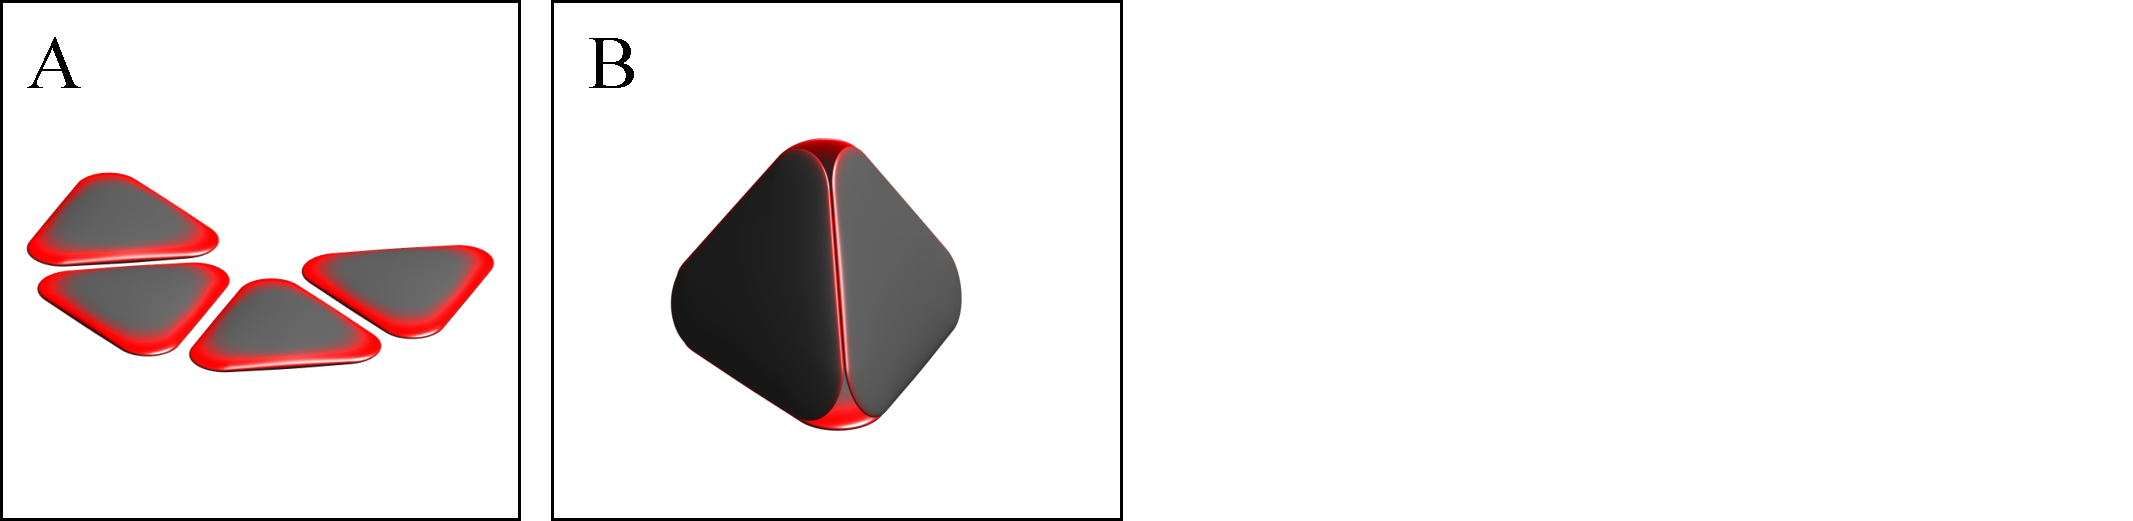
\includegraphics[width=3.0in]{figures/SA3_fig2.pdf}}
\vspace*{5pt}
\caption{{\footnotesize Illustration of self-assembly of hydrophobically labeled faces.
The thick triangles have a rim-hydrophobic label on one side, and are hydrophilic on the other side.
These shapes would potentially aggregate into a tetrahedral container. }}
\label{fig:illustration}
\end{wrapfigure}
The HAP theory is ideally suited to the problem of creating microstructures through capillary action. Specifically, the modeling application considers the assembly of polyhedra from smaller subunits. Our developments, which include viscous interactions, thermal fluctuation, and a long range description of capillarity, will pave the way for dynamical understanding to organizational principles in viral capsid formation, for instance \cite{CASPAR1962,Prasad2012}. 

In order to illustrate the novelty of our approach, it is helpful to first describe how current experimental and mathematical techniques deal with polyhedral assembly. Capillary origami uses lithography to etch faces out of a thin, elastic sheet \cite{Pandey2011,Reynolds2019}. The collection of faces form a so-called net, and this net self-folds into a three-dimensional polyhedron (Figure~\ref{fig:illustration}). The motivation is to create micro containers to mimc protein folding \cite{Reynolds2019}. Prediction of geometric structure from its subunits is non-trivial. That is because the final morphology depends on the net structure, physical interactions, and the surrounding media, and researchers have formulated optimality criteria for these nets \cite{Araujo2018,Pandey2011}. 

The experimental shapes are hundreds of microns in diameter. Thus, as a key distinction with HAP approach, the driving force for folding in capillary origami and related processes comes from surface energy of the hinges (e.g. soldered hinges that supply a surface tension once the system is heated). Mathematicians have numerically and analytically described the behavior of these surface tension driven hinges \cite{Bico2018,Peraud2014,Brubaker2016}, making it possible to simulate the mechanical problem, in principle, using slender body theory for plates. 

To study this problem using HAP theory, we form a collection of thin, prism-like particles in Figure \ref{fig:illustration}. 
Each of these particles serves as a face in the final morphology. The edges of the prisms are labeled hydrophobic according to the boundary condition in the screened Laplace equation boundary value problem. This way, the edges coalesce, forming the desired structures. Furthermore, 
by manipulating the boundary condition in HAP, it is possible to have faces attach and detach with precision, and form a net or other structures if so desired. Our HAP theory therefore generalizes submillimeter theoretical and experimental work to the micron and nanometer sizes. 

%There is also the possibility to explore new classes of mathematical materials, like wrinkling in polystyrene sheets \cite{Paulsen2016}, that include the interaction between an elastic material, the viscous solvent, and long range hydrophobic (capillary) interactions. In the case of rigid particles and subunits, the rigid body motions come from the so-called mobility boundary value problem for the Stokes equation. Here, the hydrophobic stress balances with the viscous stress coming from the rigid body motion of the particles in the surrounding solvent. If the particles are deformable, like a protein \cite{Elms2012} or as in the capillary induced bending of rods \cite{Schulman2017}, then we can formulate an elastic energy for deformation. These elastic energies account for surface bending or even permanent charge. To deploy this approach, it is a matter of solving the bodies' momentum balance equations coupled to the fluid through the viscous, elastic, and hydrophobic stress balance. 

\begin{figure}
\begin{center}
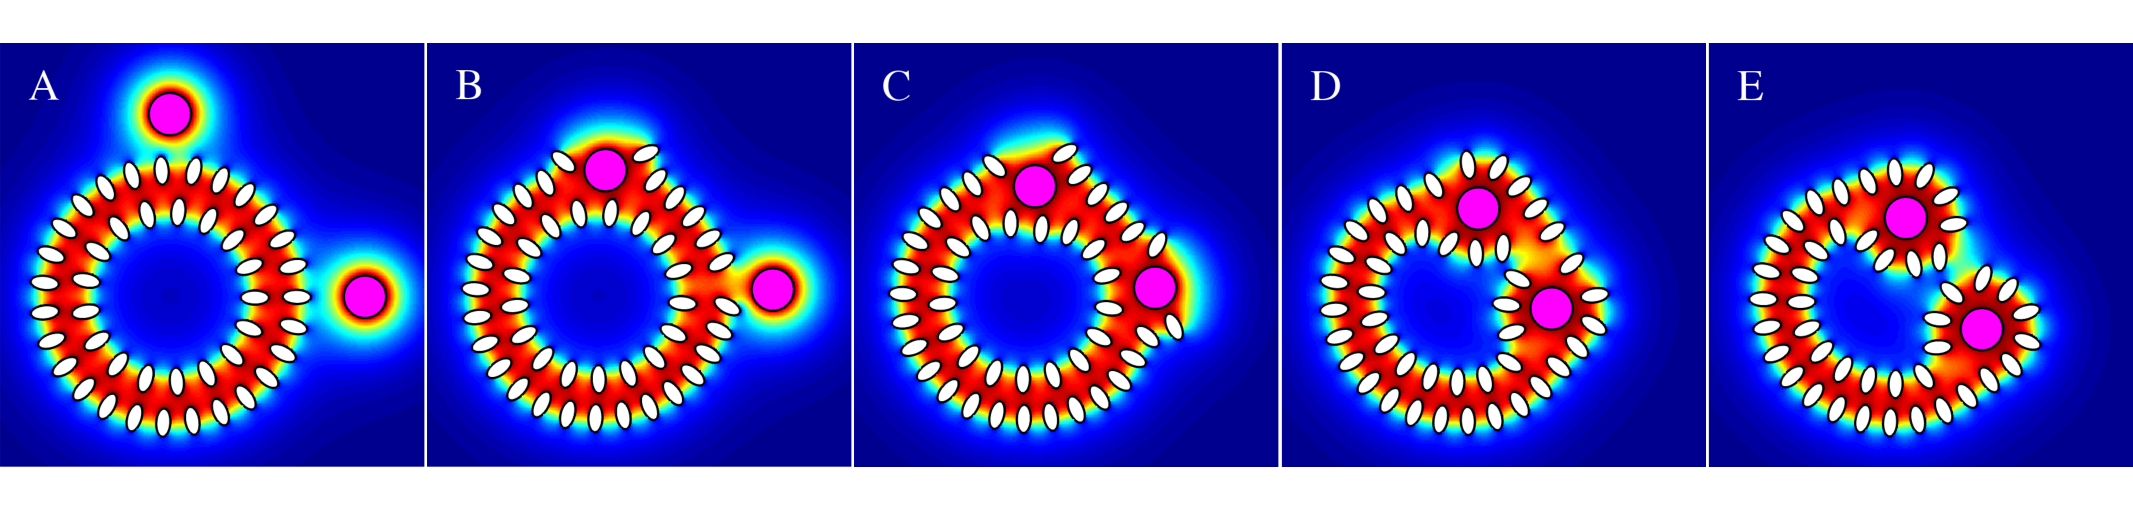
\includegraphics[width=\textwidth]{figures/SA3_fig1.pdf}
\end{center}
\caption{(A)--(D) shows the spontaneous insertion of two hydrophobic particles into a vesicle bilayer. 
The driving force is long-range interaction between the hydrophobic, magenta particles and
the bilayer core.  The particle entrainment cause the vesicle to break apart, analogously to surfactant
induced lysis.}
\end{figure}
Finally, further applications of our modeling approach include colloidal interaction on interfaces. Here, the experimental setups use Janus particles to model, for example, membrane bound proteins \cite{Kumar2013,Lehle2008,Zhang2017}. The idea of an amphiphilic Janus particle was introduced by P. G. de Gennes in 1991 \cite{Zhang2017}. The Investigators have significant experience as Janus particles figure heavily into our particle based description of bilayers, and can adjust our modeling approach to account for proteins. This is done by consider mixtures, consisting of many (hundreds to thousands) long, elongated amphiphilic particles for the lipid phase. Larger particles with hydrophobic patches or stripes model the proteins \cite{Jurasek2017}.

The distinction between macroscopic capillarity and microscopic hydrophobic force are relevant here as well.  Prior models use surface energies to account for interaction between particles in an interface \cite{Dasgupta2017}. 
However, this may be missing important physics, and here our modeling approach has the advantage in that protein insertion, for instance, is a self-consistent consequence of the formulation, versus an assumption imposed by boundary conditions.  
The simulations will enable us address important biological questions on how a collection of 
interface bound colloids interact \cite{Yao2013,Salib2013}, 
and how configurations dictate 
macroscopic surface properties and sense background curvature \cite{Cavallaro2011,Liu2018,Sharifi-Mood2015}. 


\newpage

\subsection{Specific Aim 3: Efficient high-order numerical methods for
large-scale simulations}
\label{subsec:specific_aim_3}
% ----------------------------------------------------------------------
The HAP model requires solving the exterior Dirichlet problem of the
screened Laplace equation and the mobility problem of the Stokes flow at
each time step in the complex domains such as Figure~\ref{fig:domain}.
If discretizing these equations with stencil-based numerical methods,
the computational domain must be truncated, the volume must be
discretized, and artificial boundary conditions must be imposed. The
artificial boundary conditions introduces additional error, and
discretizing the volume results in an excessively large linear system.
Moreover, it is difficult to obtain high-order discretizations when the
boundary surfaces are irregular. Since we are solving
constant-coefficient elliptic PDEs, we represent the solution of the PDE
of interest as a layer potential 
\begin{align}
  \label{eq:LP}
  u(x) = \int_{\partial\Omega} K(x,y) \sigma(y) ds_y,
\end{align}
where $\sigma$ is an unknown density function, and $K(x,y)$ is formed
with derivatives of the fundamental solution of the underlying PDE. By
matching the boundary condition at $x_0 \in \partial\Omega$ with the
limit of equation~\eqref{eq:LP} as $x\rightarrow x_0 \in
\partial\Omega$, a BIE for the density function is formed.
Numerical methods to solve BIE has several advantages over their
PDE-based counterpart: by construction, the layer
potential~\eqref{eq:LP} satisfies far-field conditions; only
$\partial\Omega$ needs to be discretized; carefully chosen kernels
$K(x,y)$ result in a well-conditioned linear system that requires a
mesh-independent number of GMRES iterations to solve; and high-order or
spectral accuracy is attainable by using appropriate quadrature methods.
In our previous work~\cite{Fu2018_SIAM} we demonstrate that BIEs are a
powerful tool to simulate two-dimensional suspensions of amphiphilic
particles. In addition to improving two-dimensional simulations, we will
extend the results to three dimensions using a standard
three-dimensional BIE of the screened Laplace equation~\cite{ying_2006}
and a well-conditioned BIE of the mobility problem~\cite{manasthesis}.

The most significant challenges of a BIE formulation include solving
dense linear systems, developing preconditioning strategies, and
developing quadrature methods for integrands that are nearly singular.
These challenges are described in section~\ref{subsec:NumericalIssues}.
Then, in section~\ref{subsec:timeStepping}, time stepping strategies are
described, and stable BIE formulations for fluctuating hydrodynamics are
in section~\ref{subsec:fluctuating}.


% ----------------------------------------------------------------------
\subsubsection{Numerical issues}
\label{subsec:NumericalIssues}

Discretizations of carefully chosen BIEs can be solved with a
mesh-independent number of GMRES
iterations~\cite{cam-ips-kel-mey-xue1996}. Therefore, the required CPU
time is proportional to the cost of a matrix-vector multiplication that
can be done in optimal or near-optimal time with the fast multiple
method (FMM)~\cite{fmm5} and its extensions~\cite{fmm1, fmm2, fmm3,
fmm4, fmm6, fmm7, fmm8}. PI Quaife is experienced with applying FMMs for
both the Stokes equation~\cite{qua-bir2014, bys-sha-qua2020} and the
screened Laplace equation~\cite{kro-qua2011, qua2011}. Alternatively,
fast direct solvers can be used to avoid any iteration~\cite{fds1, fds2,
fds3, fds4, fds5, fds6, fds7, fds8, ho2016cpam2, ho2016cpam1,
minden2016, minden2017siammms}, but direct solvers often require a large
amount of initial overhead, and this makes them less useful for problems
with moving geometries.  Alternatively, techniques in fast direct
solvers can be used to develop efficient preconditioning strategies. PI
Quaife used the inverse Fast Multipole Method
(IFMM)~\cite{cou-pou-dar2017, qua-cou-dar2018} to precondition Stokes
equations in a porous media, and a suite of preconditioners ranging from
block-diagonal to the IFMM will be considered.  

Nearly touching bodies is ubiquitous in self-assembly of amphiphilic
particles, and such near-contact results in nearly-singular integrands
in both two and three dimensions. Quadrature methods to address such
integrands has received a lot of attention in two and three
dimensions~\cite{alpert, kapur, sidi, duffy, bruno1, bruno2, davis_1984,
graglia_2008, hackbusch_sauter_1994, jarvenpaa_2003, khayat_2005,
schwab_1992, ying_2006, beale1, beale2, goodman_1990, haroldson_1998,
lowengrub_1993, schwab_1992, ggq1, ggq2, ggq3, helsing_2008a,
helsing_integral_2009, helsing_tutorial_2012, klockner2013jcp, qbx2,
wala2019jcp, af2018sisc, siegel2018jcp, rachh2017jcp, ding2019arxiv,
bar2014}. For two-dimensional problems, the trapezoid rule is the
workhorse for BIEs since it achieves spectral accuracy when integrands
are not nearly-singular~\cite{tre-wei2014}. To address nearly-singular
integrands of two dimensional BIEs, we will use a {\em barycentric
quadrature rule} that only requires a slight modification of the
trapezoid rule~\cite{ioa-pap-per1991}. In its current form, this method
requires the layer potential satisfy Laplace or Stokes
equations~\cite{bar-wu-vee2015, chi-moo-qua2020}. The PIs will extend
this quadrature rule so that it can be applied to the screened Laplace
equation. This will be done by recognizing that the fundamental solution
of the screened Laplace equation can be decomposed as $K(x,y) = K_1(x,y)
+ K_2(x,y)$, where $K_1(x,y) = -\log\|x - y\|$ and $K_2(x,y) = K(x,y) +
\log\|x - y\|$. Using this decomposition, the layer potential involving
$K_1(x,y)$ can be accurately computed with the barycentric quadrature
rule~\cite{ioa-pap-per1991}, and the layer potential $K_2(x,y)$ can be
accurately computed with the trapezoid rule since the kernel is bounded
for all $x$ and $y$.
\todo[inline]{Image here}

% ----------------------------------------------------------------------
\subsubsection{Avoiding contact with adaptive time stepping and
repulsion}
\label{subsec:timeStepping}
\todo[inline]{Put contact in here as well}
\todo[inline]{Adaptive high-order time stepping}

Even with accurate quadrature and time stepping methods, rigid body
simulations can still result in unphysical contact. We proposed to use
two techniques to avoid unphysical contact: high-order adaptive time
stepping and a repulsion force. PI Quaife developed a high-order
adaptive time stepping method for hydrodynamic
suspensions~\cite{qua-bir2016} and he has used it with colleagues to
investigate mixing and adhesion in suspensions~\cite{qua-vee-you2019,
kab-qua-bir2017}.



In our previous work a
Leonard-Jones potential is used to keep the particles from
overlapping~\cite{Fu2018_SIAM}. Such steep steric interaction at short
ranges introduces great numerical stiffness that limit the time step
size. 
\cite{bys-sha-qua2020}


\textcolor{red}{
Another outstanding numerical issue pertaining to simulating the
self-assembly of amphiphilic particles (such as lipid macromolecles) in
a viscous solvent is the collision between amphiphilic particles. The
hydrophobic attraction potential drives the amphiphilic particles to
move towards each other so to minimize exposure to the solvent. Under
such attraction force the fluid is being squeezed out as particles move
toward each other, and the amphiphilic particles can come into physical
contact in finite time. Such particle collisions in a dense rigid body
suspension is a great challenge and can be a bottleneck in large-scale
simulations. In our previous work a Leonard-Jones potential is used to
keep the particles from overlapping~\cite{Fu2018_SIAM}. Such steep
steric interaction at short ranges introduces great numerical stiffness
that limit the time step size. 
}

\textcolor{red}{
Yan {\it et al.} proposed a collision-resolution algorithm within the
framework of boundary integral methods to resolve the non-smooth
many-body dynamics due to collisions by formulating the particle
collision process as a linear complementarity problem with geometric
`non-overlapping' constraint~\cite{Yan2019}. We propose to treat the
particle collisions based on Yan {\it et al.}'s work after the first two
goals (see above) are achieved. A potential complication in combining
the algorithms for particle collision into our QBX integral formulation
is the computational cost for the QBX to refine meshes on particles in
collision.
}

\textcolor{red}{
Once the collision-resolution algorithm is implemented, we will check
the computing performance first before we embark on incorporating
fluctuating hydrodynamics~\cite{Bao17,Bao18}, which might be important
even at the scales of the amphiphilic particle size in some cases. We
propose to extend the high-order time-integration scheme for a
stochastic differential equation~\cite{fu2015pre} to this system.
}


% ----------------------------------------------------------------------
\subsubsection{Fluctuating hydrodynamics}
\label{subsec:fluctuating}
Using DLP formulation for fluctuating hydrodynamics so that we have a
second-kind BIE



%The HAP model requires solving the exterior Dirichlet problem of the
%screened Laplace equation and the mobility problem of the Stokes flow
%at each time step. Standard numerical methods such as finite difference
%and finite element methods have to truncate the infinite domain to a
%finite computational domain by imposing certain artificial boundary
%conditions on the truncated domain and need the discretization of the
%whole volume of the truncated domain. The artificial boundary
%conditions are very often inexact, introducing another layer of
%approximation that lowers the accuracy of the solution. The
%discretization of the whole volume is very expensive for three
%dimensional problems, leading to excessively large number of unknowns
%in the linear system. Furthermore, it is rather difficult to obtain
%high-order discretization when the boundary surfaces are irregular.

%Potential theory and boundary integral equation (BIE) methods remove the
%aforementioned obstacles in a very elegant way. The starting point is
%that for constant-coefficient PDEs the fundamental solutions, i.e., the
%Green's functions, are readily available. This allows us to represent
%the solution via the so-called layer potentials that are the convolution
%integrals of a kernel and an unknown density only on the boundary. The
%kernel is a linear combination of the Green's function and its
%derivatives, which ensures that the representation satifies the
%underlying PDE and the condition at infinity automatically. And the
%boundary condition at the material interfaces together with the jump
%relation of the layer potential leads to a boundary integral equation
%for the unknown density.
 
%The BIE method removes the need of imposing artificial boundary
%conditions for exterior problems and reduces the dimension of the
%problem by one, leading to optimal number of unknowns in the solve
%phase. Very often, one is able to construct the so-called {\it second
%kind integral equation} (SKIE) formulation for these problems, where
%the operator is a sum of the identity operator and a compact operator.
%It is well-known that the condition number of the resulting linear
%system for SKIEs is {\it independent} of the mesh size $h$ or
%equivalently, the number of discretization points. This leads to a
%constant number of iterations when iterative solvers are applied to
%solve the resulting linear system. It further improves the accuracy of
%the solution as the relative error of solution will never increase as
%the number of total discretization points increases. On the other hand,
%the condition number of the linear system from finite difference and
%finite element methods generally increases as a power function of the
%total number of dicretization points, with the exact power depending on
%the underlying spatial dimension and the highest order of the
%differential operator in the PDE. This leads to an increase in the
%number of iterations (and hence the total computational cost) and an
%increase in the relative error of the solution as the number of
%dicretization points increases.

%The discretization of the integral operator often leads to a dense
%matrix, while finite difference/finite element methods result in sparse
%matrices, making matrix-vector product much cheaper to compute.
%However,since the invention of the original fast multipole method
%(FMM)\cite{fmm5}, there have been many fast
%algorithms~\cite{fmm1,fmm2,fmm3,fmm4,fmm6,fmm7,fmm8} that reduce the
%cost of matrix-vector product to linear ($O(N)$) or quasilinear
%complexity ($O(N \log^kN)$) for dense matrices resulting from the BIE
%discretization. Fast direct solvers have also been developed
%recently~\cite{fds1,fds2,fds3,fds4,fds5,fds6,fds7,fds8,ho2016cpam2,ho2016cpam1,minden2016,minden2017siammms}.
%The development of these fast algorithms have removed a huge hurdle for
%the use of boundary integral equations, making the BIE method the
%method of choice for constant-coefficient PDEs with linear boundary
%conditions.  For the exterior Dirichlet problem of the screened Laplace
%equation, the SKIE formulation in our previous work~\cite{Fu2018_SIAM}
%can be readily extened to the 3D case. For the mobility problem of the
%Stokes flow in three dimensions that takes the hydrodynamic effect into
%account, an SKIE formulation can be found in~\cite{manasthesis}.

%% ----------------------------------------------------------------------
%\subsubsection{High-order discretization of surface integrals in three
%dimensions}
%The practical application of integral equation methods requires the
%accurate evaluation of boundary integrals with singular, weakly singular
%or nearly singular kernels. There are many numerical quadrature schemes
%for dealing with line integrals in two
%dimensions~\cite{alpert,kapur,sidi,duffy,bruno1,bruno2,davis_1984,graglia_2008,hackbusch_sauter_1994,
%jarvenpaa_2003,khayat_2005,kress_boundary_1991,schwab_1992,
%ying_2006,beale1,beale2,goodman_1990, haroldson_1998,
%lowengrub_1993,schwab_1992,ggq1,ggq2,ggq3,helsing_2008a,helsing_integral_2009,helsing_tutorial_2012}
%and some of them are extremely efficient and can achieve arbitrary high
%order.
%
%The high-order quadrature rules for the evaluation of surface integrals
%in three dimensions, however, are much less developed than the line
%integrals in two dimensions. For example, there are no Gaussian
%quadratures for integraing polynomials on a flat triangle, even though
%efficient quadratures~\cite{xiao2010cma,vioreanu2014} have been
%developed recently for such purpose. For weakly singular or singular
%integrals,~\cite{bremer2012jcp,bremer2013jcp} constructed high-order
%quadratures for surface integrals on a general triangle,
%while~\cite{gimbutas2013sisc} presented a fast algorithm for integrating
%$1/r$-type singular integrals for surfaces that are homeomorphic to a
%sphere. We plan to study the so-called quadrature by expansion (QBX)
%scheme~\cite{klockner2013jcp,qbx2} for the evaluation of both singular
%and near-singular surface integrals encountered in the discretization of
%BIEs in three dimensions. Conceptually, the idea of the QBX to evaluate
%singular, hypersingular and near singular integrals on smooth surfaces
%is straightforward. That is, the surface is discretized into smooth
%triangles and smooth high-order quadratures are applied to evaluate the
%expansion coefficients on all source triangles with the QBX expansion
%center placed at a point off the surface. One may then form a suitable
%expansion (for example, a Taylor expansion) around that center and
%evaluate this expansion back at the target point on the surface (or
%close to the surface in the near singular case). Compared to the
%competing aforementioned quadrature schemes, the QBX quadrature is
%attractive because it offers a clear path for being extended to:
%\textbf{(1)} handle any singularity, including hypersingular operators,
%\textbf{(2)} be usable with any high-order surface discretization,
%\textbf{(3)} generate well-conditioned discrete operators to which
%iterative methods such as GMRES~\cite{gmres} can be applied in a
%black-box fashion, \textbf{(4)} integrate well with fast algorithms such
%as the FMM. 
%
%In practice, there are still many issues that need to be resolved. For
%example, there are now many variants of QBX including global and local
%QBX~\cite{klockner2013jcp,rachh2017jcp}, the target-specific
%QBX~\cite{siegel2018jcp}, kernel-independent QBX~\cite{abtin2018bit},
%and quadrature by two expansions~\cite{ding2019arxiv}. The coupling of
%the QBX and the FMM may also lead to certain instability issues which
%may require some changes in the fast multipole
%method~\cite{wala2018jcp}. Similar to other quadrature methods, there
%have been extensive study on the QBX methods in two dimensions, while
%its three dimension
%version~\cite{wala2019jcp,af2018sisc,siegel2018jcp,wala2019arxiv} has
%not been fully studied and the implementation is even more scarce. We
%plan to investigate the accuracy and the convergence order of the
%various QBX schemes mentioned above, its coupling with the FMM, parallel
%implementation issues for large-scale problems, and the application to
%our target problems.

%% ----------------------------------------------------------------------
%\subsubsection{A hybrid method for close-to-touching Janus particles}
%\textcolor{red}{
%The HAP model for membranes will inevitably lead to the case where some
%Janus particles will be very close to each other. Even though QBX can
%handle such case accurately, it may lead to excessively large number of
%unknowns in order to resolve the unknown densities at those
%close-to-touching points. In~\cite{gan2016sisc}, a hybrid scheme is
%developed to treat the close-to-touching spheres for the interface
%problem of the Laplace equation. The key idea is to combine the analytic
%image method and spectrally accurate method of moments, where the
%analytic image method will capture the most singular part of the unknown
%density at the close-to-touching points. With the aid of the FMM, the
%scheme achieves linear complexity with much less number of unknowns on
%the material interfaces. We plan to study the hybrid scheme to treat
%the close-to-touching case for both the screened Laplace equation and
%the mobility problem to further improve the efficiency of the numerical
%algorithm for the HAP model.
%}
%
%
%% ----------------------------------------------------------------------
%\subsubsection{Other numerical issues}
%Another outstanding numerical issue pertaining to simulating the
%self-assembly of amphiphilic particles (such as lipid macromolecles) in
%a viscous solvent is the collision between amphiphilic particles. The
%hydrophobic attraction potential drives the amphiphilic particles to
%move towards each other so to minimize exposure to the solvent. Under
%such attraction force the fluid is being squeezed out as particles move
%toward each other, and the amphiphilic particles can come into physical
%contact in finite time. Such particle collisions in a dense rigid body
%suspension is a great challenge and can be a bottleneck in large-scale
%simulations. In our previous work a Leonard-Jones potential is used to
%keep the particles from overlapping~\cite{Fu2018_SIAM}. Such steep
%steric interaction at short ranges introduces great numerical stiffness
%that limit the time step size. 
%
%Yan {\it et al.} proposed a collision-resolution algorithm within the
%framework of boundary integral methods to resolve the non-smooth
%many-body dynamics due to collisions by formulating the particle
%collision process as a linear complementarity problem with geometric
%`non-overlapping' constraint~\cite{Yan2019}. We propose to treat the
%particle collisions based on Yan {\it et al.}'s work after the first two
%goals (see above) are achieved. A potential complication in combining
%the algorithms for particle collision into our QBX integral formulation
%is the computational cost for the QBX to refine meshes on particles in
%collision.
%
%Once the collision-resolution algorithm is implemented, we will check
%the computing performance first before we embark on incorporating
%fluctuating hydrodynamics~\cite{Bao17,Bao18}, which might be important
%even at the scales of the amphiphilic particle size in some cases. We
%propose to extend the high-order time-integration scheme for a
%stochastic differential equation~\cite{fu2015pre} to this system.


\section{Broader Impacts of the Proposed Work}
\label{sec:BroaderImpacts}

The proposed mathematical analysis, modeling, and numerical algorithms
will transform our understanding of the collective dynamics of
amphiphilic particles such as (1) their self-assembly into micelles and
bilayers, (2) the material properties of such self-assembly, and (3) the
interaction between these building blocks. In addition to biophysical
applications, amphiphilic Janus particles have recent popularity in the
fabrication of smart materials. The proposed work will have a
transformative impact on precision design for specific mechanical
properties of materials made of amphiphilic nanoparticles. An important
component of this proposal is the interdisciplinary education and
training of both undergraduate students, graduate students, and
postdoctoral fellows. The combination of mathematical modeling,
analysis, and scientific computing in this project provides a compelling
example of the importance of mathematics in biophysics and engineering
applications. The concepts and methods described here go beyond the
context of amphiphilic particles and lipid molecules. They extend to
other problems featuring microscopic phase separation that leads to
formation of mesoscopic domains. This situation arises, for example, in
biological development in systems biology. The methods developed here
have the potential to impact those and other related areas in
biomedicine and biotechnology.

\subsection{Educational Impacts}
\label{subsec:Educational_plans}
The proposed research will have an immediate impact on undergraduate and
graduate education. At the undergraduate level, the project will include
and support undergraduate researchers from Fordham University. The
supported summer researchers will gain valuable first-hand
interdisciplinary experience in mathematical modeling and computation.
We will incorporate research into teaching, especially in differential
equation and programming courses. PI YNY will work on simple modeling of
self-assembly problems with both undergraduate and high school students
from Newark Science Park High School. PI YNY has a track record of
working with local high school students for their research projects
before they apply for colleges. PI BQ will work with undergraduate and
high school students through the Undergraduate Research Opportunity
Program and Young Scholar's Program as he has done in the past.

Over the past eight years, PI RR has included many undergraduates in the
execution of research initiatives and coauthoring publications. He has a
track record for supporting underrepresented groups, being called on by
the Collegiate Science and Technology Entry Program (CSTEP) to make
opportunities for promising students, for example. He has mentored two
Clare Boothe Luce Scholars, one a U.S.~Marine Corp veteran, and a high
school student in the NYU GSTEM program. 

The PIs will capitalize on the synergy between both FSU's doctoral
program in Scientific Computing, NJIT's doctoral program in Mathematical
Sciences, and Fordham's undergraduate focus in the Department of
Mathematics. Promising, young undergraduate scientists from the Bronx
community will find a natural pipeline into graduate studies by working
directly or indirectly on this project. At the graduate-level, PI YNY
expects to train and support a PhD student for two more years. PI BQ
will advise a postdoctoral fellow for two years. The PIs will foster
vertical integration between the senior personnel, their collaborators,
postdocs, doctoral, and Bachelor students, enhancing the learning
environment.

%The PIs expect
%to involve undergraduate students in this project through
%their continuing and active involvement in undergraduate advising and research mentoring:
%YNY has mentored undergraduate students as a co-Investigator in CSUMS: Research and Education
%in Computational Mathematics for undergraduates in the Mathematical 
%Sciences at NJIT (funded by NSF) and the lecturer for Capstone Applied
%Mathematics Lab at NJIT (also funded by NSF).
%YNY has track records in involving undergraduate students in research
%that emphasizes both numerical computations and desktop experiments.
%
%such as MATH 340: Advanced Numerical Methods.
%Simple MATLAB codes have been used as teaching tools to show students how to use MATLAB
%to simulate the slender-body equations for an elastic filament in Stokes flow.
%
%In the past year YNY has been mentoring Ufuomaefe Ogbe, a high school student
%from Newark. Ufuomaefe is an African American who 
%worked with PI on a simplified model for vesicles in flow. Based
%on what he learned about modeling and programming, 
%he has applied to the Applied Mathematics/Computer Science programs at both NJIT
%and Rutgers/Newark.

\section{Intellectual Merit}
A central theme of the project is the mathematical development and
analysis of the physical model for interaction between many amphiphilic
particles. The model formulates the interaction potential through a
screened Laplace equation boundary value problem possessing the physical
properties like non-additivity and decay of realistic hydrophobic
attraction. Colloidal systems collectively self-assemble into bilayer
morphologies, and we analyze the elastic properties of these amphiphilic
particle ensembles. This allows us to interpret the Helfrich free energy
in terms of hydrophobic interactions and specific molecular
characteristics. We extend the capabilities of the boundary integral
equation and time stepping methods to stably perform large particle
number simulations in three dimensions. Results from these computations
will be used to compare collective amphiphilic against experiments and
to study the optimal design of three-dimensional functional materials. 




\newpage
\setcounter{page}{1}
\addcontentsline{toc}{section}{Bibliography}
\bibliographystyle{abbrvnat}
%
\bibliography{bibs/refs}
%\bibliography{bibs/references,bibs/analysis,bibs/computing,bibs/elastic,bibs/fmm,bibs/functionalmaterials,bibs/hydrophobic,bibs/jiang,bibs/journalnames,bibs/qbx,bibs/selfassembly,bibs/morerefs}
%\bibliography{bibs/analysis,
%	bibs/computing,
%	bibs/elastic,
%	bibs/fmm,
%	bibs/functionalmaterials,
%	bibs/hydrophobic,
%	bibs/jiang,
%	bibs/journalnames,
%	bibs/qbx,
%	bibs/references,
%	bibs/selfassembly}

%\input{references}



\end{document}
